\documentclass[t,14pt,aspectratio=169]{beamer}
\usepackage{ep-dark}   % JHU/WSE style for use on Lightboard
\usepackage{graphicx}  % for inclusion of graphics
\usepackage{amsmath}   % good for additional math
\usepackage{amsthm}    % theorems, definitions, etc

%\usetheme{CambridgeUS}

%% Oh yes. TIKZ pictures / graphs
%% -------------------------------------
\usepackage{tikz}
\usepackage{pgfplots}
\usepackage{tikz-3dplot}
\usepackage{tkz-euclide}
\usepackage[siunitx]{circuitikz}
\usetikzlibrary{calc,fadings,decorations.pathreplacing,shadings,intersections,backgrounds,angles,quotes,patterns}

%% This is when making tikz plots
%% -------------------------------------
\pgfplotsset{rdstyle/.style={%
        width=8cm,
        ylabel={y},
        xlabel={x},
        xmin=-2,xmax=3,
        xtick={-2,-1,...,3}}}
%% -------------------------------------

%% Axis rotator for arrows rotating around vector
%% -------------------------------------
\newcommand{\AxisRotator}[1][rotate=0]{%
    \tikz [x=0.25cm,y=0.60cm,line width=.2ex,-stealth,#1] \draw (0,0) arc (-150:150:1 and 1);%
}
%% -------------------------------------

\usepackage{asymptote}

%% Animations
%% -------------------------------------
\usepackage{animate}

%% This is the UT logo in the top right.
%% -------------------------------------
\logo {
\begin{tikzpicture}[overlay,remember picture]
\coordinate (A) at (-4.3,8.0);
\node[left=0.2cm] at (current page.27){
    
\includegraphics[width=3cm]{Figures/General/UT_WBMW_Rot_RGB_01.png}
    %
\includegraphics[width=3cm]{Figures/General/UT_WBMW_Weiss_1C_tr.png}
};
\node[text=Karminrot] at (A) {\tiny Introduction to Geophysics};
\end{tikzpicture}
}
%% -------------------------------------

%% -------------------------------------
%% Customized Environments

%%Empty column left, 1/3 filled right
%%Arguments is frametitle
\newenvironment{PointThree}[1]
{  \frametitle{#1}
  \begin{columns}[c, onlytextwidth]%EVEN SPECIFYING THE c OPTION
    \begin{column}{.6\textwidth}%
        \setlength{\partopsep}{0pt}%AND EVEN REMOVING EXTRA itemize SPACE
        % Keep this empty
    \end{column}%
    \begin{column}{.35\textwidth}
}
{
    \end{column}%
  \end{columns}
}
\newenvironment{PointSix}[1]
{  \frametitle{#1}
  \begin{columns}[c, onlytextwidth]%EVEN SPECIFYING THE c OPTION
    \begin{column}{.35\textwidth}%
        \setlength{\partopsep}{0pt}%AND EVEN REMOVING EXTRA itemize SPACE
        % Keep this empty
    \end{column}%
    \begin{column}{.6\textwidth}
}
{
    \end{column}%
  \end{columns}
}

%Input frame title and content left.
\newenvironment{ThreeCols}[2]
{
  \frametitle{#1}
  \begin{columns}[c, onlytextwidth]
    \begin{column}{.32\textwidth}%
        \setlength{\partopsep}{0pt}%AND EVEN REMOVING EXTRA itemize SPACE
        #2
    \end{column}%
    \begin{column}{.32\textwidth}
      %empty
    \end{column}%
    \begin{column}{.32\textwidth}

}
{
    \end{column}%
  \end{columns}
}
%% -------------------------------------




\title{Introduction to Geophysics}
\author{R. Drews}
\date{\today}


\begin{document}

% These commands create the first slide
% \coursename specifies the name of the course. No need to include the
% course number especially since they change from time to time
%
% \modulename is the name of this particular lesson

\coursename{Introduction to Geophysics}
\modulename{Resistivity Methods}
\titleframe

%
\begin{frame}
    % \small
    % \begin{PointSix}{How do we teach? }
    %     \begin{itemize}
    %         \item Video Lectures or Plenum (Tuesdays)
    %         \item Exercises \& 1-1-Interaction (Thursdays)
    %         \item Applied Exercises (Magnetics, Electrics, Seismics)
    %     \end{itemize}
    % \end{PointSix}
\end{frame}

\begin{frame}
  \begin{PointSix}{Introduction}
    \small
    \alert{Introduction to Geophysics}
    \begin{itemize}
      \item Who?
      \item What?
      \item How?
    \end{itemize}
  \end{PointSix}
  \end{frame}

\begin{frame}
    \begin{PointSix}{Who's teaching?}
        \small
        \begin{itemize}
            \item R. Drews (Prof. Geophysics at UT)
            \item P. Dietrich (Prof. Env./Eng.- Geophysics at UFZ, Leipzig)
            \item R. Ershadi (PhD Geophysics)
            \item A. Vinson (TA, MSc Geosciences)
            \item L. Naumann (TA, BSc Geosciences)
          \end{itemize}
    \end{PointSix}
\end{frame}

\begin{frame}
    \begin{PointSix}{Who's teaching?}
        \alert{Introduction to Geophysics - R. Drews}
        \small Prof. for Geophysics since 2022
      \end{PointSix}
\end{frame}

\begin{frame}
    \begin{PointSix}{Who's teaching?}
        \alert{Introduction to Geophysics - R. Drews}
        \small Prof. for Geophysics since 2022
        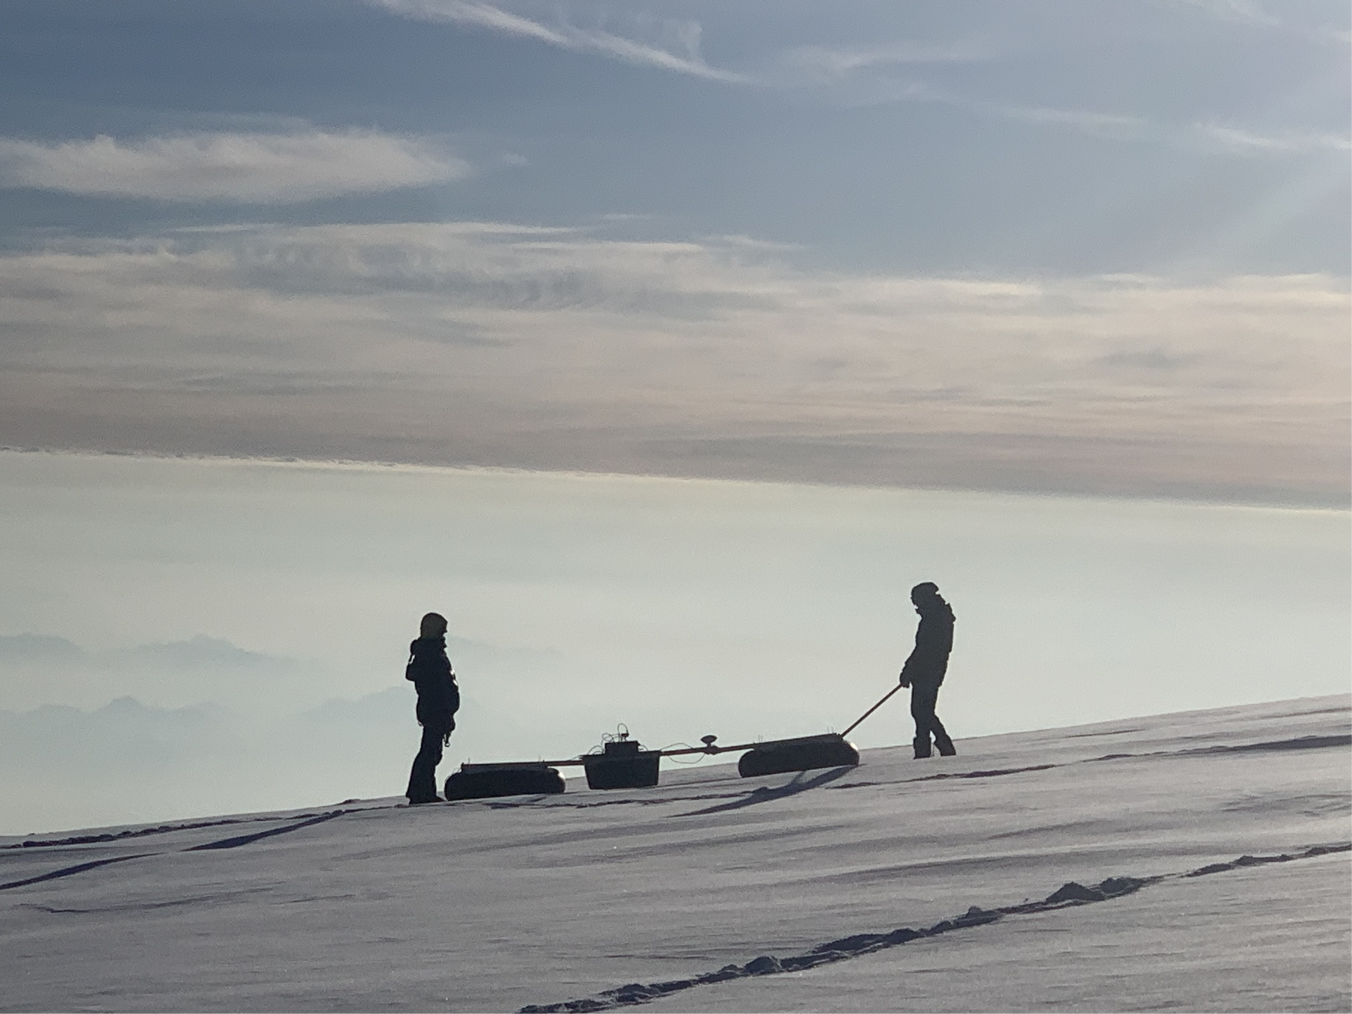
\includegraphics[width=0.99\textwidth]{Figures/General/FieldPhotos/GPRColle.png}
      \end{PointSix}
\end{frame}

\begin{frame}
    \begin{PointSix}{Who's teaching?}
        \alert{Introduction to Geophysics - R. Drews}
        \small Prof. for Geophysics since 2022
        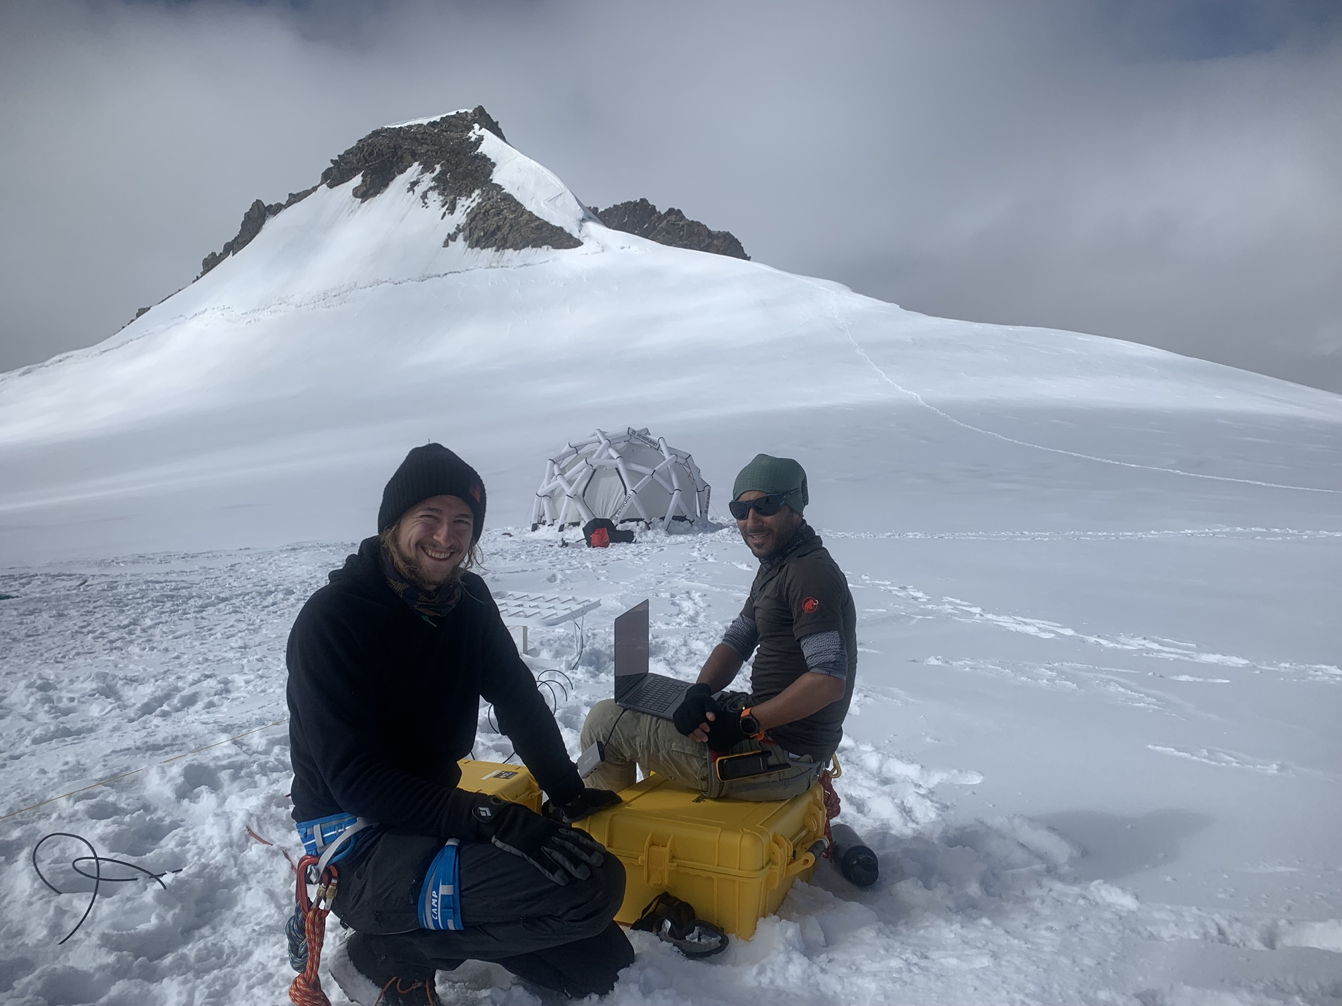
\includegraphics[width=0.99\textwidth]{Figures/General/FieldPhotos/GPRColle2.png}
      \end{PointSix}
\end{frame}

\begin{frame}
    \begin{PointSix}{Who's teaching?}
        \alert{Introduction to Geophysics - R. Drews}
        \small Prof. for Geophysics since 2022
        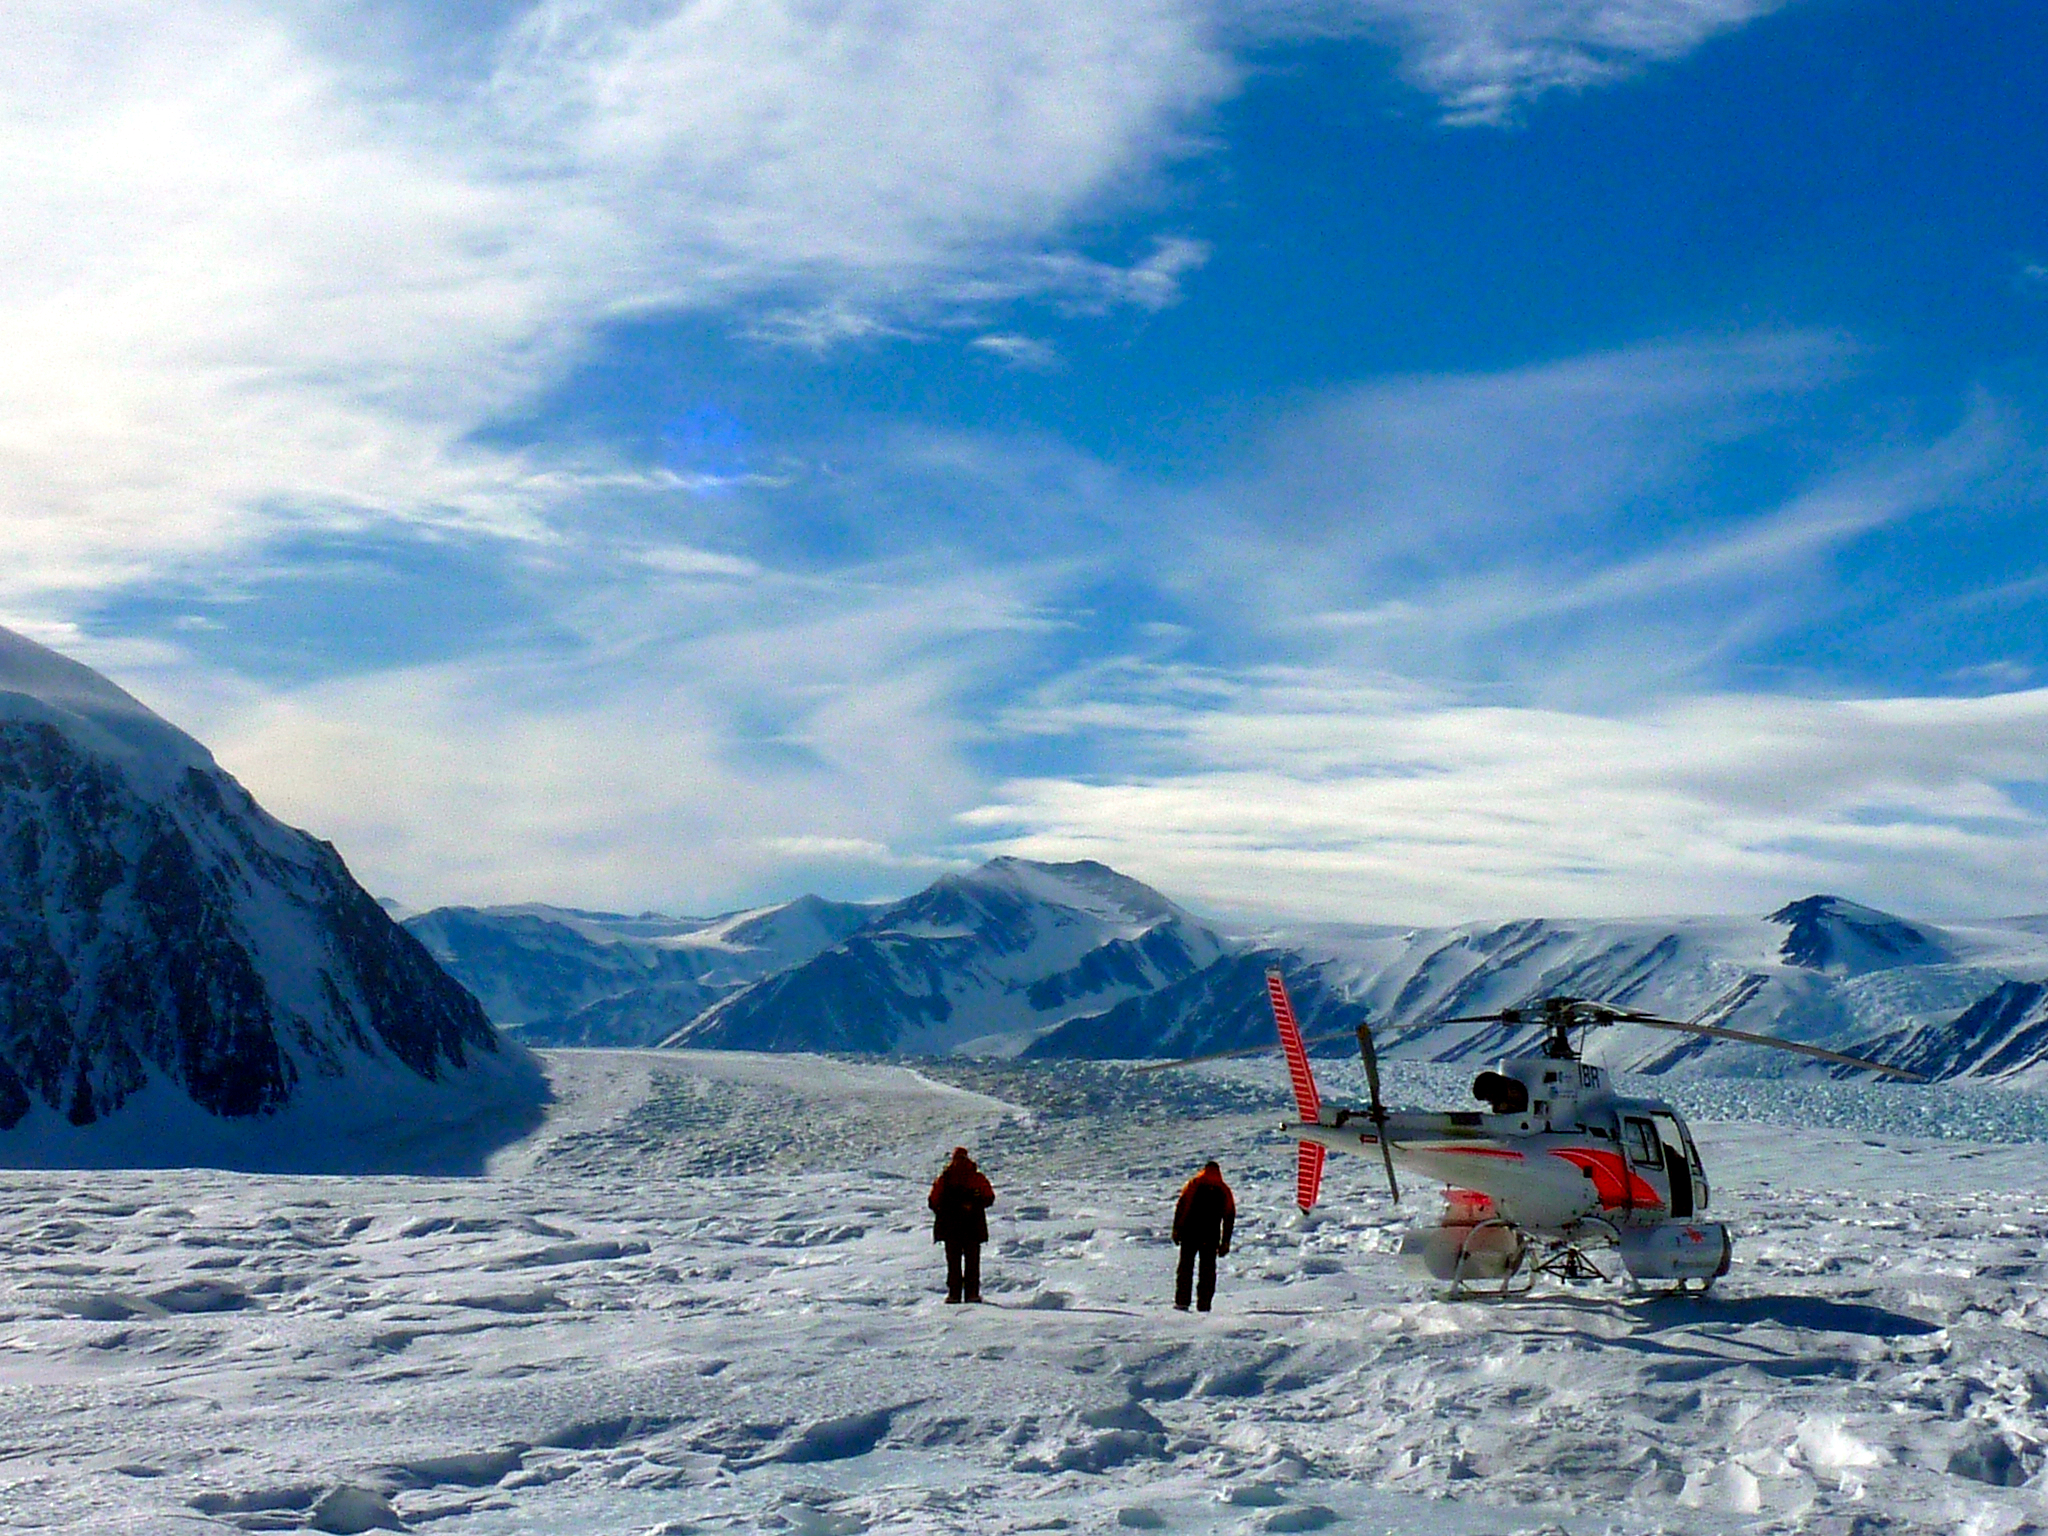
\includegraphics[width=0.99\textwidth]{Figures/General/FieldPhotos/PriestleyHelicopter.JPG}
      \end{PointSix}
\end{frame}

\begin{frame}
    \begin{PointSix}{Who's teaching?}
        \alert{Introduction to Geophysics - R. Drews}
        \small Prof. for Geophysics since 2022
        \includegraphics[width=0.99\textwidth]{Figures/General/FieldPhotos/GPRI.jpg}
      \end{PointSix}
\end{frame}

\begin{frame}
    \begin{PointSix}{Who's teaching?}
        \alert{Introduction to Geophysics - R. Drews}
        \small Prof. for Geophysics since 2022
        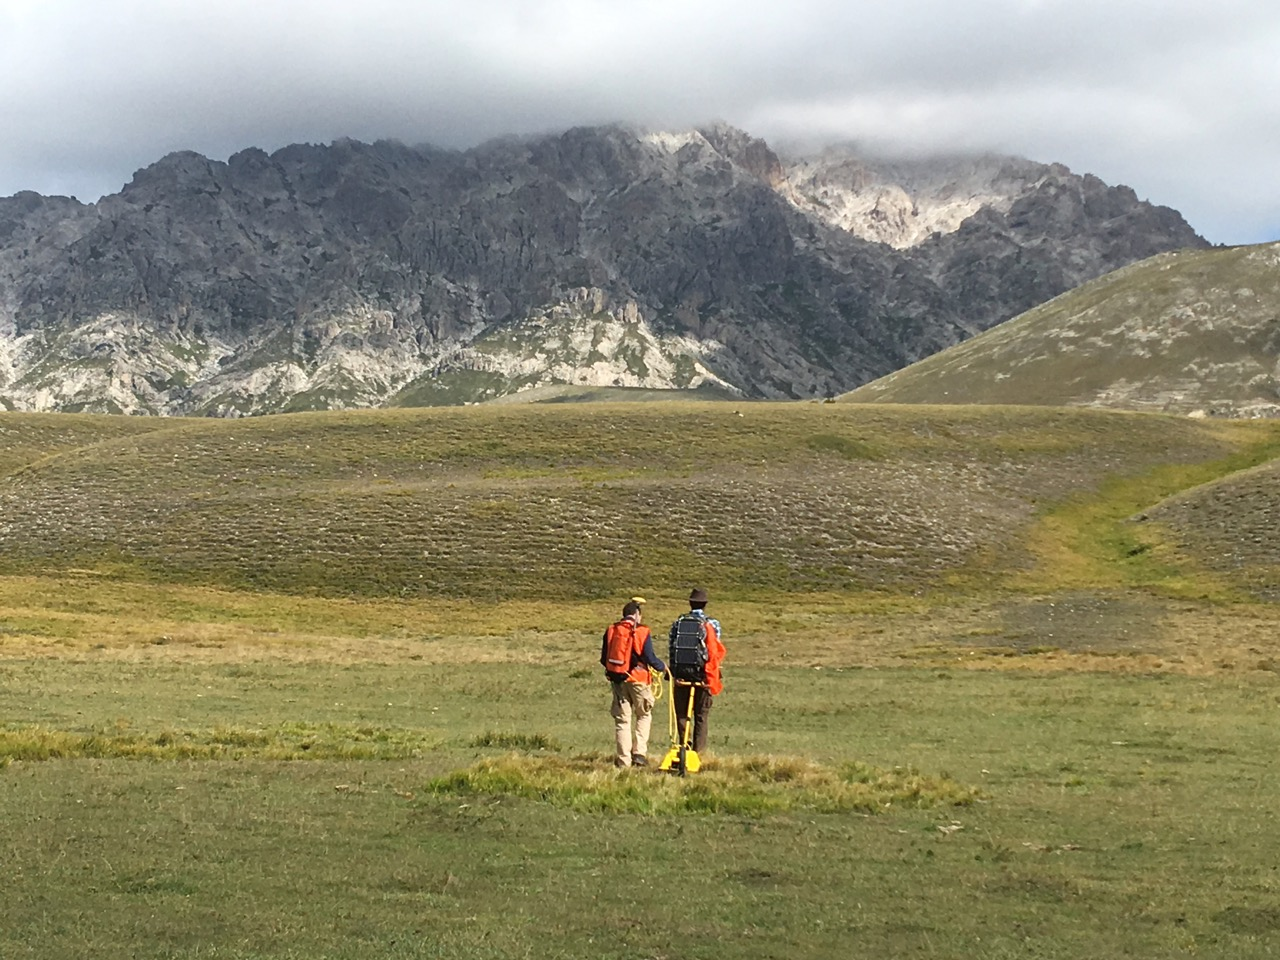
\includegraphics[width=0.99\textwidth]{Figures/General/FieldPhotos/ApenninsGPR.jpg}
      \end{PointSix}
\end{frame}


\begin{frame}
    \begin{PointSix}{What are we teaching?}
        \small
        \alert{Geophysics} is a branch of earth science dealing with the physical processes and phenomena occurring especially in the earth and in its vicinity.\\
        \vspace{0.25cm}
        \tiny [Merriam-Webster]\\
        \small
        \vspace{2.25cm}
        \alert{Applied Geophysics} is a branch of Geophysics dealing with different observational methods imaging the sub-surface.\\
        \vspace{0.25cm}
        \tiny [The lecture focus will be here.]
    \end{PointSix}
\end{frame}

\begin{frame}
    \begin{PointSix}{What are we teaching?}
        \small
        \alert{Applied Geophysics} contains, e.g, gravity, magnetics, electrics, electrical induction, electromagnetics (radar), seismics.\\
        \vspace{0.25cm}
        \tiny [Focus on physical principals rather than aquisition specifics.]
    \end{PointSix}
\end{frame}

\begin{frame}
    \begin{PointSix}{Example: Seismics}
        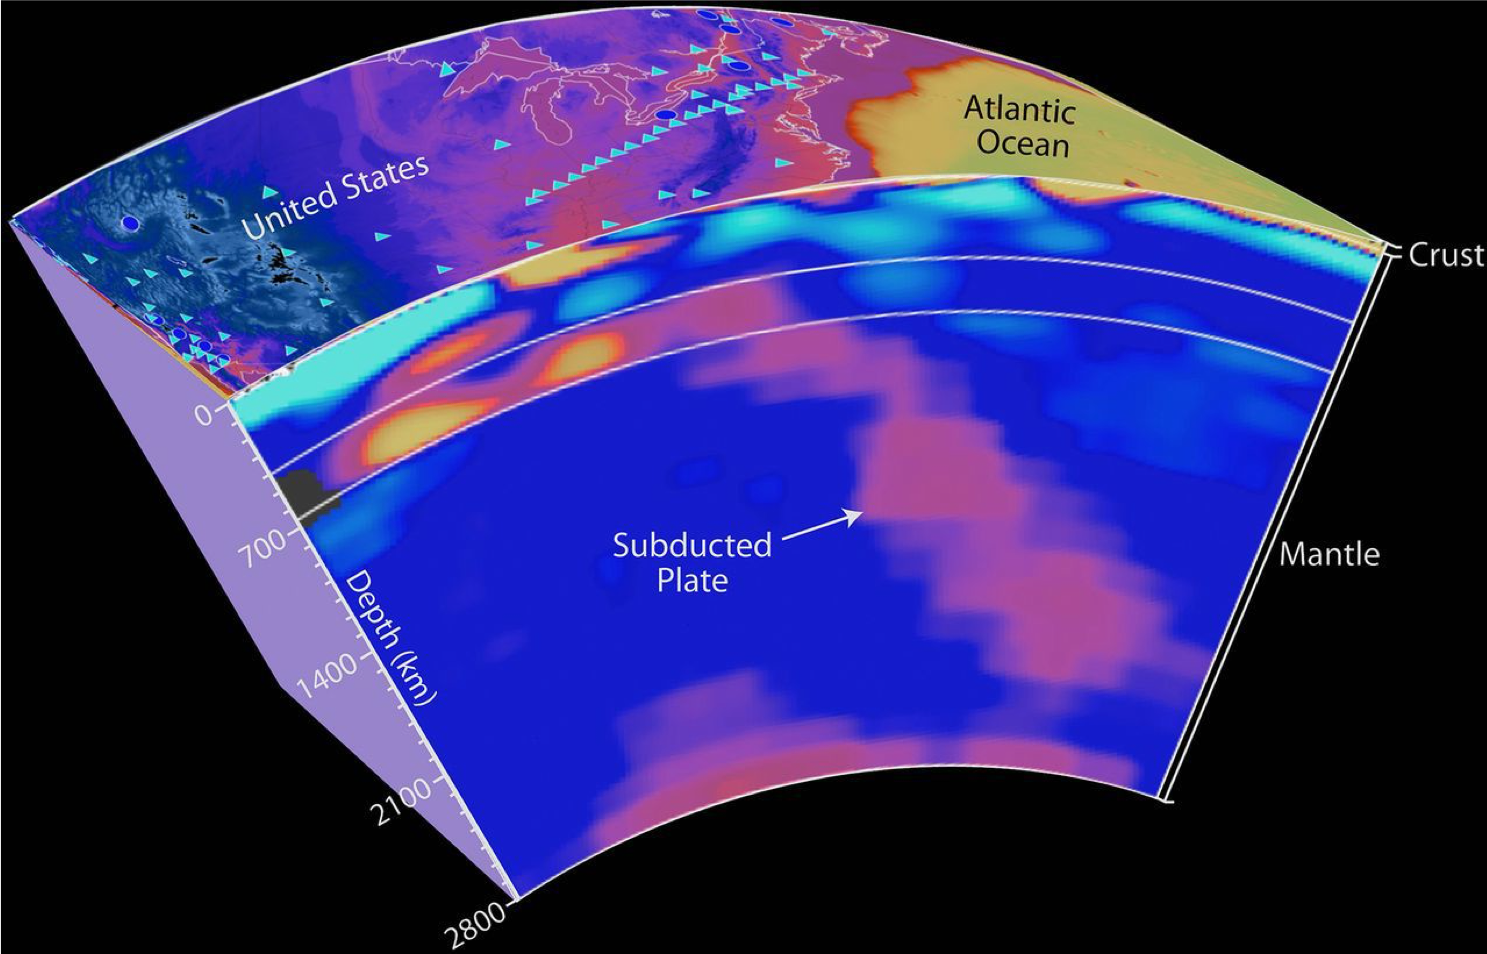
\includegraphics[width=0.99\textwidth]{Figures/General/GeophysExamples/Seismics_SvdLEE_Evanston_IL.png}
        \tiny[S. van der Lee, Northwestern University, Evanston, IL]
        %Data gathered by a network of seismic instruments (red) have enabled researchers to discern a region of relatively cold, stiff rock (shades of green and blue) beneath eastern North America. This is likely to be the remnants of an ancient tectonic plate. Image credit: Suzan van der Lee (Northwestern University, Evanston, IL).

    \end{PointSix}
\end{frame}

\begin{frame}
    \begin{PointSix}{Example: Magnetics}
        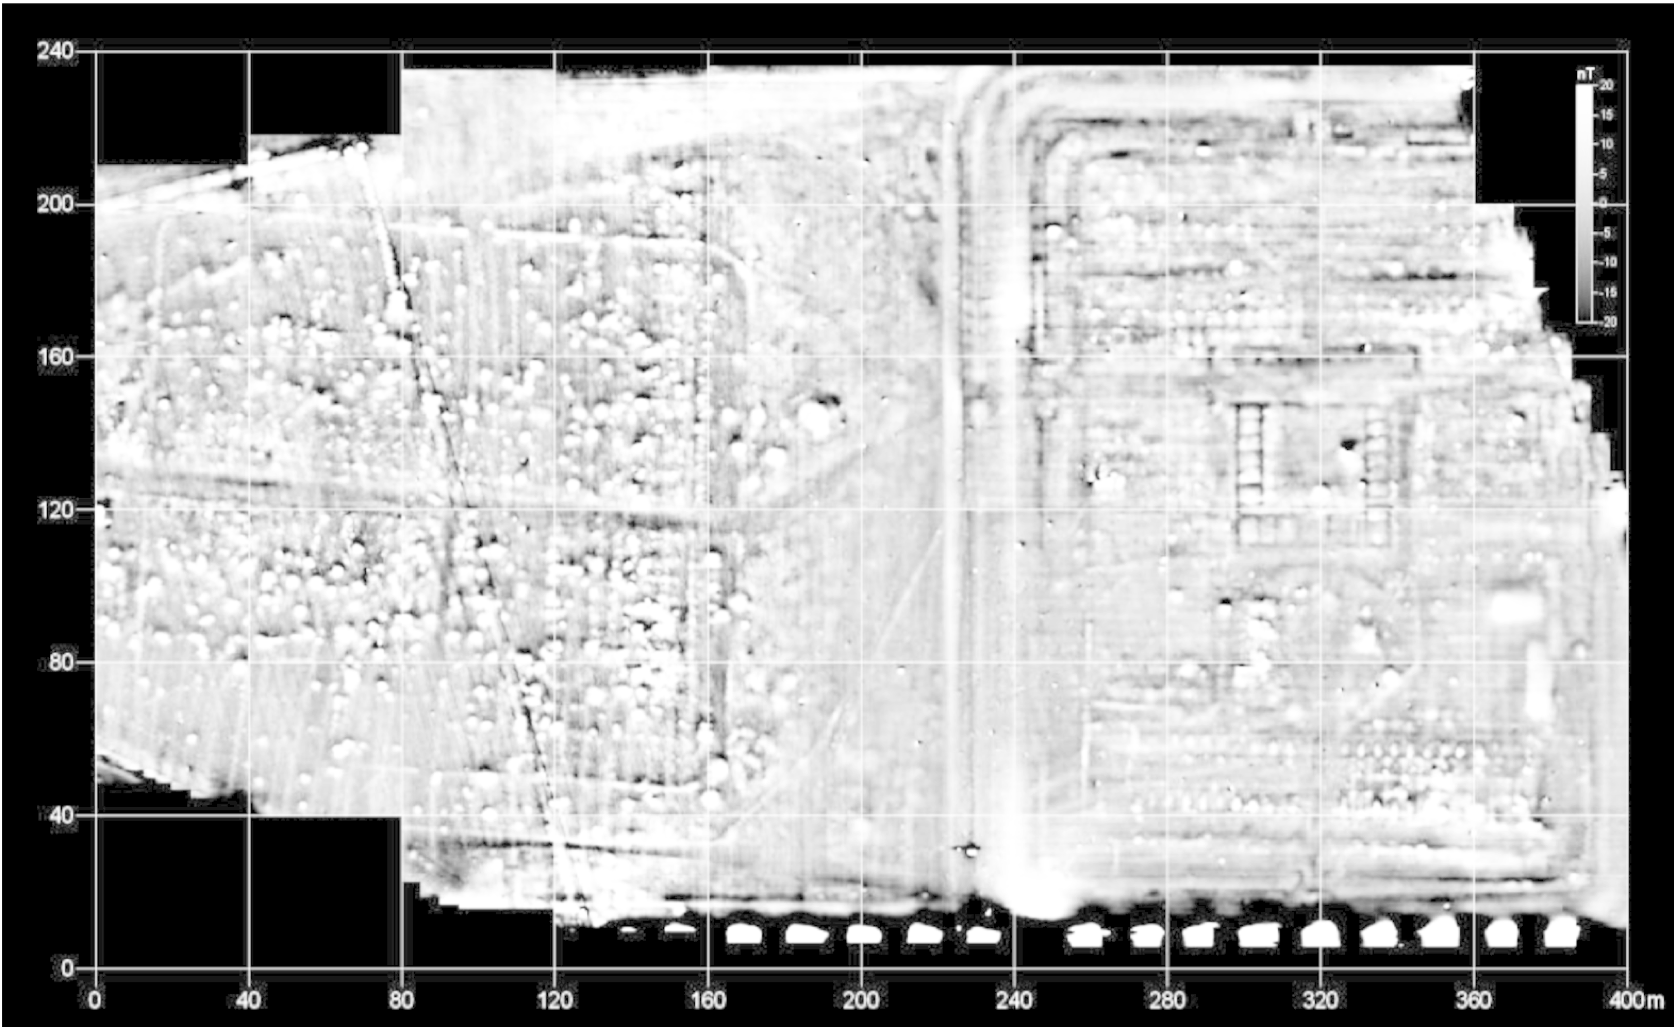
\includegraphics[width=0.99\textwidth]{Figures/General/GeophysExamples/Magnetics1_FassbinderBADS.png}
        \tiny[Fassbinder, Bavarian Academy of Sciences]
           \end{PointSix}
\end{frame}
\begin{frame}
    \begin{PointSix}{Example: Magnetics}
        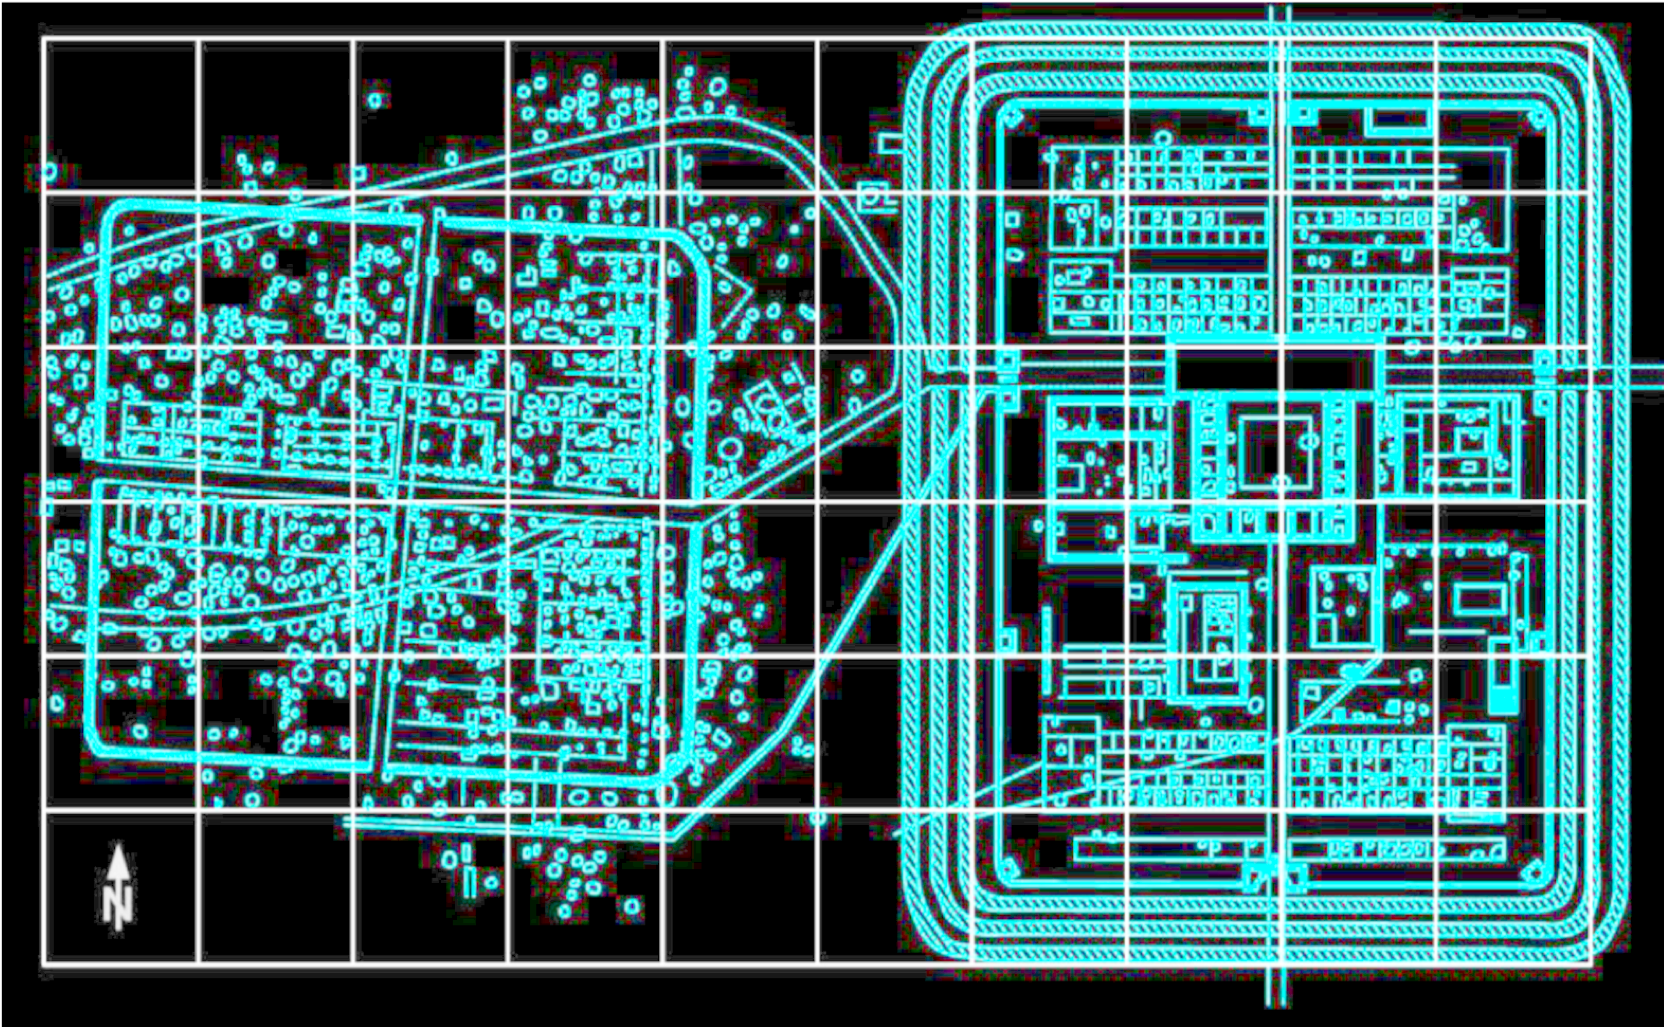
\includegraphics[width=0.99\textwidth]{Figures/General/GeophysExamples/Magnetics2_FassbinderBADS.png}
        \tiny[Fassbinder, Bavarian Academy of Sciences]
           \end{PointSix}
\end{frame}
\begin{frame}
    \begin{PointSix}{Example: Geoelectrics}
        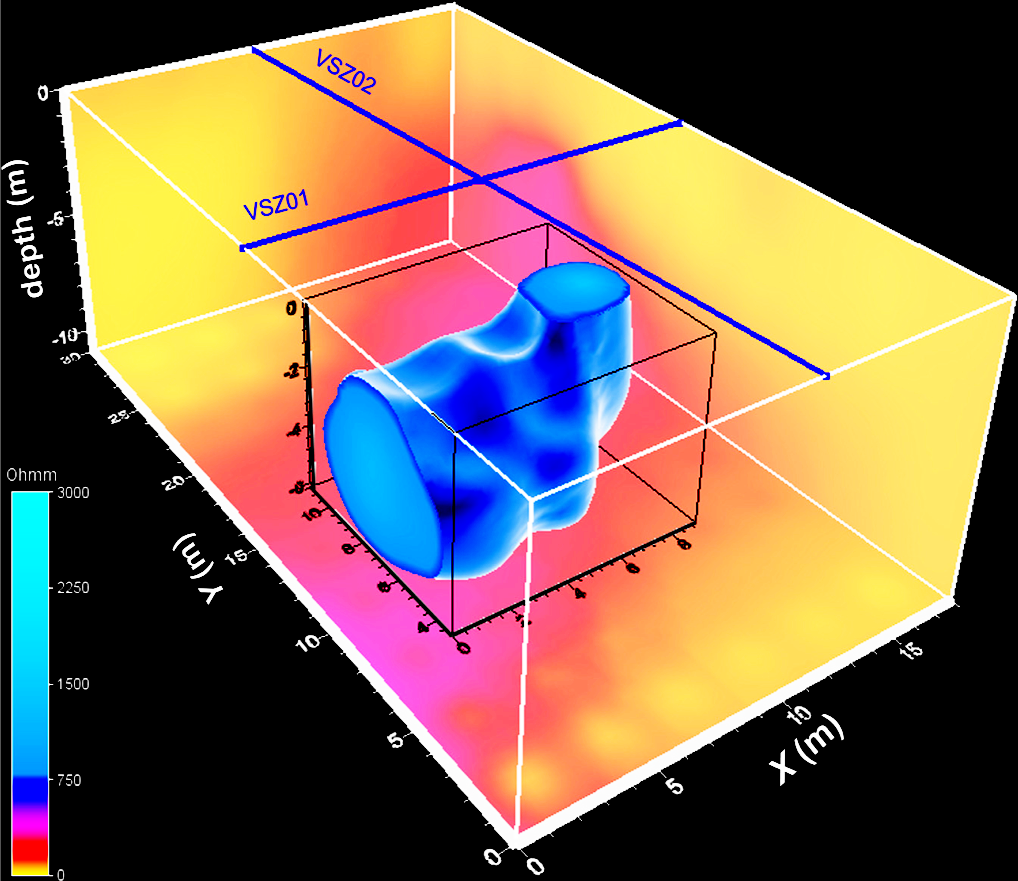
\includegraphics[width=0.9\textwidth]{Figures/General/GeophysExamples/DCElectricsSinkhole_Plank2019NearSurfaceGeophys_Reversed.png}

        \tiny[Plank et al., Near Surface Geophysics, 2019]
        %Volumetric interpretation of the former sinkhole at 900 Ωm isovalue. The resistivity scale is not artificially distorted. The yellow lines indicate the traces of 2D geoelectric survey lines. The crossing point is not above the sinkhole.
        \end{PointSix}
\end{frame}

\begin{frame}
    \begin{PointSix}{Example: Gravity}
        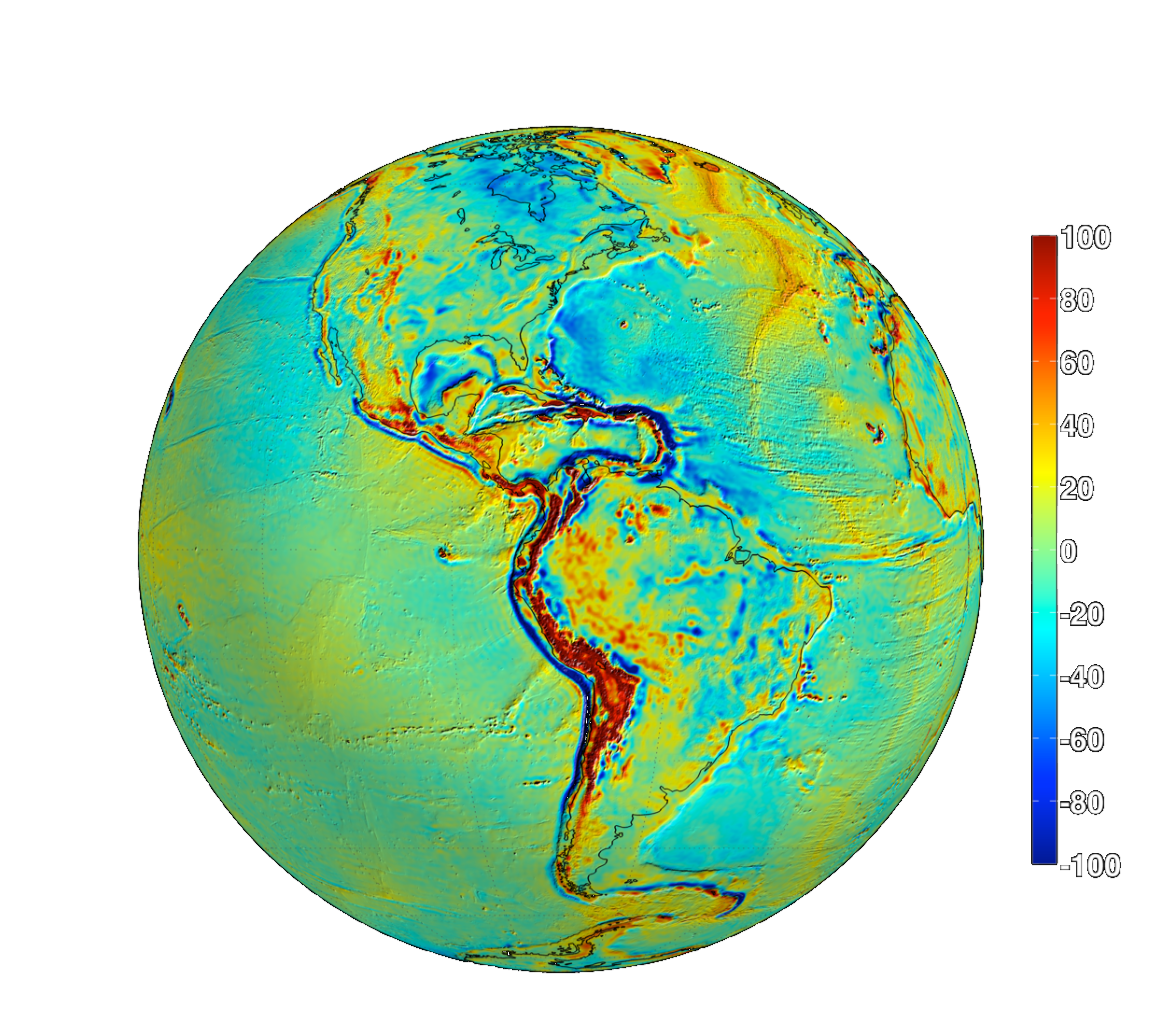
\includegraphics[width=0.90\textwidth]{Figures/Gravity/Exported/Grace_JPLCaltect_FODT10_WithoutPeople.png}
    \end{PointSix}
\end{frame}



\begin{frame}
    \small
    \begin{PointSix}{How do we teach? }
        \begin{itemize}
            \item Video Lectures or Plenum (Tuesdays)
            \item Exercises \& 1-1-Interaction (Thursdays)
            \item Applied Exercises (Magnetics, Electrics, Seismics)
        \end{itemize}
    \end{PointSix}
\end{frame}

\begin{frame}
    \begin{PointSix}{How do we teach?}
        \small
        \alert{Learning Goals}
        \begin{itemize}
            \item Obtain a broad overview of geophysical methods for sub-surface imaging.
            \item Understand the underlying physical principles.
            \item Learn how to think logically \& quantitatively.
        \end{itemize}
    \end{PointSix}
\end{frame}

\begin{frame}
    \begin{PointThree}{How do we teach?}
        \small
        \alert{Expectations}
        \begin{itemize}
            \item Be prepared.
            \item Ask questions.
            \item Do the work.
        \end{itemize}
    \end{PointThree}
\end{frame}

\begin{frame}
    \begin{PointSix}{How do we teach? $\rightarrow$ Ilias}
        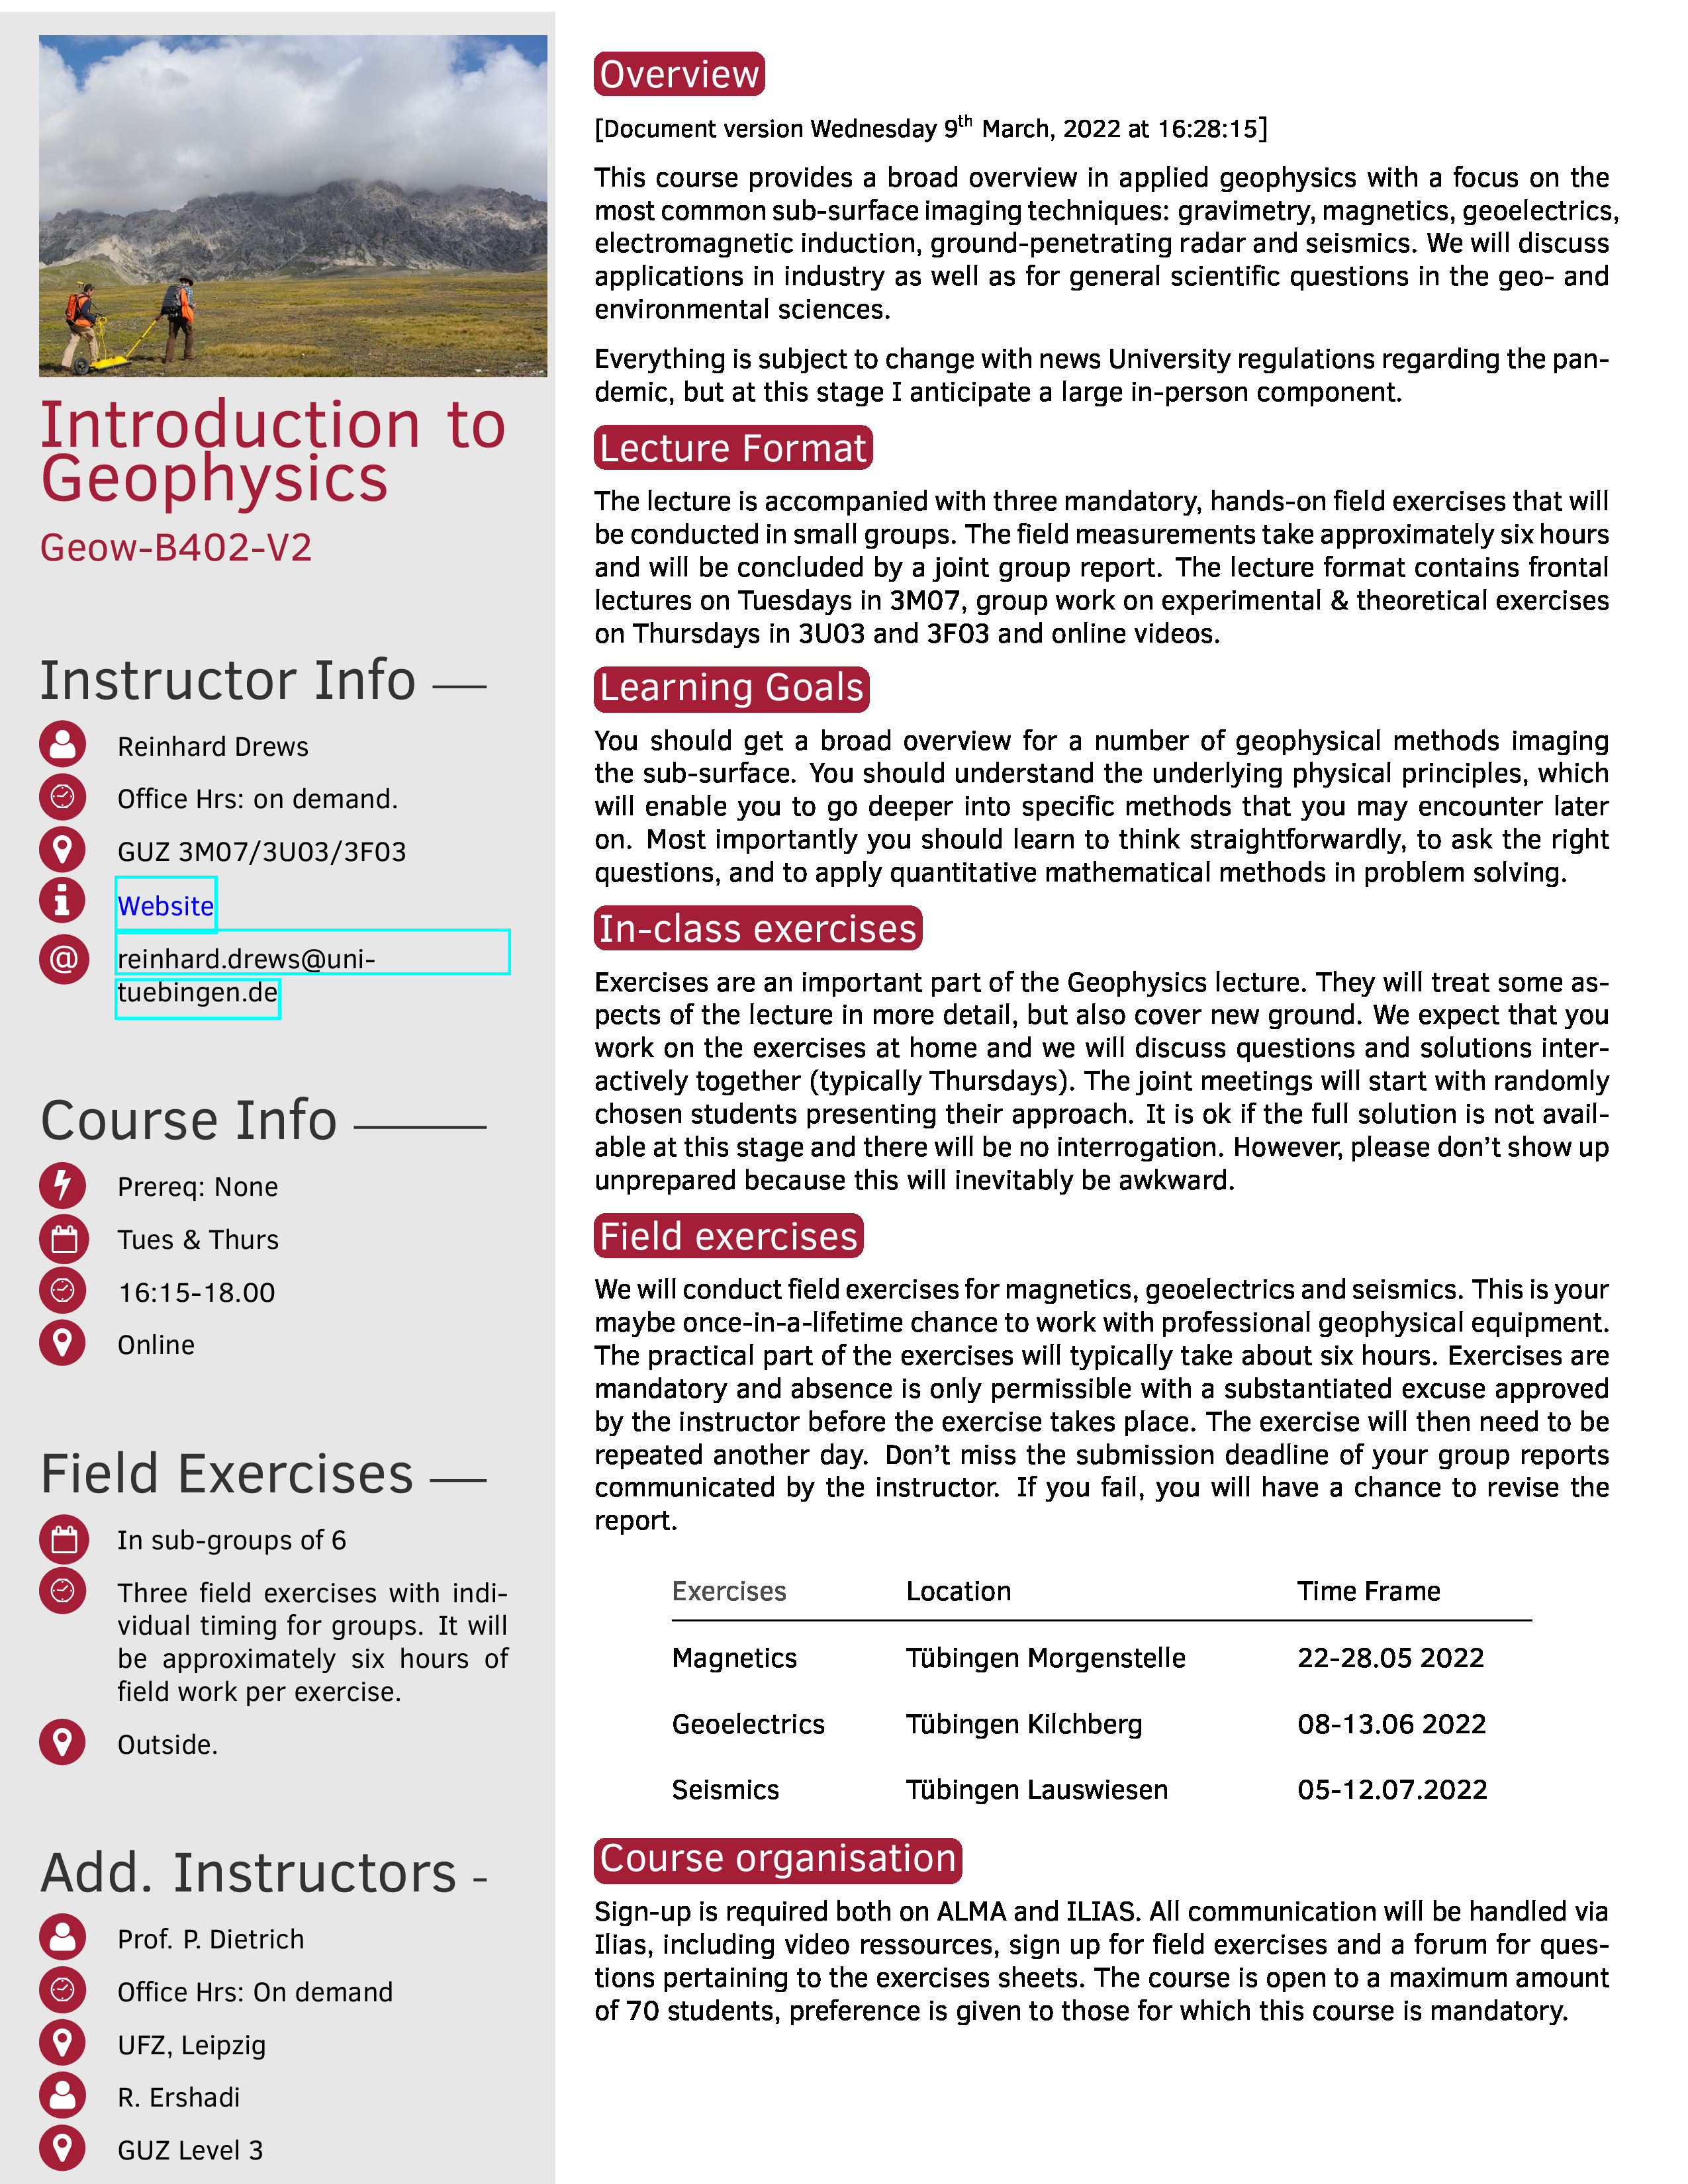
\includegraphics[width=0.90\textwidth]{Figures/General/LectureOutline_PageOne.jpg}
    \end{PointSix}
\end{frame}
%\begin{frame}
  \begin{PointSix}{Learning Goals}
    \alert{Learning goals today:}
    \begin{itemize}
      \item The gravitational force, its potential field, and how to measure it.
      \item The reference gravitational field of the Earth.
    \end{itemize}
  \end{PointSix}
  \end{frame}

\begin{frame}
  \begin{PointSix}{Example: Global variability}
      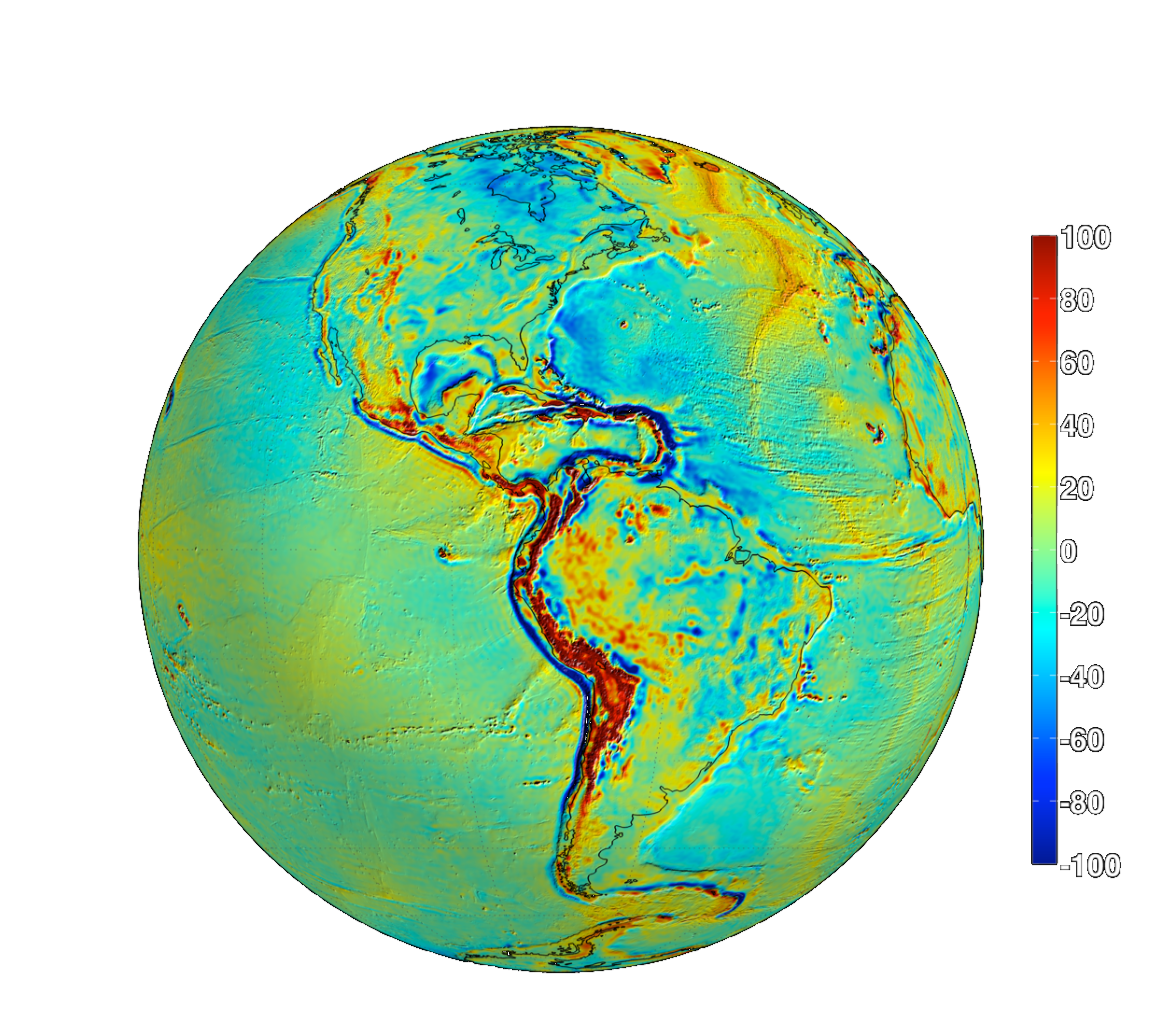
\includegraphics[width=0.99\textwidth]{Figures/Gravity/Exported/Grace_JPLCaltect_FODT10_WithoutPeople.png}
  \end{PointSix}
\end{frame}

\begin{frame}
  \begin{PointSix}{Example: Global variability}
  \centering
  \small Your mass is constant but your weight is not.
  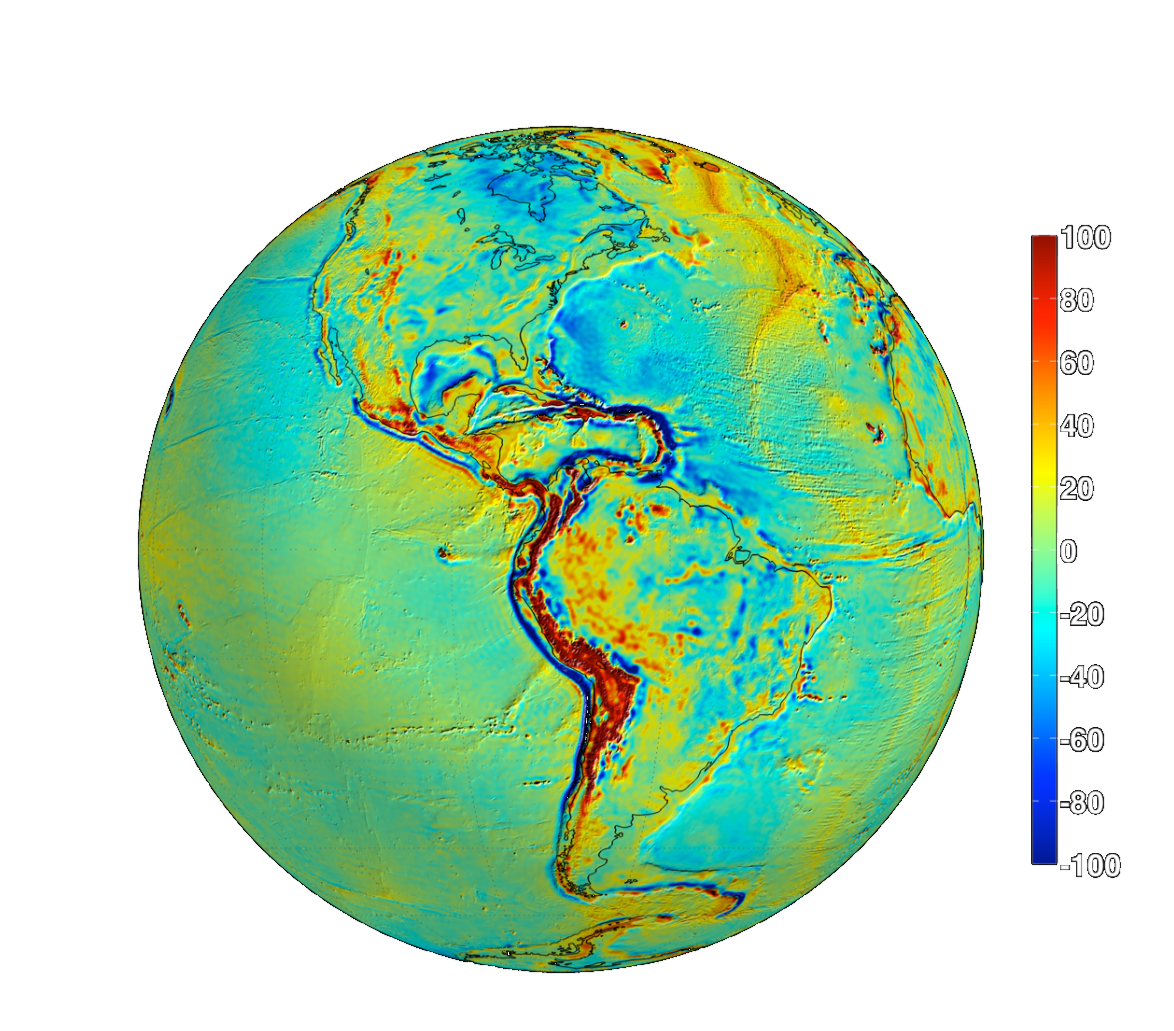
\includegraphics[width=0.99\textwidth]{Figures/Gravity/Exported/Grace_JPLCaltect_FODT10_WithPeople.png}
  \end{PointSix}
\end{frame}


\begin{frame}
\begin{ThreeCols}{What is a force?}{
  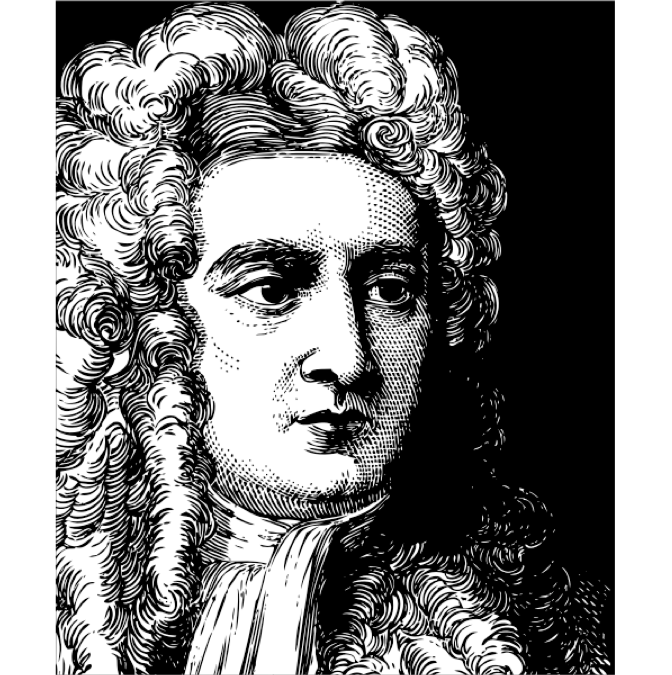
\includegraphics[width=0.8\textwidth]{Figures/Gravity/Exported/Newton_PD_GJohnson.png} \centering \tiny [Newton (1642-1726) / G. Johnson.]}
  \scalebox{1.5}{%
      $
      \vec{F} = m \vec{g}
      $
  }
  \scalebox{0.6}{\parbox{\linewidth}{
      \begin{align*}
      &\vec{F}:\,\text{Force}\,(\text{N};\,\text{kg}\,\text{m}\,\text{s}^{-2})\\
      &\vec{g}:\,\text{Acceleration}\,(\text{m}\,\text{s}^{-2})\\
      &\text{m}:\,\text{Mass (kg)}
      \end{align*}
  }}
\end{ThreeCols}
\end{frame}

\begin{frame}
  \begin{ThreeCols}{The gravitational force}{
      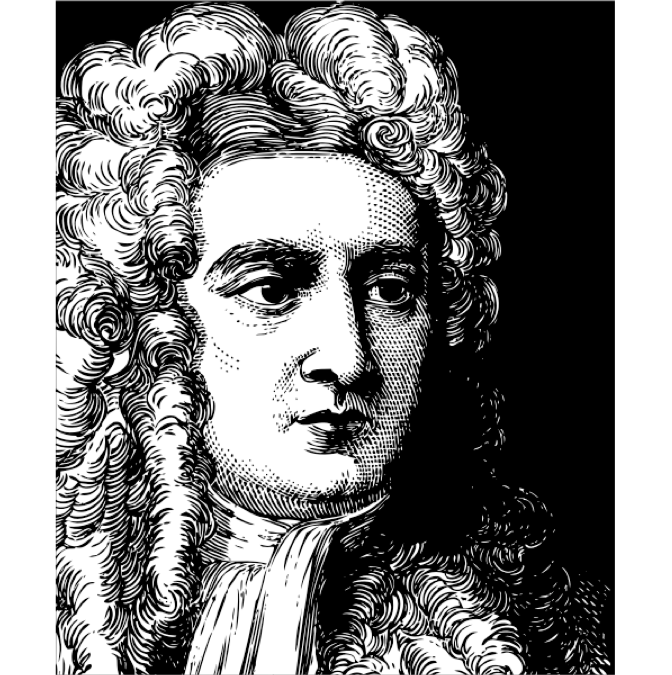
\includegraphics[width=0.8\textwidth]{Figures/Gravity/Exported/Newton_PD_GJohnson.png} \centering \tiny [Newton (1642-1726) / G. Johnson.]}
      \scalebox{1.5}{%
          $
          \vec{F} = G\frac{mM}{r^2}\hat{r}
          $
      }
      \scalebox{0.6}{\parbox{\linewidth}{
          \begin{align*}
          &G=6.674 \cdot 10^{-11}\,\text{(}\,m^3 kg^{-1} s^{-2}\text{)}\\
          &\hat{r}:\,\text{unit vector}\\
          &r:\,\text{distance between point masses}
          \end{align*}
      }}
      \begin{tikzpicture}
          \coordinate (A) at (1,2);
          \coordinate (B) at (2,4);

          \draw [fill=white] (A) circle (8pt) node [left,xshift=-0.5cm] {M};
          \draw [fill=white] (B) circle (4pt) node [left,xshift=-0.5cm] {m};


          \draw[-latex,thick,Karminrot,->] (A) -- (B) node[midway,left,rotate=0] {$r$};
          \draw [-latex,thick, Karminrot] (B) -- (A);
          \end{tikzpicture}
  \end{ThreeCols}
  \end{frame}

  \begin{frame}
      \begin{PointSix}{Example: The gravitational constant}
          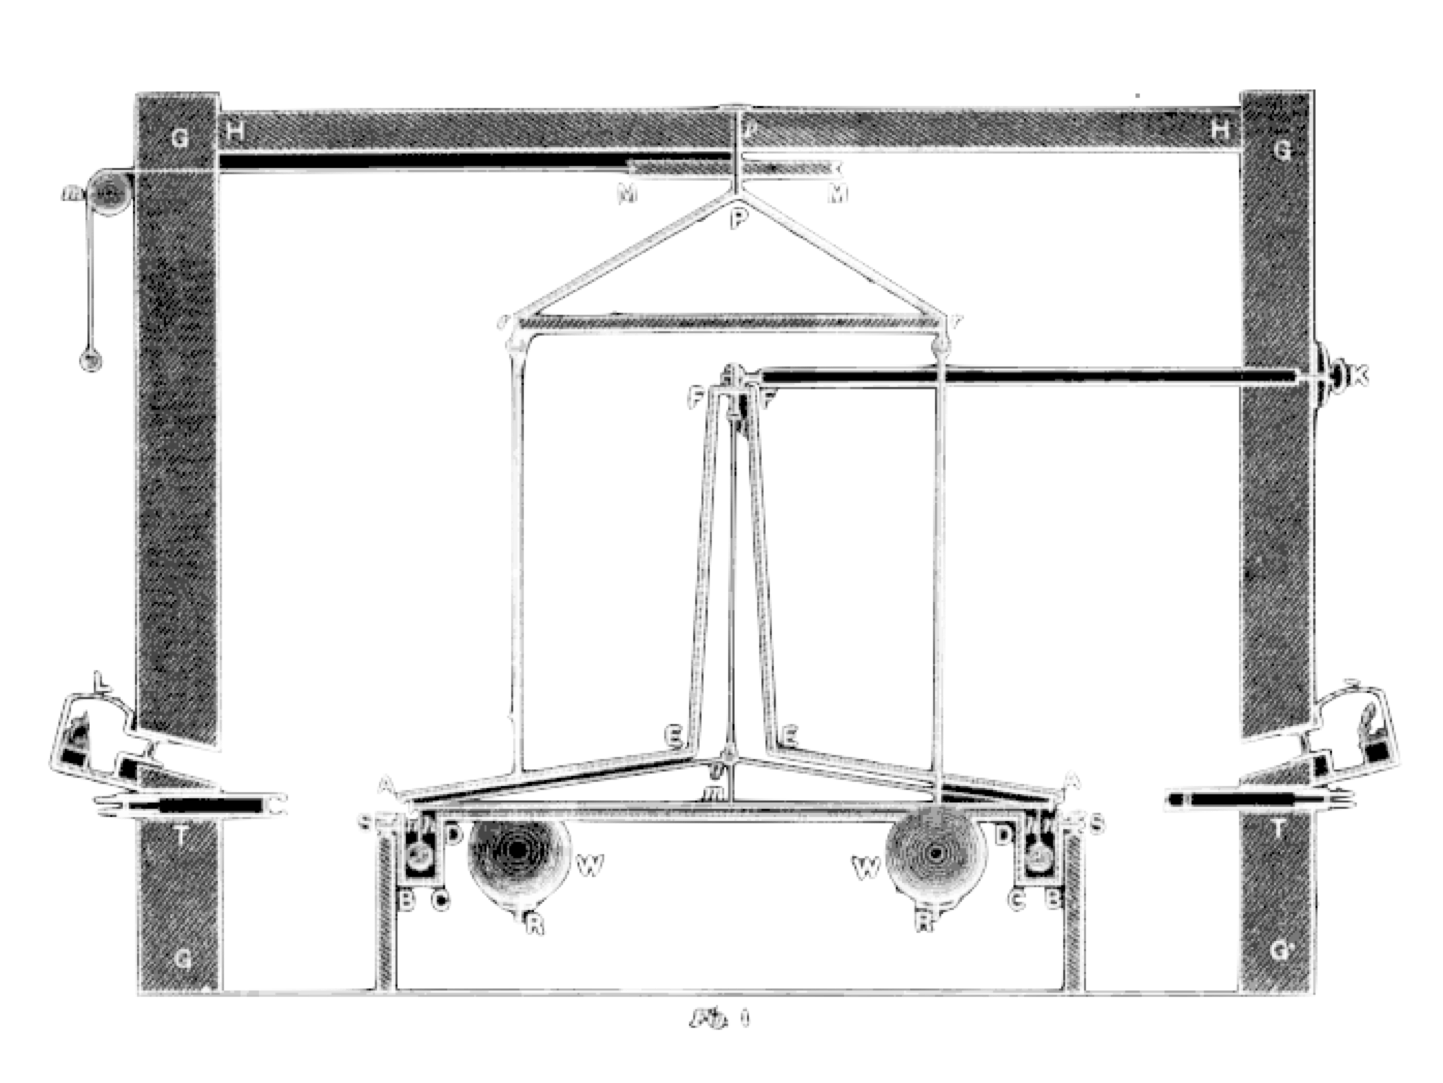
\includegraphics[width=0.99\textwidth]{Figures/Gravity/Exported/Cavendish_PNAS1798.png}
          \centering
          \tiny Cavnedish, PNAS, 1798
      \end{PointSix}
  \end{frame}
  \begin{frame}
      \begin{PointSix}{Example: The gravitational constant}
          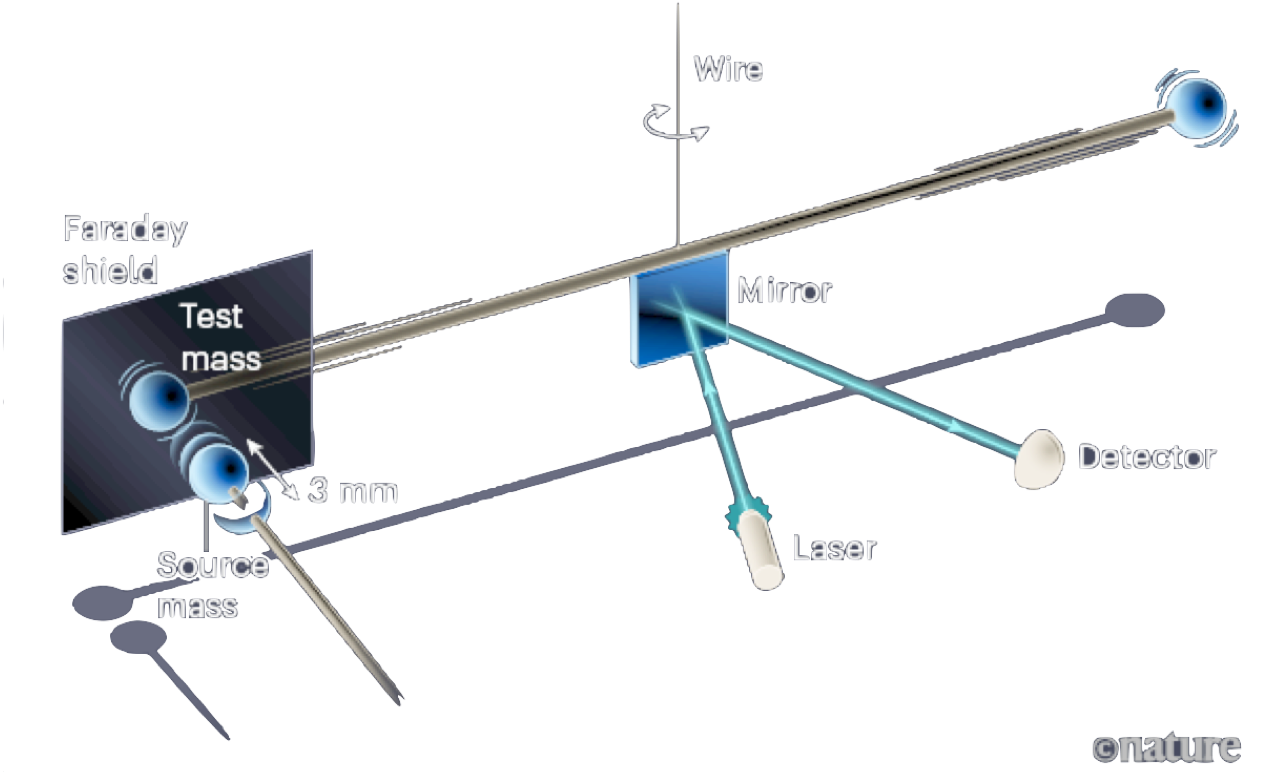
\includegraphics[width=0.99\textwidth]{Figures/Gravity/Exported/MeasuringG_Westphal_Nature2021.png}
          \centering
          \tiny Westphal et al., Nature, 2021\\
          \normalsize G is the worst known constant in physics. Why?
      \end{PointSix}
  \end{frame}

\begin{frame}
\begin{PointSix}{Example: Measuring acceleration}
  \begin{minipage}[t]{0.3\textwidth}
    
\includegraphics[width=\textwidth]{Figures/General/ScarySmiley_Kindpng.png}
    \end{minipage}\begin{minipage}[]{0.7\textwidth}
  \centering
  \begin{align*}
  &\vec{F} = m \vec{g} \\
  &\vec{F} = G\frac{mM}{r^2}\hat{r} \\
  &\rightarrow \vec{g} = G\frac{M}{r^2}\hat{r} \\
  &\rightarrow \frac{d^2\vec{x}}{dt^2} = G\frac{M}{r^2}\hat{r} \\
  \end{align*}
\end{minipage}
  \centering
  This is a differential equation.

\end{PointSix}
\end{frame}

\begin{frame}
\begin{PointSix}{Example: Measuring acceleration}
  \begin{minipage}[t]{0.3\textwidth}
    
\includegraphics[width=\textwidth]{Figures/General/IcandothisSmiley_Kindpng.png}
    \end{minipage}\begin{minipage}[]{0.7\textwidth}
  \centering
  \begin{align*}
  &\frac{d^2\vec{x}}{dt^2} = G\frac{M}{R_E^2} \approx const. \\
  \end{align*}
\end{minipage}
 % \centering
  At the Earth's surface ($R_E$) g is close to constant and only vertical. (Later we will see that none of this is not quite true).

\end{PointSix}
\end{frame}

\begin{frame}
  \begin{PointSix}{Example: Measuring acceleration}
  \begin{tikzpicture}
      \begin{axis}[
        rdstyle,
        xlabel=time (s),
        ylabel={$g (m s^{-2})$},
        xmin=0,
        xmax=10,
        xtick={0,2,...,10},
        color=white,
        width=9cm,
      ]
        \addplot[domain=0:10,samples=10,color=Karminrot,line width=0.5mm] {x*0 +9.81};
        \node[] at (axis cs: 5,11) {$g = \frac{d^2}{dt^2}x(t)=\frac{GM}{R_e^2}\approx const.$};
      \end{axis}
    \end{tikzpicture}
  \end{PointSix}
\end{frame}

\begin{frame}
  \begin{PointSix}{Example: Measuring acceleration}
  \begin{tikzpicture}
      \begin{axis}[
        rdstyle,
        xlabel=time (s),
        ylabel={$v (m s^{-1})$},
        xmin=0,
        xmax=10,
        xtick={0,2,...,10},
        ytick=9.81,
        yticklabels={$c_1$},
        color=white,
        width=9cm,
      ]
        \addplot[domain=0:10,samples=10,color=Karminrot,line width=0.5mm] {x + 9.81};
        \node[] at (axis cs: 5,20) {$v = \int g dt=\frac{d}{dt}x(t)=\frac{GM}{R_e^2}t+c_1$};
      \end{axis}
    \end{tikzpicture}
  \end{PointSix}
\end{frame}

\begin{frame}
  \begin{PointSix}{Example: Measuring acceleration}
  \begin{tikzpicture}
      \begin{axis}[
        rdstyle,
        xlabel=time (s),
        ylabel={$x (m)$},
        xmin=0,
        xmax=10,
        xtick={0,2,...,10},
        ytick=9.81,
        yticklabels={$c_2$},
        color=white,
        width=9cm,
      ]
        \addplot[domain=0:10,samples=10,color=Karminrot,line width=0.5mm] {x^2 + 10};
        \node[] at (axis cs: 5,100) {$x(t) = \int v(t) dt=\frac{GM}{2R_e^2}t^2+c_1t+c_2$};
      \end{axis}
    \end{tikzpicture}
  \end{PointSix}
\end{frame}
\begin{frame}

\begin{PointSix}{Example: Measuring acceleration}
     \begin{align*}
       & x(t) = \frac{GM}{2R_e^2}t^2+c_1t+c_2 \\
     \end{align*}
     \begin{itemize}
      \item Setting, e.g., $c1=0$ (initial velocity) and $c_2=0$ (initial position) is quite convenient.
      \item This is the principal of a free-fall gravimeter.
    \end{itemize}
\end{PointSix}

\end{frame}

\begin{frame}
\begin{PointSix}{Exercises: Group-Work Thursdays}
  \begin{itemize}
    \item Thanks to the Greeks we know the radius $R_E$ for the Earth. However, its mass was unknown for a while.
    \item Go ahead and determine the mass of the Earth M with your Smartphone!
    \item \alert{There is an important first-order finding in Earth Sciences that you can (re-) discover. Which one?}
  \end{itemize}

\end{PointSix}
\end{frame}

\begin{frame}
\begin{PointSix}{Beyond point masses}
  \begin{tikzpicture}
    \coordinate (A) at (8,0);
    \coordinate (B) at (4,-3.5);
    \coordinate (C) at (5,-3.5);
    \coordinate (D) at (6,-3.5);
    \draw [thick] (0,0.0) -- (8,0.0);
    % drawing the node with shape=rectangle and anchor=center
    \node [draw, Karminrot, thick, shape=rectangle, minimum width=0.25cm, minimum height=0.25cm, anchor=center] at (B) {};
    \draw [->, thick] (0,0.0) -- (B) node[xshift=0.3cm,yshift=0.3cm,midway,left,rotate=-30] {$\vec{r}$};;

    \node[yshift=0.3cm] at (A) {\small Surface};

  \end{tikzpicture}
  $$
    \vec{F} = G\frac{dM}{r^2}\hat{r}
  $$
\small For a small mass dM the point mass approximation holds.
\end{PointSix}

\end{frame}



\begin{frame}
\begin{PointSix}{Beyond point masses}
  \begin{tikzpicture}
    \coordinate (A) at (8,0);
    \coordinate (B) at (4,-3.5);
    \coordinate (C) at (5,-3.5);
    \coordinate (D) at (6,-3.5);
    \draw [thick] (0,0.0) -- (8,0.0);
    % drawing the node with shape=rectangle and anchor=center
    \node [draw, Karminrot, thick, shape=rectangle, minimum width=0.25cm, minimum height=0.25cm, anchor=center] at (B) {};
    \foreach \i in {0,2,...,8}
    {
      \draw [->, thick] (0+\i,0.0) -- (B);
    }
    \node[yshift=0.3cm] at (A) {\small Surface};

  \end{tikzpicture}
  $$
    \vec{F} = G\frac{dM}{r^2}\hat{r}
  $$
  \small Profiling across a sub-surface target results in a gravity anomaly ($\rightarrow$ Exercises).
\end{PointSix}
\end{frame}

\begin{frame}
\begin{PointSix}{Beyond point masses}
  \begin{tikzpicture}
    \coordinate (A) at (8,0);
    \coordinate (B) at (4,-3.5);
    \coordinate (C) at (5,-3.5);
    \coordinate (D) at (6,-3.5);
    \draw [thick] (0,0.0) -- (8,0.0);
    \node[yshift=0.3cm] at (A) {\small Surface};

    \foreach \i in {-2,-1.5,...,2}
    {
      \foreach \j in {0,0.5}
      {
        \node [draw, Karminrot, thick, shape=rectangle, minimum width=0.25cm, minimum height=0.25cm, anchor=center] at (4-\i,-3.5-\j) {};
        \draw [->, thick] (0,0.0) -- (4-\i,-3.5-\j) ;

      }
    }

  \end{tikzpicture}
  $$
  \vec{F}(\vec{r}) = \sum_i G\frac{dM_i}{r_i^2}\hat{r_i}
  $$
  \small For $i$ point masses the effect adds up.
\end{PointSix}
\end{frame}

\begin{frame}
\begin{PointSix}{Beyond point masses}
  \begin{tikzpicture}
    \coordinate (A) at (8,0);
    \coordinate (B) at (4,-3.5);
    \coordinate (C) at (5,-3.5);
    \coordinate (D) at (6,-3.5);
    \draw [thick] (0,0.0) -- (8,0.0);
    \node[yshift=0.3cm] at (A) {\small Surface};

    \foreach \i in {-2,-1.5,...,2}
    {
      \foreach \j in {0,0.5}
      {
        \node [draw, Karminrot, thick, shape=rectangle, minimum width=0.25cm, minimum height=0.25cm, anchor=center] at (4-\i,-3.5-\j) {};
        \draw [->, thick] (2,0.0) -- (4-\i,-3.5-\j) ;

      }
    }
  \end{tikzpicture}
  $$
    \vec{F}(\vec{r}) = \sum G\frac{dM_i}{r_i^2}\hat{r_i}
  $$
\end{PointSix}

\end{frame}

\begin{frame}
\begin{PointSix}{Beyond point masses}
  \begin{tikzpicture}
    \coordinate (A) at (8,0);
    \coordinate (B) at (4,-3.5);
    \coordinate (C) at (5,-3.5);
    \coordinate (D) at (6,-3.5);
    \draw [thick] (0,0.0) -- (8,0.0);
    \node[yshift=0.3cm] at (A) {\small Surface};
    \foreach \i in {-2,-1.5,...,2}
    {
      \foreach \j in {0,0.5}
      {
        \node [draw, Karminrot, thick, shape=rectangle, minimum width=0.25cm, minimum height=0.25cm, anchor=center] at (4-\i,-3.5-\j) {};
        \draw [->, thick] (4,0.0) -- (4-\i,-3.5-\j) ;

      }
    }
  \end{tikzpicture}
  $$
  \vec{F}(\vec{r}) = \sum G\frac{dM_i}{r_i^2}\hat{r_i}
  $$
\end{PointSix}
\end{frame}


\begin{frame}
\begin{PointSix}{Beyond point masses}
  \begin{tikzpicture}
    \coordinate (A) at (8,0);
    \coordinate (B) at (4,-3.5);
    \coordinate (C) at (5,-3.5);
    \coordinate (D) at (6,-3.5);
    \draw [thick] (0,0.0) -- (8,0.0);
    \node[yshift=0.3cm] at (A) {\small Surface};

    \foreach \i in {-2,-1.5,...,2}
    {
      \foreach \j in {0,0.5}
      {
        \node [draw, Karminrot, thick, shape=rectangle, minimum width=0.25cm, minimum height=0.25cm, anchor=center] at (4-\i,-3.5-\j) {};
        \draw [->, thick] (7,0.0) -- (4-\i,-3.5-\j) ;

      }
    }
  \end{tikzpicture}
  $$
  \vec{F}(\vec{r}) = \sum G\frac{dM_i}{r_i^2}\hat{r_i}
  $$
\end{PointSix}
\end{frame}


\begin{frame}
\begin{PointSix}{Beyond point masses}
  \begin{tikzpicture}
    \coordinate (A) at (8,0);
    \coordinate (B) at (4,-3.5);
    \coordinate (C) at (5,-3.5);
    \coordinate (D) at (6,-3.5);
    \draw [thick] (0,0.0) -- (8,0.0);
    \node[yshift=0.3cm] at (A) {\small Surface};
    \node[yshift=-1.8cm,xshift=-4cm] at (A) {$\vec{F}(\vec{r}) = G \int \rho \frac{1}{r^2}\hat{r}dV$};

    %
    \foreach \i in {-2,-1.5,...,2}
    {
      \foreach \j in {0,0.5}
      {
        \node [draw, Karminrot, thick, shape=rectangle, minimum width=0.25cm, minimum height=0.25cm, anchor=center] at (4-\i,-3.5-\j) {};
        %\draw [->, thick] (7,0.0) -- (4-\i,-3.5-\j) ;
      }
    }
    \node [draw, Karminrot, thick, shape=rectangle, minimum width=4.5cm, minimum height=1.25cm, anchor=center] at (4,-3.75) {};
  \end{tikzpicture}

  \only<1>{\small The summation can be replaced by an integration over a volume enclosing a continuous density.}\only<2>{\small The integration is a triple integral. Integration limits and coordinates depend on the viewpoint. Example is a Bouger plate, in general not easy to solve ($\rightarrow$ Exercises).}
    %\only<1>{The summation can be replaced by an integration over a volume enclosing a continuous density.} d $\rho$}\only<2>{Test,}d
\end{PointSix}
\end{frame}

\begin{frame}
\begin{PointSix}{Example: Shell}
  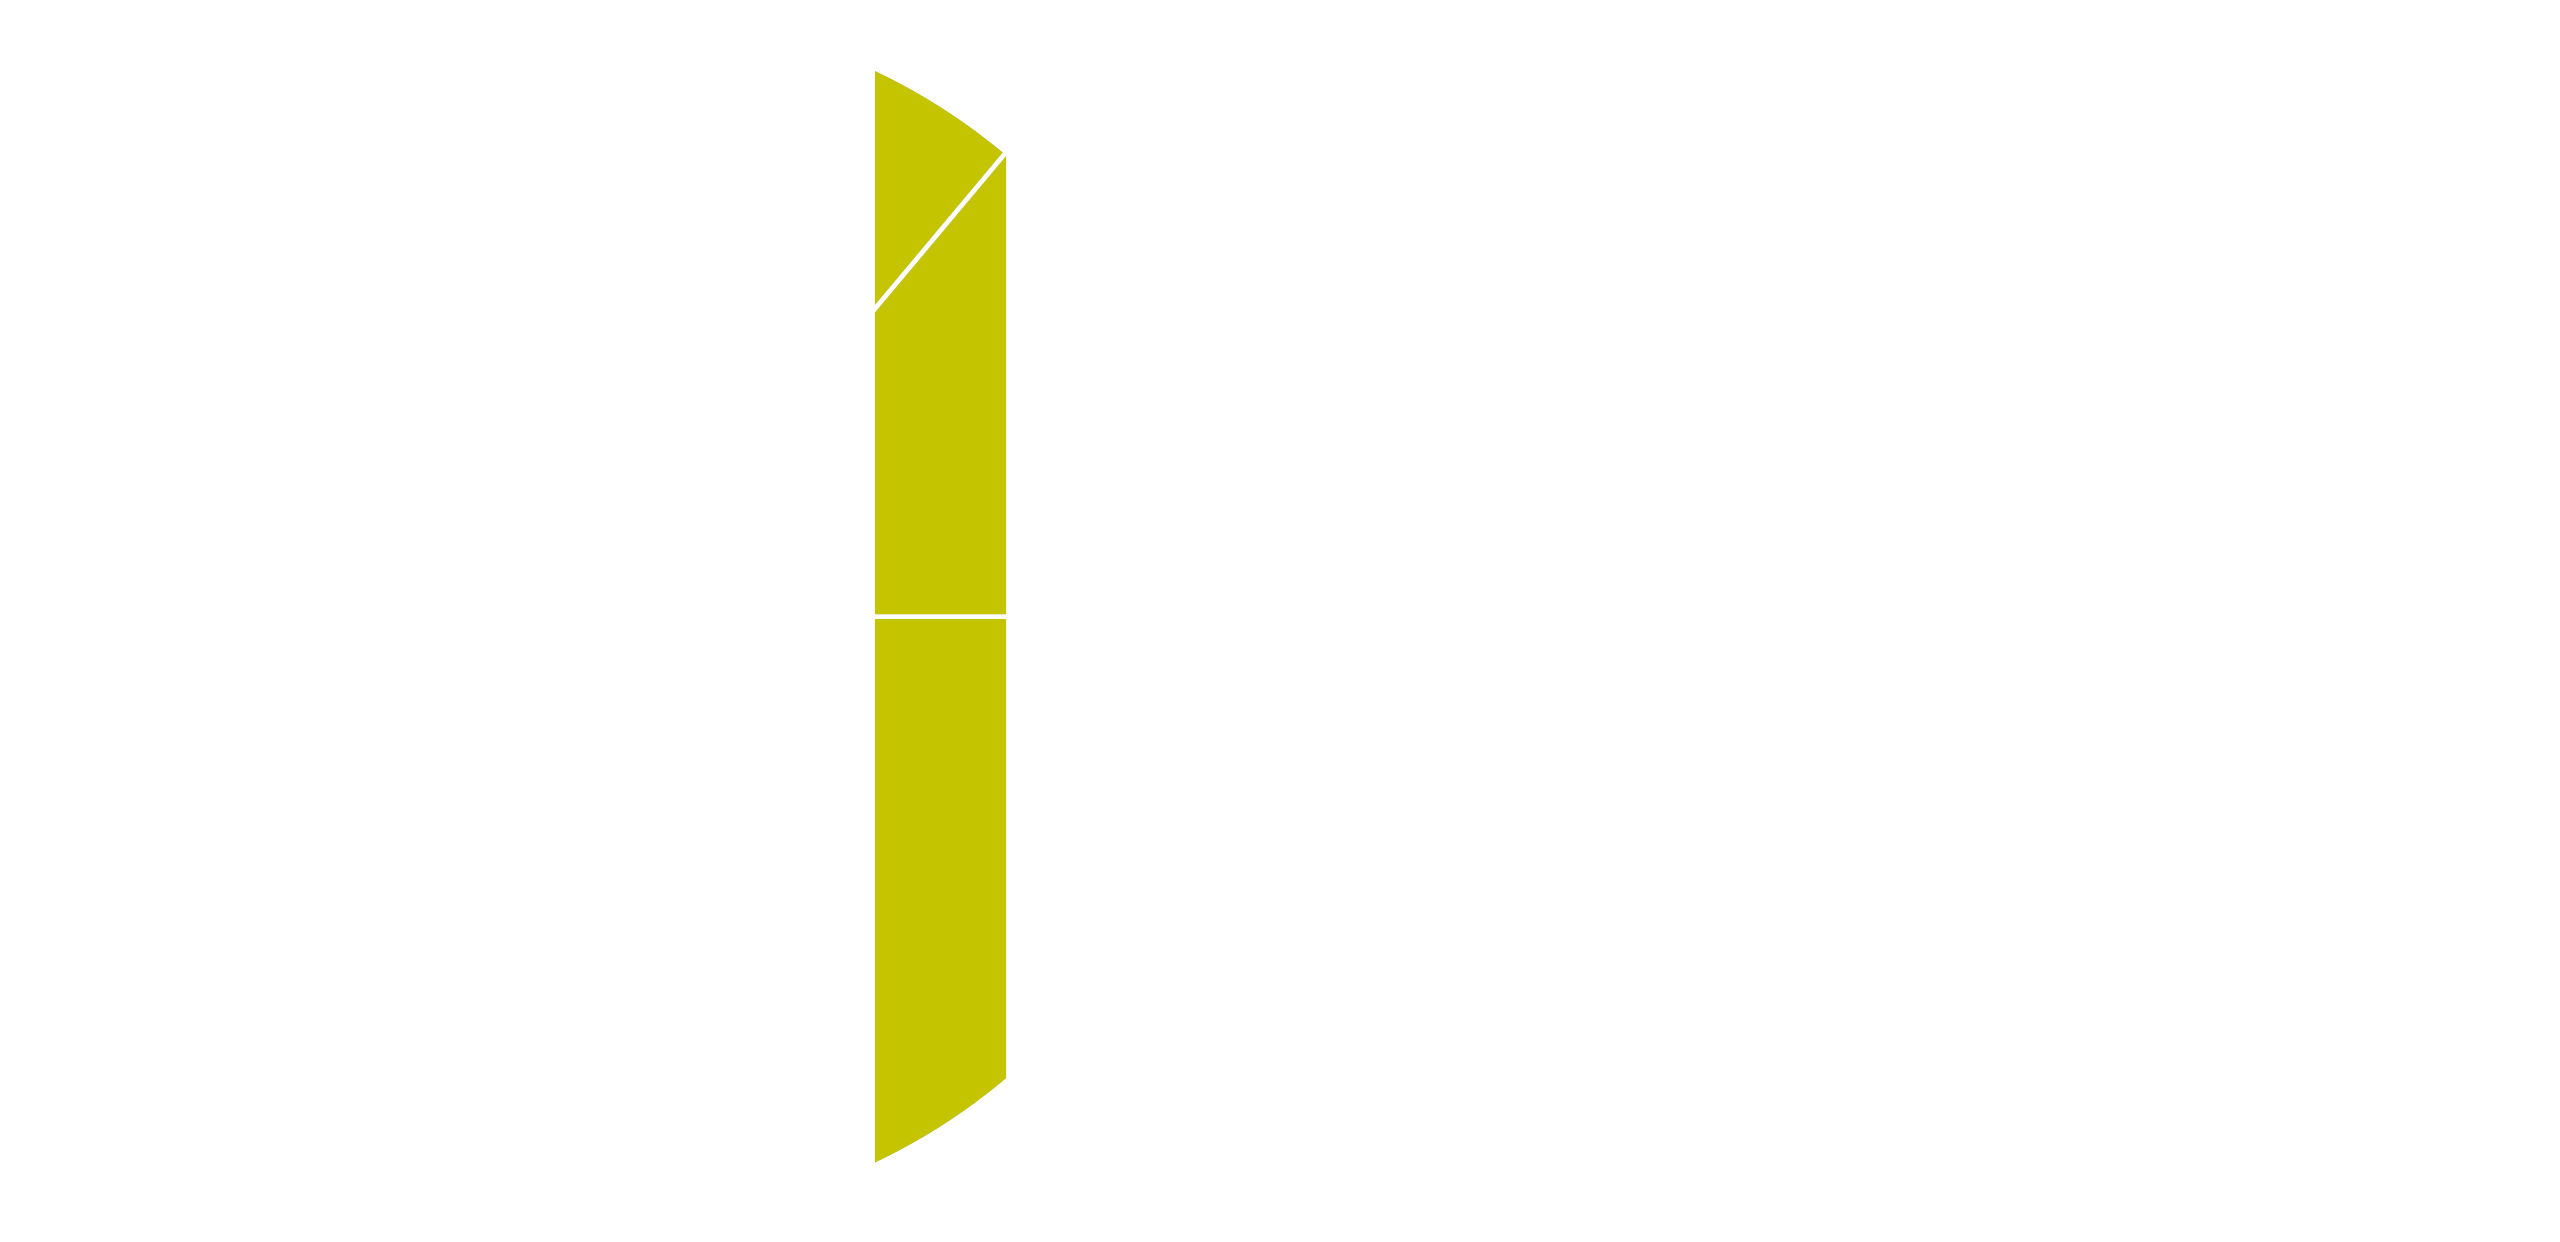
\includegraphics[width=0.99\textwidth]{Figures/Gravity/Exported/Shell-diag_reversed_CCBYSA4_0_Xaonon.png}
  \tiny [Xaononl CC BY-SA 4.0]

  \small Newton's shell theorem solves the volume integral inside and outside spherical objects ($\rightarrow$ Ex.-Discussion)
\end{PointSix}

\end{frame}

\begin{frame}
\begin{PointSix}{Newton's Shell Theorem}
 \begin{itemize}
    \item The field outside a shell is the same as the one from an equivalent point mass
    \item The field inside a shell is zero. Everywhere.
 \end{itemize}
\end{PointSix}
\end{frame}

\begin{frame}
\begin{PointSix}{Other shapes}
 \begin{itemize}
    \item \small There are analytical solutions for other shapes (e.g., Nagy 1966 for Prism).
 \end{itemize}
 \begin{center}
    \begin{tikzpicture}[>=latex,scale=2]

        \pgfmathsetmacro{\x}{1}
        \pgfmathsetmacro{\y}{1}
        \pgfmathsetmacro{\z}{1.5}
        \path (0,0,\y) coordinate (A) (\x,0,\y) coordinate (B) (\x,0,0) coordinate (C) (0,0,0)
        coordinate (D) (0,\z,\y) coordinate (E) (\x,\z,\y) coordinate (F) (\x,\z,0) coordinate (G)
        (0,\z,0) coordinate (H);
        \draw [thick] (-2,1.8) -- (3,1.8);
        \draw (A)--(B)--(C)--(G)--(F)--(B) (A)--(E)--(F)--(G)--(H)--(E);
        \draw (A)--(D)--(C) (D)--(H);
        \node[yshift=-0.3cm] at (2,1.8) {\small Surface};
        \draw[thin,|<->|] ($(A)+(0,-4pt)$) -- node[below]{x}($(B)+(0,-4pt)$);
        \draw[thin,|<->|] ($(B)+(-45:4pt)$) -- node[below,sloped]{y}($(C)+(-45:4pt)$);
        \draw[thin,|<->|] ($(C)+(4pt,0)$) -- node[below,sloped]{z}($(G)+(4pt,0)$);

    \end{tikzpicture}
\end{center}
\end{PointSix}
\end{frame}


\begin{frame}
\begin{PointSix}{Numerical forward modelling ($\rightarrow$ Ex)}
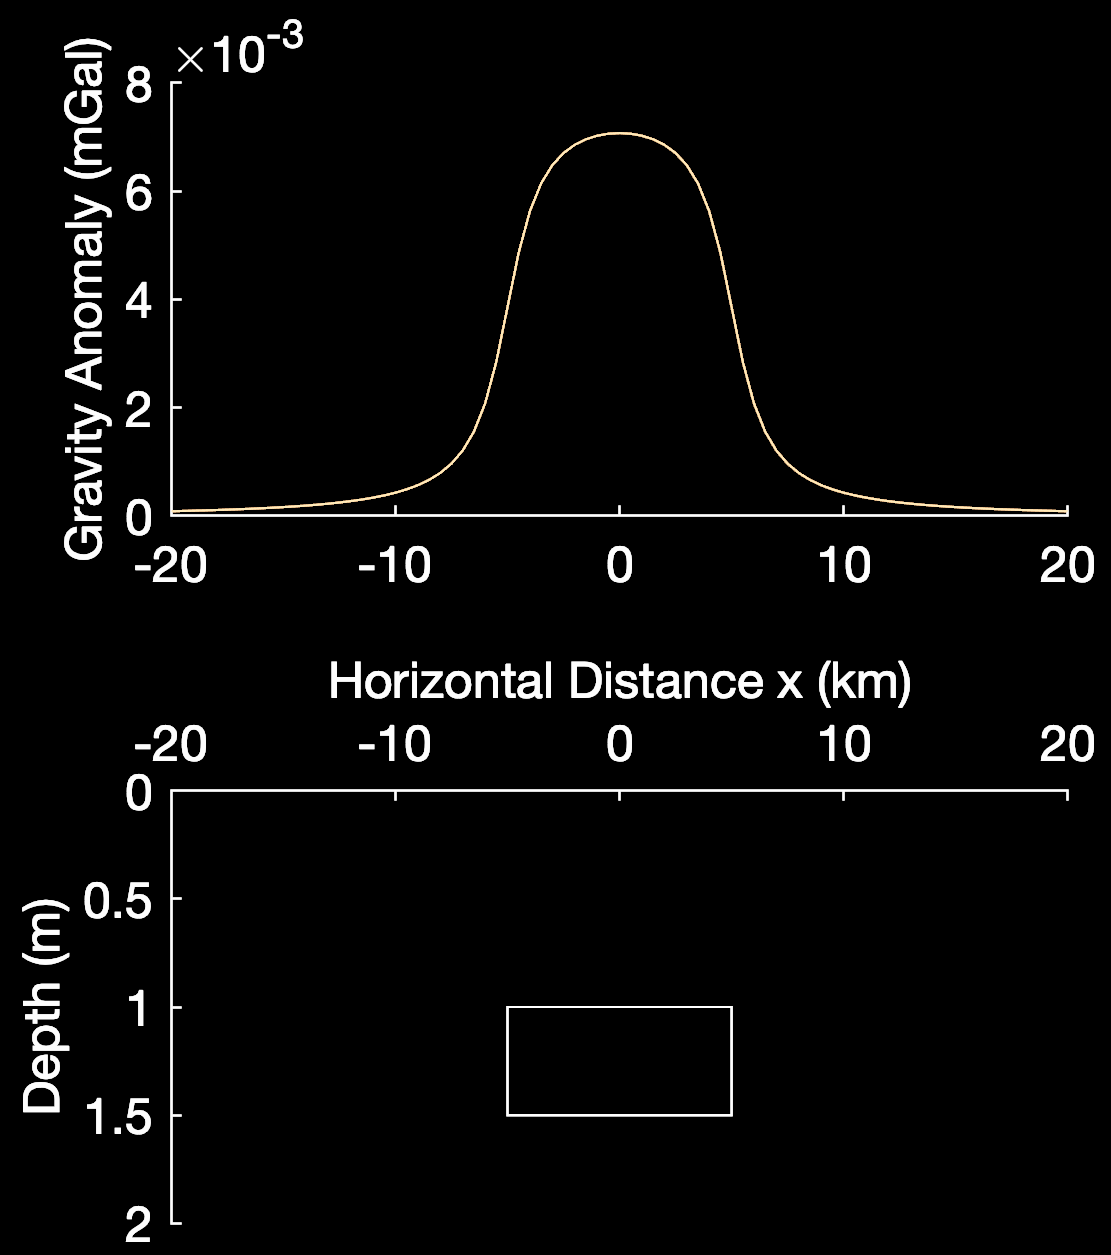
\includegraphics[width=0.8\textwidth]{Figures/Gravity/Exported/ForwardModelPrismReversed.png}
\end{PointSix}
\end{frame}



\begin{frame}
  \begin{PointSix}{Vector fields}
    \centering
    $
    \vec{g} = G\frac{M}{r^2}\hat{r}
    $
    \begin{center}
    \scalebox{0.85}{
        \begin{tikzpicture}
          \begin{axis}[
              xmin = -4, xmax = 4,
              ymin = -4, ymax = 4,
              zmin = 0, zmax = 1,
              axis equal image,
              xtick distance = 20,
              ytick distance = 20,
              view = {0}{90},
              scale = 1.25,
            % title = {\bf Vector Field $F = [-y,x]$},
              height=7cm,
            % xlabel = {$x$},
            % ylabel = {$y$},
              colormap/viridis,
            % colorbar,
            % colorbar style = {
            %     ylabel = {Vector Length}
            % }
            hide x axis,
            hide y axis,
          ]
          \addplot3[
                  point meta = {sqrt(x^2+y^2)},
                  quiver = {
                      u = {-x/sqrt(x^2+y^2)^2},
                      v = {-y/sqrt(x^2+y^2)^2},
                      scale arrows = 0.7,
                  },
                  quiver/colored = {mapped color},
                  -stealth,
                  samples = 10,
                  domain = -4:4,
                  domain y = -4:4,
                  ] {0};
          \end{axis}
          \draw [fill=white] (3.4,3.4) circle (0.5cm);
        \end{tikzpicture}
    }
      \end{center}

  \end{PointSix}
 \end{frame}

 \begin{frame}
  \begin{PointSix}{Potential Field}
    \centering
    $
    \vec{g} = G\frac{M}{r^2}\hat{r}
    $
    \begin{center}
    \scalebox{0.85}{
        \begin{tikzpicture}
          \begin{axis}[
              xmin = -4, xmax = 4,
              ymin = -4, ymax = 4,
              zmin = 0, zmax = 1,
              axis equal image,
              xtick distance = 20,
              ytick distance = 20,
              view = {0}{90},
              scale = 1.25,
            % title = {\bf Vector Field $F = [-y,x]$},
              height=7cm,
            % xlabel = {$x$},
            % ylabel = {$y$},
              colormap/viridis,
            % colorbar,
            % colorbar style = {
            %     ylabel = {Vector Length}
            % }
            hide x axis,
            hide y axis,
          ]
          \addplot3[
                  point meta = {sqrt(x^2+y^2)},
                  quiver = {
                      u = {-x/sqrt(x^2+y^2)^2},
                      v = {-y/sqrt(x^2+y^2)^2},
                      scale arrows = 0.7,
                  },
                  quiver/colored = {mapped color},
                  -stealth,
                  samples = 10,
                  domain = -4:4,
                  domain y = -4:4,
                  ] {0};

              %For some reason gnuplot does not work.
              % \addplot3[contour gnuplot={number=50,labels=false, draw color=blue},thick,]
              % {
              %   abs(((1)/sqrt((x-2)^2+y^2) - (1)/sqrt((x+2)^2+y^2)))<4 ? ((1)/sqrt((x-2)^2+y^2) - (1)/sqrt((x+2)^2+y^2)) : NaN
              % };
          \end{axis}
          \draw [fill=white] (3.4,3.4) circle (0.5cm);
          \draw [dotted, thick] (3.4,3.4) circle (1.cm);
          \draw [dotted, thick] (3.4,3.4) circle (2.cm);
          \draw [dotted, thick] (3.4,3.4) circle (4.cm);
        \end{tikzpicture}
      }
      \end{center}

  \end{PointSix}
 \end{frame}

 \begin{frame}
  \begin{PointSix}{Potential Field}
    \centering
    \small What is the amount of work required?
    \begin{center}
    \scalebox{0.85}{
        \begin{tikzpicture}
          \begin{axis}[
              xmin = -4, xmax = 4,
              ymin = -4, ymax = 4,
              zmin = 0, zmax = 1,
              axis equal image,
              xtick distance = 20,
              ytick distance = 20,
              view = {0}{90},
              scale = 1.25,
            % title = {\bf Vector Field $F = [-y,x]$},
              height=7cm,
            % xlabel = {$x$},
            % ylabel = {$y$},
              colormap/viridis,
            % colorbar,
            % colorbar style = {
            %     ylabel = {Vector Length}
            % }
            hide x axis,
            hide y axis,
          ]
          \addplot3[
                  point meta = {sqrt(x^2+y^2)},
                  quiver = {
                      u = {-x/sqrt(x^2+y^2)^2},
                      v = {-y/sqrt(x^2+y^2)^2},
                      scale arrows = 0.7,
                  },
                  quiver/colored = {mapped color},
                  -stealth,
                  samples = 10,
                  domain = -4:4,
                  domain y = -4:4,
                  ] {0};

              %For some reason gnuplot does not work.
              % \addplot3[contour gnuplot={number=50,labels=false, draw color=blue},thick,]
              % {
              %   abs(((1)/sqrt((x-2)^2+y^2) - (1)/sqrt((x+2)^2+y^2)))<4 ? ((1)/sqrt((x-2)^2+y^2) - (1)/sqrt((x+2)^2+y^2)) : NaN
              % };
          \end{axis}
          \draw [fill=white] (3.4,3.4) circle (0.5cm);
          \draw [dotted, thick] (3.4,3.4) circle (1.cm);
          \draw [dotted, thick] (3.4,3.4) circle (2.cm);
          \draw [dotted, thick] (3.4,3.4) circle (4.cm);
          \draw[-latex,thick,Karminrot,->] (4.1,4.1) -- (6.2,6.2) node[midway,left,rotate=0] {$r$};
        \end{tikzpicture}
    }
      \end{center}

  \end{PointSix}
 \end{frame}


\begin{frame}
  \begin{PointSix}{Potential Fields}
    \begin{align*}
      U(r) &=& -\int_{\infty}^r \vec{g}d{\vec{r}} \\
           &=& -\int_{\infty}^r gd{r} \\
           &=& -GM\int_{\infty}^r \frac{1}{r^2}d{r} \\
           &=& -GM \left[ -\frac{1}{r}\right]_{\infty}^r \\
           &=& GM\frac{1}{r}
    \end{align*}
    Potential for a point mass.
  \end{PointSix}
\end{frame}

\begin{frame}
  \begin{PointSix}{Potential Fields}
    \begin{align*}
      \vec{g}(r) = -\nabla U(r)
    \end{align*}
    \small
    \begin{itemize}
      \item It is sometimes easier to calculate the potential of an anomaly and to infer the acceleration via the gradient.
      \item Equipotential lines are perpendicular to the field direction.
      \item Equipotential lines are in general NOT lines of equal field strength (cf. with down-hill slope force in landscape)
    \end{itemize}
  \end{PointSix}
\end{frame}


\begin{frame}
\begin{PointSix}{Gravitational field of a spherical Earth}
  \small The Earth's rotation minimizes gravitational acceleration at the equator. At the poles it does nothing.
  \begin{center}
  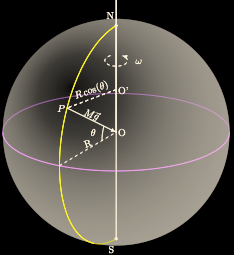
\includegraphics[width=0.6\textwidth]{Figures/Gravity/Exported/GravityFieldEarthRotation_Reversed.png}
  \end{center}
\end{PointSix}
\end{frame}




\begin{frame}
\begin{PointSix}{Gravitational field of a spherical Earth}
  \small Centripedal acceleration at P perpendicular to rotation axis parallel to O'-P:

  $$
  g_{r.} = \omega^2 R \cos(\theta)
  $$

  \small Centripedal acceleration at P perpendicular to rotation axis parallel to O'-P:

  $$
  g_{r.,proj.} = \omega^2 R \cos^2(\theta)
  $$

  \scalebox{0.6}{\parbox{\linewidth}{
    \begin{align*}
    &\text{Angular Frequency:}\, \omega \\
    &\text{Angular Velocity:}\, \vec{v}_r = \vec{\omega} \times \vec{R}\cos(\theta)\\
    &\text{Angular Acceleration:}\, \vec{g}_r = \dot{\vec{v}}_r=\vec{\omega} \times \vec{\omega} \times \vec{R}\cos(\theta)\\
    \end{align*}
  }}
\end{PointSix}
\end{frame}


\begin{frame}
\begin{PointSix}{An ellipsoidal Earth}
    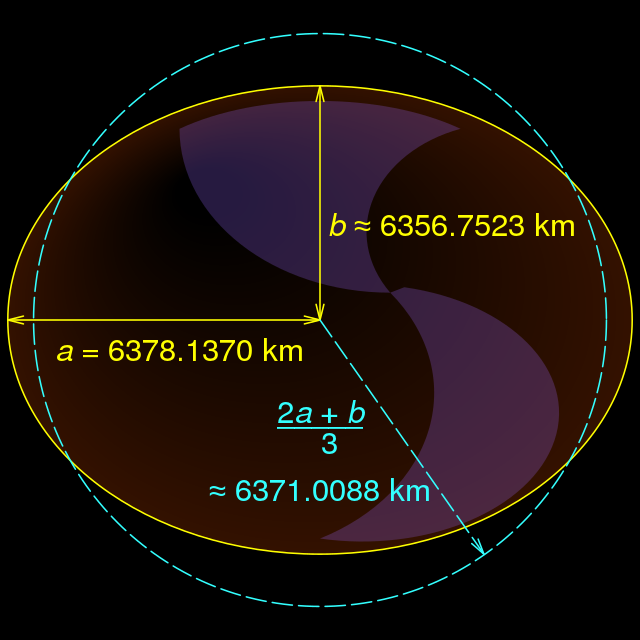
\includegraphics[width=0.8\textwidth]{Figures/Gravity/Exported/WGS84_mean_Earth_radius_Cmglee_Reversed.png}
    \tiny [Cmglee CCC 4.0]
\end{PointSix}
\end{frame}

\begin{frame}
\begin{PointSix}{Potential Fields}
  \begin{itemize}
    \item Rotation induces ellipsoidal shape approximate with reference ellipsoid.
    \item Latitudinal correction of gravitation is adjusted accordingly.
  \end{itemize}
\end{PointSix}
\end{frame}


\begin{frame}
  \begin{PointSix}{An ellipsoidal Earth}
      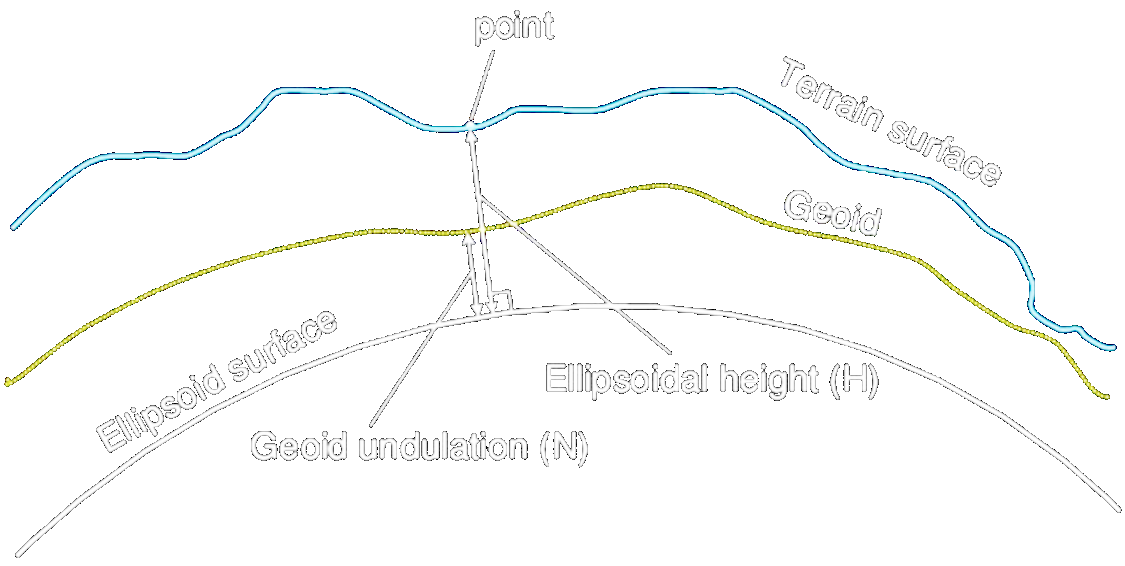
\includegraphics[width=0.9\textwidth]{Figures/Gravity/Exported/Geoid_Ziebart2004_TransparentBlack.png}

      \tiny [Ziebart et al., 2004] 

      \small
      \only<1>
      {
        \begin{itemize}
          \item Geoid is a real-world equipotential line approximating sea level.
          \item It is referenced to the geometric ellipsoid.
        \end{itemize}
      }
      \only<2>
      {
        \begin{itemize}
          \item 2 Geoid is a real-world equipotential line approximating sea level.
          \item 2 It is referenced to the geometric ellipsoid.
        \end{itemize}
      }
      \only<3>
      {
        \begin{itemize}
          \item Upwarping of geoid indicates mass excess.
          \item Downwarping of geoid indicates mass deficit.
        \end{itemize}
      }
  \end{PointSix}
  \end{frame}

%\begin{frame}
    \begin{PointSix}{Learning Goals}
      \alert{Learning goals today:}
      \begin{itemize}
        \item Principles of gravimeters.
        \item Gravity survey types (absolute \& relative) and general considerations of survey layouts and structure types.
        \item Reduction of gravity data.
      \end{itemize}
    \end{PointSix}
\end{frame}
  
\begin{frame}
    \begin{PointSix}{Spring-based gravimeters}
        \tiny [cc Reyko, CC-BY-SA3.0]
      \begin{center}
        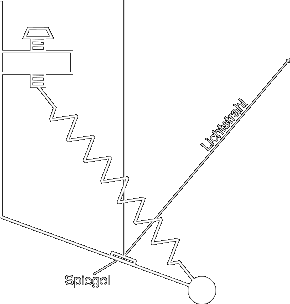
\includegraphics[width=0.6\textwidth]{Figures/Gravity/Exported/Reyko_CCBY-SA_LaCoste-Romberg_Reversed.png}
      
        \small Springconstant \& Extension.
      \end{center}
    \end{PointSix}
\end{frame}


\begin{frame}
  \begin{PointSix}{Pendulum-based gravimeters}
    
    \begin{center}
      \begin{tikzpicture}[font=\footnotesize]
        % Support
        \fill (-1.5,0) rectangle(1.5,0.1);

        % Bob's trajectory
        \draw[dashed] (-60:4) arc(-60:-120:4);

        % Rod + Bob
        \draw (0,0) -- (-60:4) node[fill,circle](m){};

        % Weight Force
        \draw[-latex] (m) -- node[right]{$\vec{g}$}++(0,-1) ;

        % Tension Force
        %\draw [-latex] (m) -- node[right]{$\vec{T}$}(-60:3);

        % Light gray pendulum
        \draw[black!10] (0,0) -- (-90:4) node[fill,circle]{};
        \draw[black!10] (0,0) -- (-120:4) node[fill,circle]{};
        \draw[<->,Karminrot] (0,0) -- (-90:4) node[midway,right]{l};
      \end{tikzpicture}

      Eigenfrequency \& Length.
      $$
      \omega = \sqrt{\frac{g}{l}}
      $$
    \end{center}
  \end{PointSix}
\end{frame}

\begin{frame}
  \begin{PointSix}{Free-fall gravimeters ($\rightarrow$ Ex.)}
      \tiny [FG Gravimeter from MicroGLaCoste]
    \begin{center}
      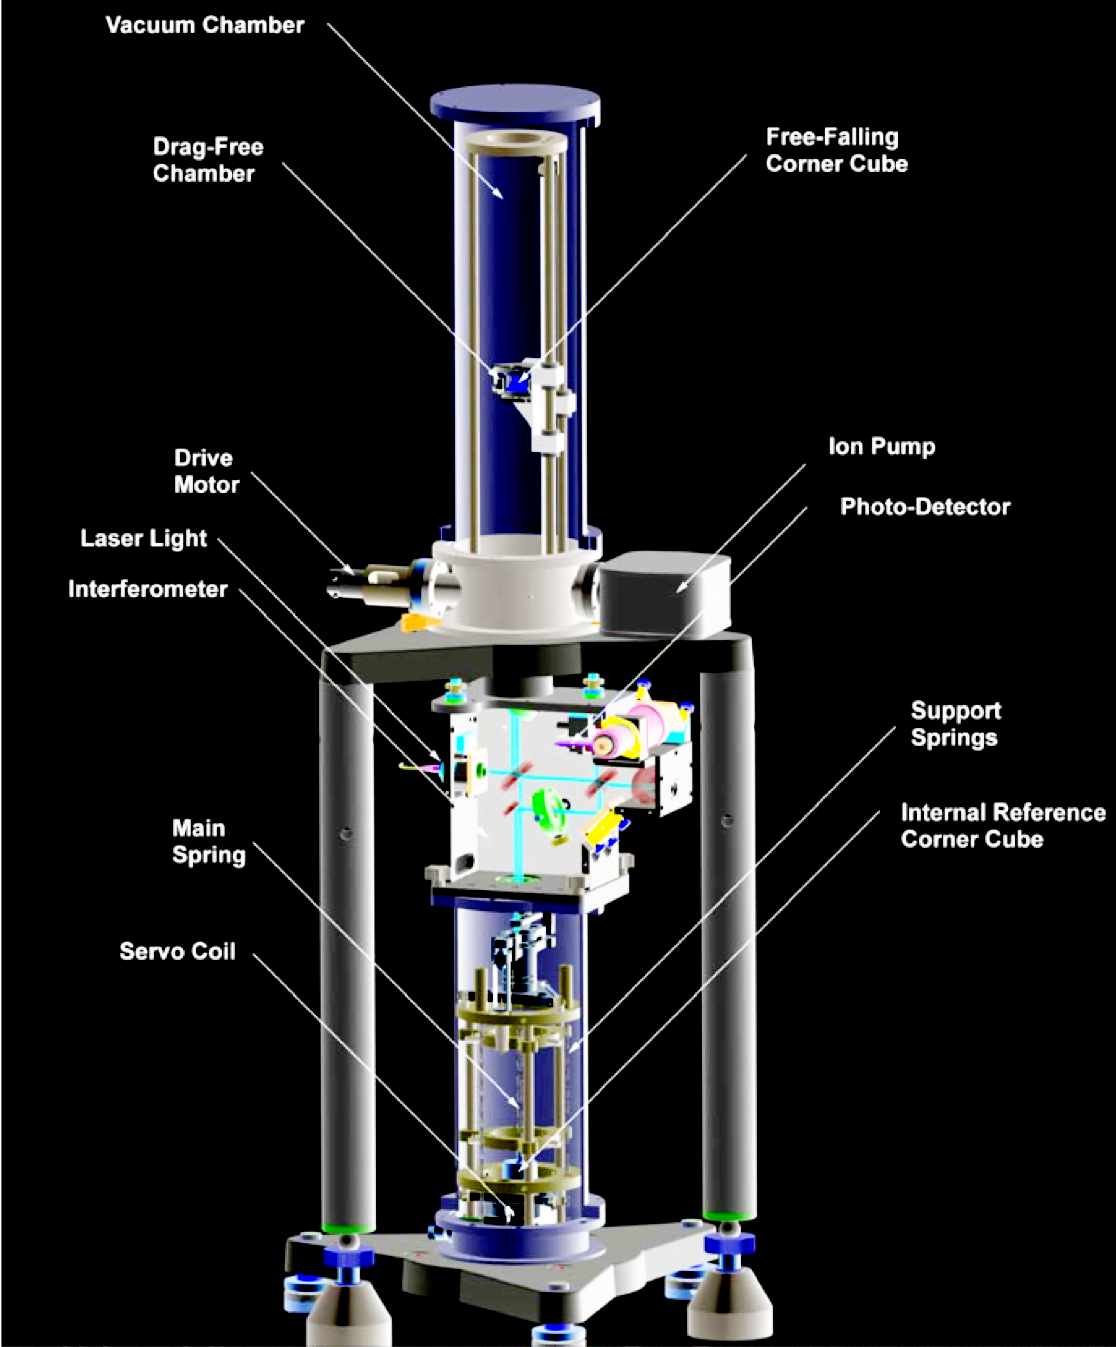
\includegraphics[width=0.55\textwidth]{Figures/Gravity/Exported/FG_Gravimeter_MicroGLaCoste_Reversed.png}

      \small Traveltime \& Distance.
    \end{center}
  \end{PointSix}
\end{frame}

\begin{frame}
  \begin{PointSix}{Gravimeters}
    \begin{itemize}
      \item Unit used is \textit{Gal} (=0.01 ms$^{-2}$)
      \item Top \textit{absolute} gravimeters $\sim 1 \mu$Gal ($10^{-9} g$)
      \item Top \textit{relative} gravimeters $\sim 10 \mu$Gal ($10^{-9} g$)
      \item Typically only $g_z$ is measured.
    \end{itemize}
  \end{PointSix}
\end{frame}
\begin{frame}
    \begin{PointSix}{Instrument drift / temporal variability}
      \resizebox{9 cm}{!}{     
              \begin{tikzpicture}[background rectangle/.style={fill=black},show background rectangle]
                \coordinate (TL) at (-2,-3);
                \coordinate (TR) at (9,-3);
                \coordinate (BL) at (-2,-10);
                \coordinate (BR) at (9,-10);
                \coordinate (Target) at (3.5,-5);

     

                \draw [->,thick,white] (TL) -- (TR) node[circle,fill=Karminrot,pos=0]{A} node[circle,fill=Karminrot,pos=0.2]{B} node[circle,fill=Karminrot,pos=0.4]{C} node[circle,fill=Karminrot,pos=0.6]{D} node[circle,fill=Karminrot,pos=0.8]{E} node[circle,fill=Karminrot,pos=1.0]{F};
                \fill[Karminrot] (Target) circle (2.5ex);
                %\draw[ultra thick,MyBlue] (-1.4,1.3) circle (2.5ex);
                %\draw [<-,line width=1.25mm,MyBlue]  (TL) to[out=30,in=150] (TR);
                \begin{axis}[
                    ylabel={Gravity Anomaly},
                    xlabel={Horizontal Distance},
                    label style={font=\small},
                    axis lines=middle, xtick=\empty,ytick=\empty,
                    color=white,
                    width=12cm,
                    height=\axisdefaultheight,
                    at={(-0.18\linewidth,0)},
                    axis line style=ultra thick,
                    x label style={at={(axis description cs:0.91,-0.025)},anchor=north},
                    y label style={at={(axis description cs:0.91,0.9)},anchor=north}
                      ]
                    \addplot[domain=-80:80,samples=200,color=Karminrot,line width=1.0mm] {5/((25+x*x)^(0.5)*1000)+x/1000000+1/10000};
                    %\addplot[domain=-80:80,samples=200,color=MyBlue,line width=1.0mm,dashed] {5/((25+x*x)^(0.5)*1000)};
                    %\addplot[domain=-80:-70,samples=200,color=Karminrot,mark=-*,line width=1.0mm,dashed] {x*0.0+3/10000};
                  \end{axis}
              \end{tikzpicture}
      }
    \end{PointSix}
\end{frame}


\begin{frame}
  \begin{PointSix}{Instrument drift / temporal variability}
    \resizebox{9 cm}{!}{     
            \begin{tikzpicture}[background rectangle/.style={fill=black},show background rectangle]
              \coordinate (TL) at (-2,-3);
              \coordinate (TR) at (9,-3);
              \coordinate (BL) at (-2,-10);
              \coordinate (BR) at (9,-10);
              \coordinate (Target) at (3.5,-5);

   

              \draw [->,thick,white] (TL) -- (TR) node[circle,fill=Karminrot,pos=0]{A} node[circle,fill=Karminrot,pos=0.2]{B} node[circle,fill=Karminrot,pos=0.4]{C} node[circle,fill=Karminrot,pos=0.6]{D} node[circle,fill=Karminrot,pos=0.8]{E} node[circle,fill=Karminrot,pos=1.0]{F};
              \fill[Karminrot] (Target) circle (2.5ex);
              \draw[ultra thick,MyBlue] (-1.4,1.3) circle (2.5ex);
              \node[MyBlue] at (-1.4,2.4) {offset};
              \draw [<-,line width=1.25mm,MyBlue]  (TL) to[out=30,in=150] (TR);
              \begin{axis}[
                  ylabel={Gravity Anomaly},
                  xlabel={Horizontal Distance},
                  label style={font=\small},
                  axis lines=middle, xtick=\empty,ytick=\empty,
                  color=white,
                  width=12cm,
                  height=\axisdefaultheight,
                  at={(-0.18\linewidth,0)},
                  axis line style=ultra thick,
                  x label style={at={(axis description cs:0.91,-0.025)},anchor=north},
                  y label style={at={(axis description cs:0.91,0.9)},anchor=north}
                    ]
                  \addplot[domain=-80:80,samples=200,color=Karminrot,line width=1.0mm] {5/((25+x*x)^(0.5)*1000)+x/1000000+1/10000};
                  \addplot[domain=-80:80,samples=200,color=MyBlue,line width=1.0mm,dashed] {5/((25+x*x)^(0.5)*1000)};
                  \addplot[domain=-80:-70,samples=200,color=Karminrot,mark=-*,line width=1.0mm,dashed] {x*0.0+3/10000};
                \end{axis}
            \end{tikzpicture}
    }
  \end{PointSix}
\end{frame}

\begin{frame}
  \begin{PointSix}{Absolute vs. relative}
    Absolute gravimeters are needed
    \begin{itemize}
      \item if loop closure if impossible (e.g. intercontinental surveys),
      \item for long-term changes such as isostatic uplift,
      \item as basestations for relative surveys.
    \end{itemize}
    Relative surveys are always easier to conduct and loop closure can cancel many error sources (e.g., instrument drift).
  \end{PointSix}
\end{frame}

\begin{frame}
  \begin{PointSix}{Reduction of gravity data}
    Every gravity survey measures:
    \begin{itemize}
      \item latitudinal variability,
      \item dependency on elevation,
      \item the surrounding terrain,
      \item excess mass above anomaly,
      \item earth \& ocean tides,
      \item (instr. drift, motion compons.).
      \item \alert{density variability in the subsurface.}
    \end{itemize}
  \end{PointSix}
\end{frame}

\begin{frame}
  \begin{PointSix}{Latitudinal variability ($\rightarrow$ Ex.)}
    \small  Extension to ellipsoid contains the same physics.
    \begin{center}
    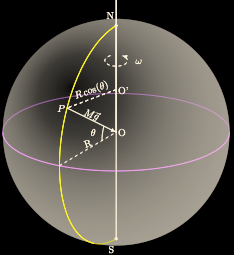
\includegraphics[width=0.5\textwidth]{Figures/Gravity/Exported/GravityFieldEarthRotation_Reversed.png}
    \end{center}
    \small Max 5 Gal (this is large!).
  \end{PointSix}
\end{frame}

\begin{frame}
  \begin{PointSix}{Reduction of gravity data}
    Every gravity survey measures:
    \begin{itemize}
      \item \textcolor{MyBlue}{latitudinal variability},
      \item dependency on elevation,
      \item the surrounding terrain,
      \item excess mass above anomaly,
      \item earth \& ocean tides,
      \item (instr. drift, motion compons.).
      \item \alert{density variability in the subsurface.}
    \end{itemize}
  \end{PointSix}
\end{frame}

\begin{frame}
  \begin{PointSix}{Elevation correction (i.e. free-air)}
    \resizebox{9 cm}{!}{     
            \begin{tikzpicture}[background rectangle/.style={fill=black},show background rectangle]
              \coordinate (TL) at (-2,-3);
              \coordinate (TR) at (9,-3);
              \coordinate (BL) at (-2,-10);
              \coordinate (BR) at (9,-10);
              \coordinate (Target) at (3.5,-5);

   

              \draw [->,thick,white] (TL) -- (TR) node[circle,fill=Karminrot,pos=0]{A} node[circle,fill=Karminrot,pos=0.2]{B} node[circle,fill=Karminrot,pos=0.4]{C} node[circle,fill=Karminrot,pos=0.6]{D} node[circle,fill=Karminrot,pos=0.8]{E} node[circle,fill=Karminrot,pos=1.0]{F};
              \fill[Karminrot] (Target) circle (2.5ex);
              \begin{axis}[
                  ylabel={Gravity Anomaly},
                  xlabel={Horizontal Distance},
                  label style={font=\small},
                  axis lines=middle, xtick=\empty,ytick=\empty,
                  color=white,
                  width=12cm,
                  height=\axisdefaultheight,
                  at={(-0.18\linewidth,0)},
                  axis line style=ultra thick,
                  x label style={at={(axis description cs:0.91,-0.025)},anchor=north},
                  y label style={at={(axis description cs:0.91,0.9)},anchor=north}
                    ]
                 % \addplot[domain=-80:80,samples=200,color=Karminrot,line width=1.0mm] {5/((25+x*x)^(0.5)*1000)+x/1000000+1/10000};
                  \addplot[domain=-80:80,samples=200,color=MyBlue,line width=1.0mm] {5/((25+x*x)^(0.5)*1000)};
                  %\addplot[domain=-80:-70,samples=200,color=Karminrot,mark=-*,line width=1.0mm,dashed] {x*0.0+3/10000};
                \end{axis}
            \end{tikzpicture}
    }
  \end{PointSix}
\end{frame}

\begin{frame}
  \begin{PointSix}{Elevation correction (i.e. free-air)}
    \resizebox{9 cm}{!}{     
            \begin{tikzpicture}[background rectangle/.style={fill=black},show background rectangle]
              \coordinate (TL) at (-2,-2);
              \coordinate (TR) at (9,-2);
              \coordinate (BL) at (-2,-10);
              \coordinate (BR) at (9,-10);
              \coordinate (Target) at (3.5,-5);

   

              \draw [->,thick,white] (TL) -- (TR) node[circle,fill=Karminrot,pos=0]{A} node[circle,fill=Karminrot,pos=0.2]{B} node[circle,fill=Karminrot,pos=0.4]{C} node[circle,fill=Karminrot,pos=0.6]{D} node[circle,fill=Karminrot,pos=0.8]{E} node[circle,fill=Karminrot,pos=1.0]{F};
              \fill[Karminrot] (Target) circle (2.5ex);
              \begin{axis}[
                  ylabel={Gravity Anomaly},
                  xlabel={Horizontal Distance},
                  label style={font=\small},
                  axis lines=middle, xtick=\empty,ytick=\empty,
                  color=white,
                  width=12cm,
                  height=\axisdefaultheight,
                  at={(-0.18\linewidth,0)},
                  axis line style=ultra thick,
                  x label style={at={(axis description cs:0.91,-0.025)},anchor=north},
                  y label style={at={(axis description cs:0.91,0.9)},anchor=north}
                    ]
                 % \addplot[domain=-80:80,samples=200,color=Karminrot,line width=1.0mm] {5/((25+x*x)^(0.5)*1000)+x/1000000+1/10000};
                 \addplot[domain=-80:80,samples=200,color=MyBlue,line width=1.0mm,dashed] {5/((25+x*x)^(0.5)*1000)};
                  \addplot[domain=-80:80,samples=200,color=MyBlue,line width=1.0mm] {0.6*5/((25+x*x)^(0.5)*1000)};
                  %\addplot[domain=-80:-70,samples=200,color=Karminrot,mark=-*,line width=1.0mm,dashed] {x*0.0+3/10000};
                \end{axis}
            \end{tikzpicture}
    }
  \end{PointSix}
\end{frame}

\begin{frame}
  \begin{PointSix}{Elevation correction}
    The elevation correction references the gravity anomaly to the same datum (e.g., the geoid). 
    
    \alert{How does the gravitational acceleration change with elevation near the Earth's surface?}
  \end{PointSix}
\end{frame}

\begin{frame}
  \begin{PointSix}{Elevation correction via Taylor expansion}
    Taylor expansion near $r=R_E$:
    \only<1>
    {
      $$
        g(r) = g(R_E) + \frac{dg}{dr}|_{R_E}
      $$
    }
    \only<2>
    {
      $$
        g(r) \approx G\frac{M}{R_E^2} - 2G\frac{M}{R_E^3}(r-R_E) + ...
      $$
    }
    \only<3>
    {
      $$
        g(r) \approx \underbrace{G\frac{M}{R_E^2}}_{\text{g at Earth's surface}} - 2G\frac{M}{R_E^3}(r-R_E) + ...
      $$
    }
    \only<4>
    {
      $$
        g(r) \approx G\frac{M}{R_E^2} - \underbrace{2G\frac{M}{R_E^3}(r-R_E)}_{\text{change with elevation}} + ...
      $$
    }
    \only<5>
    {
      $$
        g(r) \approx G\frac{M}{R_E^2} - \underbrace{2G\frac{M}{R_E^3}(r-R_E)}_{\text{change with elevation}} + ...
      $$
      Evaluation at let's say $r=R_E+1$ (m) returns a change of $\delta g(r)\approx -0.3$ mGal per m.
    }
    \only<6>
    {
      $$
        g(r) \approx G\frac{M}{R_E^2} - \underbrace{2G\frac{M}{R_E^3}(r-R_E)}_{\text{change with elevation}} + ...
      $$
      $\delta g(r)\approx -0.3$ mGal per m is large compared to the sensitivity of gravimeters, \alert{therefore the gravimeter elevation needs to be determined within centimeters using GNSS.}
    }
  \end{PointSix}
\end{frame}

\begin{frame}
  \begin{PointSix}{Reduction of gravity data}
    Every gravity survey measures:
    \begin{itemize}
      \item \textcolor{MyBlue}{latitudinal variability},
      \item \textcolor{MyBlue}{dependency on elevation},
      \item the surrounding terrain,
      \item excess mass above anomaly,
      \item earth \& ocean tides,
      \item (instr. drift, motion compons.).
      \item \alert{density variability in the subsurface.}
    \end{itemize}
  \end{PointSix}
\end{frame}

\begin{frame}
  \begin{PointSix}{Reduction of gravity data: Terrain correction}
   \begin{tikzpicture}
      \coordinate (TL) at (-2,-2);
      \coordinate (TR) at (9,-2);
      \coordinate (BL) at (-2,-10);
      \coordinate (BR) at (9,-10);
      \coordinate (Target) at (3.5,-3);

      \draw [->,thick,white] ([xshift=4cm,yshift=2cm] TL) -- ([yshift=2cm] TR);
      %\draw [->,thick,white,dashed] (TL) -- (TR) node[draw=none,fill=none,font=\scriptsize,near start,below] {reference surface};
      %\draw ([yshift=2cm] TL) .. controls ([xshift=2cm,yshift=4cm] TL) .. ([xshift=4.0cm,yshift=2cm] TL) ;
      \draw ([yshift=2cm] TL) ([xshift=4.0cm,yshift=2cm] TL) ;
      \fill[Karminrot] (Target) circle (2.5ex);
      %\draw [->, line width=1.5mm](3.5,0) -- (2.7,-1.7);
      \draw [->, line width=1.5mm,dashed](3.5,0) -- (3.5,-2);
     %\draw [line width=1.0mm,dashed](2.7,-1.7) -- (0,1) node[draw=none,fill=none,font=\small,midway,below,rotate=-46] {mass excess};
   \end{tikzpicture}
  \end{PointSix}
\end{frame}


\begin{frame}
  \begin{PointSix}{Reduction of gravity data: Terrain correction}
   \begin{tikzpicture}
      \coordinate (TL) at (-2,-2);
      \coordinate (TR) at (9,-2);
      \coordinate (BL) at (-2,-10);
      \coordinate (BR) at (9,-10);
      \coordinate (Target) at (3.5,-3);

      \draw [->,thick,white] ([xshift=4cm,yshift=2cm] TL) -- ([yshift=2cm] TR);
      %\draw [->,thick,white,dashed] (TL) -- (TR) node[draw=none,fill=none,font=\scriptsize,near start,below] {reference surface};
      \draw ([yshift=2cm] TL) .. controls ([xshift=2cm,yshift=4cm] TL) .. ([xshift=4.0cm,yshift=2cm] TL) ;
      \fill[Karminrot] (Target) circle (2.5ex);
      \draw [->, line width=1.5mm](3.5,0) -- (2.7,-2);
      \draw [->, line width=1.5mm,dashed](3.5,0) -- (3.5,-2);
      \draw [line width=1.0mm,dashed](2.7,-2) -- (0,1) node[draw=none,fill=none,font=\small,midway,below,rotate=-46] {mass excess};
   \end{tikzpicture}
  A neighboring mountain will reduce the measured $g_z$ independent of target properties.
  \end{PointSix}
\end{frame}
\begin{frame}
  \begin{PointSix}{Reduction of gravity data: Terrain correction}
   \begin{tikzpicture}
      \coordinate (TL) at (-2,-2);
      \coordinate (TR) at (9,-2);
      \coordinate (BL) at (-2,-10);
      \coordinate (BR) at (9,-10);
      \coordinate (Target) at (3.5,-3);

      \draw [->,thick,white] ([xshift=4cm,yshift=2cm] TL) -- ([yshift=2cm] TR);
      %\draw [->,thick,white,dashed] (TL) -- (TR) node[draw=none,fill=none,font=\scriptsize,near start,below] {reference surface};
      \draw ([yshift=2cm] TL) .. controls ([xshift=2cm,yshift=0cm] TL) .. ([xshift=4.0cm,yshift=2cm] TL) ;
      \fill[Karminrot] (Target) circle (2.5ex);
      \draw [->, line width=1.5mm](3.5,0) -- (4.3,-2);
      \draw [->, line width=1.5mm,dashed](3.5,0) -- (3.5,-2);
      \draw [line width=1.0mm,dashed](3.5,-2) -- (0,-1) node[draw=none,fill=none,font=\small,midway,below,rotate=-20] {mass deficit};
   \end{tikzpicture}
  A neighboring valley will reduce the measured $g_z$ independent of target properties.
  \end{PointSix}
\end{frame}

\begin{frame}
  \begin{PointSix}{Reduction of gravity data: Terrain correction}
  \begin{itemize}
    \item The terrain correction requires an elevation model and assumptions about the broad-scale sub-surface density.
    \item The terrain correction is positive both for surrounding valleys and mountains.
  \end{itemize}
\end{PointSix}
\end{frame}

\begin{frame}
  \begin{PointSix}{Reduction of gravity data}
    Every gravity survey measures:
    \begin{itemize}
      \item \textcolor{MyBlue}{latitudinal variability},
      \item \textcolor{MyBlue}{dependency on elevation},
      \item \textcolor{MyBlue}{the surrounding terrain},
      \item excess mass above anomaly,
      \item earth \& ocean tides,
      \item (instr. drift, motion compons.).
      \item \alert{density variability in the subsurface.}
    \end{itemize}
  \end{PointSix}
\end{frame}

\begin{frame}
  \begin{PointSix}{Reduction of gravity data: Terrain correction}
   \begin{tikzpicture}
      \coordinate (TL) at (-2,-2);
      \coordinate (TR) at (9,-2);
      \coordinate (BL) at (-2,-10);
      \coordinate (BR) at (9,-10);
      \coordinate (Target) at (3.5,-3);

      \draw [->,thick,white] ([xshift=4cm,yshift=2cm] TL) -- ([yshift=2cm] TR);
      \draw [->,thick,white,dashed] (TL) -- (TR) node[draw=none,fill=none,font=\scriptsize,near start,below] {reference surface};
      \draw ([yshift=2cm] TL) .. controls ([xshift=2cm,yshift=4cm] TL) .. ([xshift=4.0cm,yshift=2cm] TL) ;
      \fill[Karminrot] (Target) circle (2.5ex);
      \draw [->, line width=1.5mm,Karminrot](3.5,0) -- (3.5,-1);

   \end{tikzpicture}
  \small Elevation and terrain correction to not account for the mass between the measurement surface and the reference surface.
  \end{PointSix}
\end{frame}

\begin{frame}
  \begin{PointSix}{Reduction of gravity data: Terrain correction}
   \begin{tikzpicture}
      \coordinate (TL) at (-2,-2);
      \coordinate (TR) at (9,-2);
      \coordinate (BL) at (-2,-10);
      \coordinate (BR) at (9,-10);
      \coordinate (Target) at (3.5,-3);

      %\draw [->,thick,white] ([xshift=4cm,yshift=2cm] TL) -- ([yshift=2cm] TR);
      %\draw [->,thick,green,name path = A] ([yshift=2cm] TL) -- ([yshift=2cm] TR);
      \draw [->,thick,white,dashed,name path = B] (TL) -- (TR) node[draw=none,fill=none,font=\scriptsize,near start,below] {reference surface};
      \draw ([yshift=2cm] TL) .. controls ([xshift=2cm,yshift=4cm] TL) .. ([xshift=4.0cm,yshift=2cm] TL) ;
      \fill[Karminrot] (Target) circle (2.5ex);
      \fill[pattern=north west lines,pattern color=white] ([yshift=2cm] TL) rectangle (TR);
      \draw [->, line width=1.5mm,Karminrot](3.5,0) -- (3.5,-1);
      \draw [|-|, line width=0.5mm,white]([xshift=-0.5cm] TL) -- ([xshift=-0.5cm, yshift=2cm] TL) node[draw=none,fill=none,font=\scriptsize,midway,left] {h};;
      
   \end{tikzpicture}
  \only<1>{
    \small What is the effect $\delta g_z$ of a horizontal plate with constant density?
  }
  \only<2>{
    \small $g_z = G \rho \int \int \int \frac{1}{r^2}\cos(\phi) dV = ? $
  }
  \only<3>{
    \small $g_z = G \rho \int \int \int \frac{1}{r^2}\cos(\phi) dV = 2\pi G\rho h$
  }
  \end{PointSix}
\end{frame}
\begin{frame}
  \begin{PointSix}{Reduction of gravity data}
    Every gravity survey measures:
    \begin{itemize}
      \item \textcolor{MyBlue}{latitudinal variability},
      \item \textcolor{MyBlue}{dependency on elevation},
      \item \textcolor{MyBlue}{the surrounding terrain},
      \item \textcolor{MyBlue}{excess mass above anomaly},
      \item earth \& ocean tides,
      \item (instr. drift, motion compensation),
      \item \alert{density variability in the subsurface.}
    \end{itemize}
  \end{PointSix}
\end{frame}

\begin{frame}
  \begin{PointSix}{The origin of tides}
      \begin{itemize}
        \item Tides are caused by gravity celestial bodies (i.e. Sun \& Moon).
        \item Tidal forces vary across a spatially extended body.
        \item Tidal forces are balanced by centrifugal forces of two (three) body rotations.
      \end{itemize}
  \end{PointSix}
\end{frame}

\begin{frame}
  \begin{PointSix}{The origin of tides}
  \begin{tikzpicture}
    \coordinate (EC) at (5,0) node[yshift=-2cm,draw=none,fill=none,font=\small,below] {Earth};
    \coordinate (MC) at (0,0) node[yshift=-2cm,xshift=5cm,draw=none,fill=none,font=\small,below] {Moon};
    \fill[white] (EC) circle (4.5ex);
    \fill[white] (MC) circle (1.5ex);
    %§\draw [->, line width=1.5mm,Karminrot](EC) -- (MC);
    % \begin{axis}[
    %   ylabel={F},
    %   xlabel={distance r},
    %   label style={font=\tiny},
    %   axis lines=middle, xtick=\empty,ytick=\empty,
    %   color=Karminrot,
    %   width=8cm,
    %   height=4cm,
    %   ymin=0.0,
    %   %ymax=5.16,
    %   at={(0.0\linewidth,0.0\linewidth)},
    %   axis line style=ultra thick,
    %   x label style={at={(axis description cs:0.4,-0.025)},anchor=north},
    %   y label style={at={(axis description cs:-0.1,0.9)},anchor=north}
    %     ]

    %  \addplot[domain=0.6:1.5,samples=200,color=MyBlue,line width=1.0mm,dashed] {1/(x*x))};
    % \end{axis}
  \end{tikzpicture}
  \end{PointSix}
\end{frame}

\begin{frame}
  \begin{PointSix}{The origin of tides}
  \begin{tikzpicture}
    \coordinate (EC) at (5,0) node[yshift=-2cm,draw=none,fill=none,font=\small,below] {Moon};
    \coordinate (MC) at (0,0) node[yshift=-2cm,xshift=5cm,draw=none,fill=none,font=\small,below] {Earth};
    \fill[white] (EC) circle (4.5ex);
    \fill[white] (MC) circle (1.5ex);
    %§\draw [->, line width=1.5mm,Karminrot](EC) -- (MC);
    \begin{axis}[
      ylabel={F},
      xlabel={distance r},
      label style={font=\tiny},
      axis lines=middle, xtick=\empty,ytick=\empty,
      color=Karminrot,
      width=8cm,
      height=4cm,
      ymin=0.0,
      %ymax=5.16,
      at={(0.0\linewidth,0.0\linewidth)},
      axis line style=ultra thick,
      x label style={at={(axis description cs:0.4,-0.025)},anchor=north},
      y label style={at={(axis description cs:-0.1,0.9)},anchor=north}
        ]

     \addplot[domain=0.6:1.5,samples=200,color=MyBlue,line width=1.0mm,dashed] {1/(x*x))};
    \end{axis}
  \end{tikzpicture}
  \vspace{1cm}

  \small Gravitational attraction is stronger on the nearside than the farside.
  \end{PointSix}
\end{frame}

\begin{frame}
  \begin{PointSix}{The origin of tides}
    \begin{tikzpicture}
        \coordinate (EC) at (5,0);
        \coordinate (MC) at (0,0);
        \coordinate (RP) at (4,0);
        \fill[white] (EC) circle (4.5ex) node[yshift=-2cm,draw=none,fill=none,font=\small,below] {Earth};
        \fill[white] (MC) circle (1.5ex) node[yshift=-2cm,draw=none,fill=none,font=\small,below] {Moon};
        \fill[Karminrot] (RP) circle (0.5ex);
        \draw [->,thick,Karminrot] (RP) -- ([yshift=2cm] RP) node [midway] {\AxisRotator[rotate=-90]};
        \draw [|-|,thick,Karminrot] (EC) -- (MC);
   \end{tikzpicture}
   
          \pause
          \small Centrifugal force can be projected into radial (i.e. parallel to Earth's gravitation) and parallel component. This leads to the force balance.
  \end{PointSix}
\end{frame}

\begin{frame}
  \begin{PointSix}{The origin of tides}
  \begin{tikzpicture}
    \coordinate (RP) at (1,0);
    \node[inner sep=0pt] (russell) at (0,0)
      {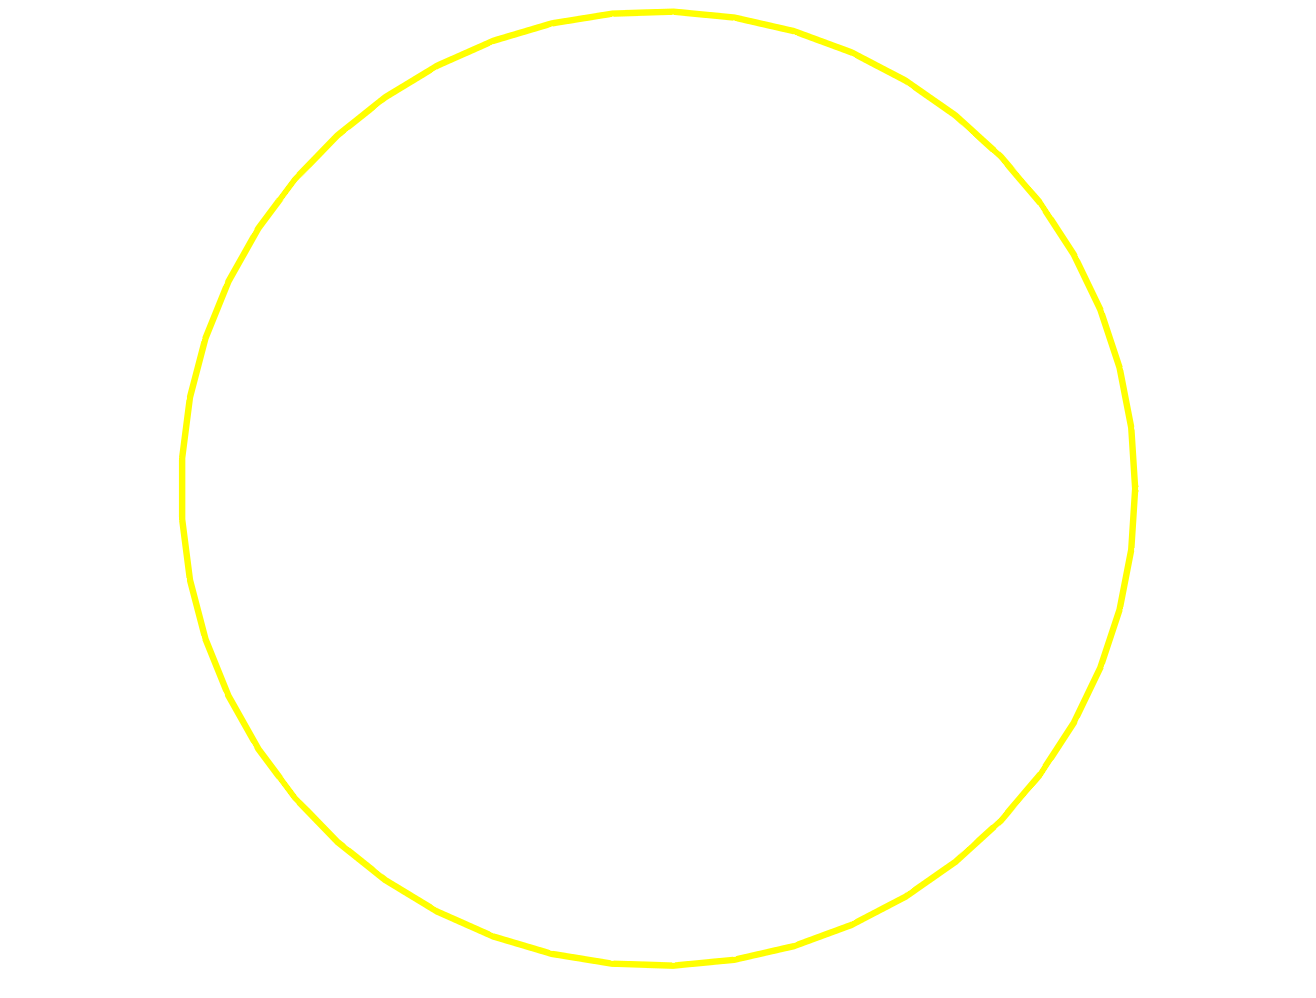
\includegraphics[width=.6\textwidth]{Figures/Gravity/Exported/Field_tidal.png}};
      \fill[white] (5,0) circle (1.5ex) node[yshift=-2cm,draw=none,fill=none,font=\small,below] {Moon};
      \draw [->,thick,Karminrot] (RP) -- ([yshift=2cm] RP) node [midway] {\AxisRotator[rotate=-90]};
      \draw [|-|,thick,Karminrot] (RP) -- (5,0);
  \end{tikzpicture}
  \small The lunar gravity differential field is responsible for two tidal bulges (i.e. tides twice a day).
\end{PointSix}
\end{frame}

\begin{frame}
  \begin{PointSix}{The origin of tides}
      \small
      \begin{itemize}
        \item Tidal forces vary across a spatially extended body.
        \item Tidal forces are balanced by centrifugal forces of two (three) body rotations.
        \item There is lots of confusion regarding the origin of tides (cf. Matsuda et al. 2015 $\rightarrow$ Ilias).
        \item \color{MyBlue}{Tide models can be used for correction} 
      \end{itemize}
  \end{PointSix}
\end{frame}

\begin{frame}
  \begin{PointSix}{Reduction of gravity data}
    Every gravity survey measures:
    \begin{itemize}
      \item \textcolor{MyBlue}{latitudinal variability},
      \item \textcolor{MyBlue}{dependency on elevation},
      \item \textcolor{MyBlue}{the surrounding terrain},
      \item \textcolor{MyBlue}{excess mass above anomaly},
      \item \textcolor{MyBlue}{earth \& ocean tides},
      \item (instr. drift, motion compensation),
      \item \alert{density variability in the subsurface.}
    \end{itemize}
  \end{PointSix}
\end{frame}

\begin{frame}
  \begin{PointSix}{Reduction of gravity data}
    Every gravity survey measures:
    \begin{itemize}
      \item \textcolor{MyBlue}{latitudinal variability},
      \item \textcolor{MyBlue}{dependency on elevation},
      \item \textcolor{MyBlue}{the surrounding terrain},
      \item \textcolor{MyBlue}{excess mass above anomaly},
      \item \textcolor{MyBlue}{earth \& ocean tides},
      \item \textcolor{MyBlue}{(instr. drift, motion compensation)},
      \item \alert{density variability in the subsurface.}
    \end{itemize}
  \end{PointSix}
\end{frame}
%\begin{frame}
    \begin{PointSix}{Learning Goals}
      \alert{Learning goals today:}
      \begin{itemize}
        \item Peak into applications
        \item Principals about magnetic fields (i.e., dipole field, $\vec{H}$,$\vec{B}$,$\vec{M}$,$\chi$)
        \item The Earth's magnetic field (T,H,D,I,..)
        \item The idea behind magnetic surveys.
      \end{itemize}
    \end{PointSix}
\end{frame}



\begin{frame}
  \begin{PointSix}{Example Applications}
    
    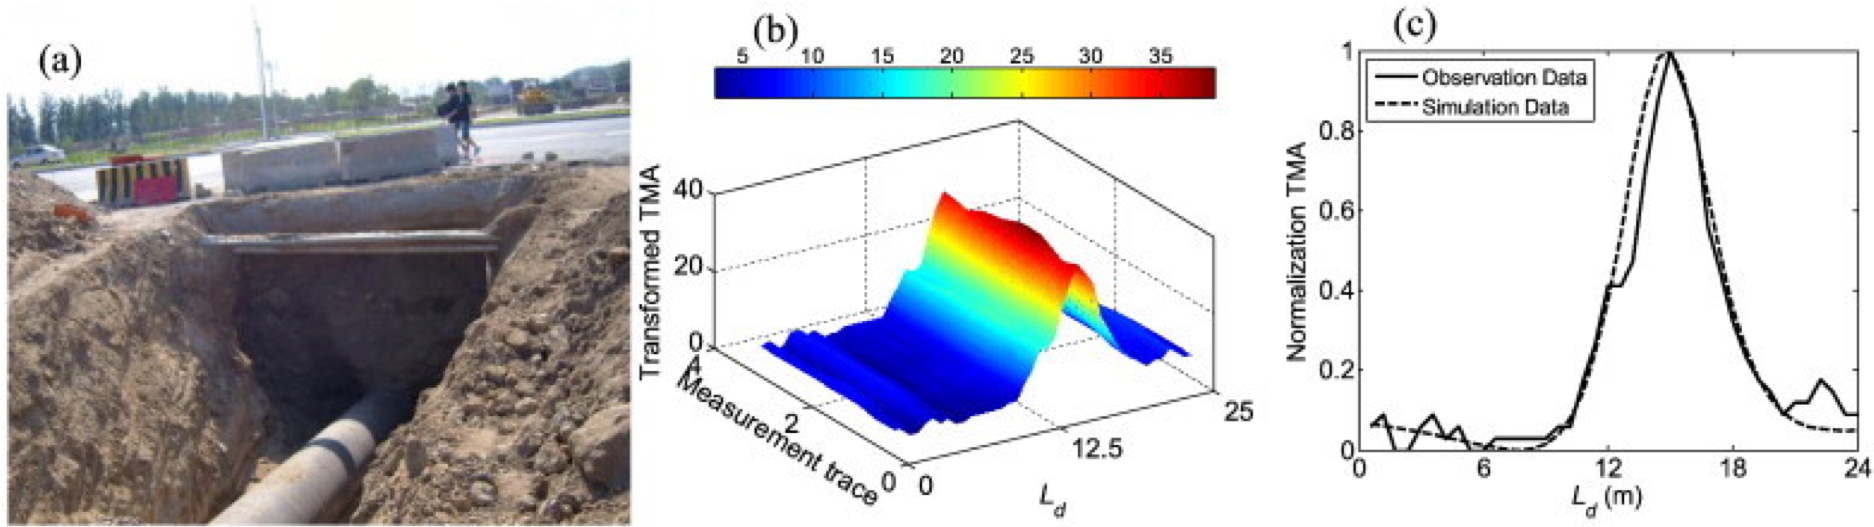
\includegraphics[width=\linewidth]{Figures/Magnetics/Pipeline_Guoetal2014_JApplPhysics.png}
  
    \tiny [Guo et al., 2014, J. Appl. Geophys.]
  \end{PointSix}
\end{frame}

\begin{frame}
  \begin{PointSix}{Example Applications}
    
    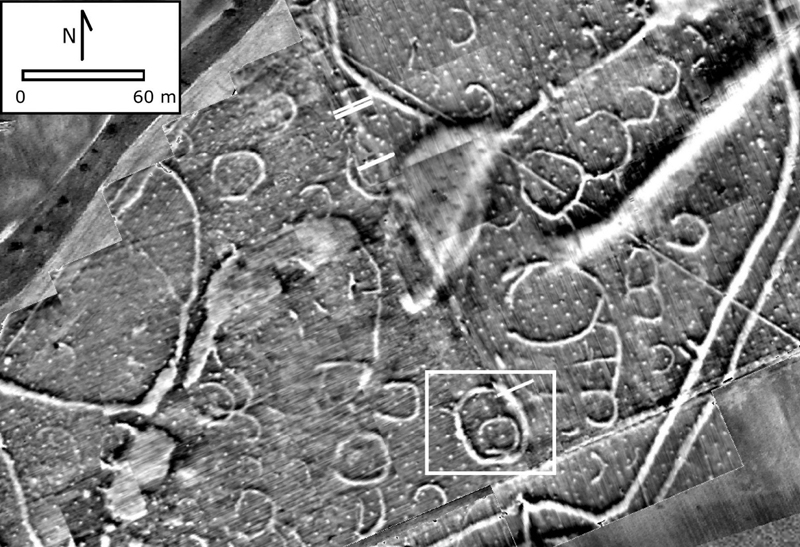
\includegraphics[width=\linewidth]{Figures/Magnetics/Archeology_CiminaleEtAl_2009_ArcheoSciences.jpg}
    %Dipole field removed. Information mirrors mostly crustal rock composition.
    \tiny [Ciminale et al., 2009, Archeosciences.]
  \end{PointSix}
\end{frame}

\begin{frame}
  \begin{PointSix}{Example Applications}
    
    \includegraphics[width=\linewidth]{Figures/Magnetics/GlobalAnomalyMap_KorhonenEtAl_2007_CommissionGeologicalMapOfTheWorld.pdf}
    %Dipole field removed. Information mirrors mostly crustal rock composition.
    \tiny [Korhonen et al., 2007, C. Geolog. Map., Paris, France.]
  \end{PointSix}
\end{frame}

\begin{frame}
  \begin{PointSix}{Fundamentals}
    What causes a magnetic field? 
  \end{PointSix}
\end{frame}

\begin{frame}
  \begin{PointSix}{Fundamentals}
    What causes a magnetic field?
    \begin{itemize}
      \item Let's use an analog to the point mass in the gravity method
      \item Let's represent 'north' and 'south' poles with point charges
      \item Let's derive the potential $A$ of a pair of positive-negative point masses
      \item Let's get the field using $\vec{B} = \nabla A$
    \end{itemize} 
  \end{PointSix}
\end{frame}

\begin{frame}
  \begin{PointSix}{The magnetic dipole potential}
    %http://hyperphysics.phy-astr.gsu.edu/hbase/electric/dipole.html
    \begin{tikzpicture}
    
      \coordinate (Qm) at ( 0,0);
      \coordinate (Qp) at (5,0);
      \coordinate (Center) at (2.5,0);
      \coordinate (P) at (4,4);
      \draw[o-o,thick] (Qm) -- (Qp) node[midway, below] {$2l$};
      \draw[-o,thick] (Center) -- (P) node[midway, left] {$r$};
      \draw[-,thick] (Qm) -- (P) node[midway, left] {$r_1$};
      \draw[-,thick] (Qp) -- (P) node[midway, right] {$r_2$};
      \node at (Qm) [below = 1mm of Qm] {$'+'$};
      \node at (Qm) [below = 10mm of Qm] {\Large $\frac{p}{r
      _1}$};
      \node at (Qp) [below = 10mm of Qp] {\Large $-\frac{p}{r
      _2}$};
      \node at (Qp) [below = 1mm of Qp] {$'-'$};
      \node at (P) [right = 1mm of P] {$P$};
      \pic [draw, ->, "$\theta$", angle eccentricity=1.5] {angle = Qp--Center--P};
    \end{tikzpicture}

  \small Use 'magnetic' potential in analogy to gravity potential
  \end{PointSix}
\end{frame}

\begin{frame}
  %http://hyperphysics.phy-astr.gsu.edu/hbase/electric/dipole.html
  \begin{PointSix}{The magnetic dipole potential}
    \begin{align*}
      A & =  \frac{p}{r_1} - \frac{p}{r_2} \\
        & =  \frac{p(r_2-r_1)}{r_1r_2}
    \end{align*}
  \end{PointSix}
\end{frame}



\begin{frame}
  %http://hyperphysics.phy-astr.gsu.edu/hbase/electric/dipole.html
  \begin{PointSix}{The magnetic dipole potential: farfield}
    \begin{tikzpicture}
    
      \coordinate (Qm) at ( 0,0);
      \coordinate (Qp) at (3,0);
      \coordinate (Center) at (1.5,0);
      \coordinate (P) at (8,4);
      \draw[o-o,thick] (Qm) -- (Qp) node[midway, below] {$2l$};
      \draw[-o,thick] (Center) -- (P) node[midway, left] {$r$};
      \draw[-,thick] (Qm) -- (P) node[midway, left] {$r_1$};
      \draw[-,thick] (Qp) -- (P) node[midway, right] {$r_2$};
      \node at (Qm) [below = 1mm of Qm] {$'+'$};
      \node at (Qp) [below = 1mm of Qp] {$'-'$};
      \node at (P) [right = 1mm of P] {$P$};
      \pic [draw, ->, "$\theta$", angle eccentricity=1.5] {angle = Qp--Center--P};
    \end{tikzpicture}
    \begin{align*}
      A & =  \frac{p(r_2-r_1)}{r_1r_2} \qquad \text{for} \qquad r \gg l
    \end{align*}
     \end{PointSix}
\end{frame}

\begin{frame}
  %http://hyperphysics.phy-astr.gsu.edu/hbase/electric/dipole.html
  \begin{PointSix}{The magnetic dipole potential: farfield}
    \begin{tikzpicture}
    
      \coordinate (Qm) at ( 0,0);
      \coordinate (Qp) at (3,0);
      \coordinate (Center) at (1.5,0);
      \coordinate (P) at (8,4);
      \draw[o-o,thick] (Qm) -- (Qp) node[midway, below] {$2l$};
      \draw[-o,thick] (Center) -- (P) node[midway, left] {$r$};
      \draw[-,thick] (Qm) -- (P) node[midway, left] {$r_1$};
      \draw[-,thick] (Qp) -- (P) node[midway, right] {$r_2$};
      \draw[Karminrot,-,line width=0.75mm] (Qp) -- (2.28,1.14) ;
      \draw[Karminrot,|-|,line width=0.75mm] ([yshift=0.25cm,xshift=0.25]Qm) -- ([yshift=0.25cm,xshift=0.25] 2.28,1.14) node[midway,above,sloped] {$r_1-r_2$};
      \node at (Qm) [below = 1mm of Qm] {$'+'$};
      \node at (Qp) [below = 1mm of Qp] {$'-'$};
      \node at (P) [right = 1mm of P] {$P$};
      \pic [draw, ->, "$\theta$", angle eccentricity=1.5] {angle = Qp--Center--P};
    \end{tikzpicture}
    \begin{align*}
      A & =  \frac{p(r_2-r_1)}{r_1r_2} \approx \frac{2lp\cos(\theta)}{r^2} \qquad \text{for} \qquad r \gg l
    \end{align*}
  \end{PointSix}
\end{frame}

\begin{frame}
  %http://hyperphysics.phy-astr.gsu.edu/hbase/electric/dipole.html
  \begin{PointSix}{The magnetic dipole potential: farfield}
    \begin{tikzpicture}
    
      \coordinate (Qm) at ( 0,0);
      \coordinate (Qp) at (3,0);
      \node at (Qp) [right = 1mm of Qp] {$\vec{m}=2\vec{l}p$ (dipole moment)};
     
      \draw[o->o,thick] (Qm) -- (Qp) node[midway, below] {$2\vec{l}$};
      \draw[o->o,thick] ([yshift=1cm] Qm) -- ([yshift=2cm] Qp) node[midway, below] {$2\vec{l}$};
        \end{tikzpicture}
    \begin{align*}
      A & =  \frac{p(r_2-r_1)}{r_1r_2} \\
      &\approx \frac{2lp\cos(\theta)}{r^2} \\
      &= \frac{|\vec{m}|\cos(\theta)}{r^2}
    \end{align*}
  \end{PointSix}
\end{frame}
\begin{frame}
  %http://hyperphysics.phy-astr.gsu.edu/hbase/electric/dipole.html
  \begin{PointSix}{The magnetic dipole field}
    In analogy to the gravity potential:
    \begin{align*}
      \vec{B} & = -\nabla A \\
         &\approx -\nabla \frac{|\vec{m}|\cos(\theta)}{r^2} \\
         & = \frac{|m|}{r^3}\left(2\cos(\theta)\hat{r}+\sin(\theta)\hat{theta}\right)
    \end{align*}
    \small (Derivation in Exercises.)
  \end{PointSix}
\end{frame}


\begin{frame}
  \begin{PointSix}{Mathematical technicalities}
    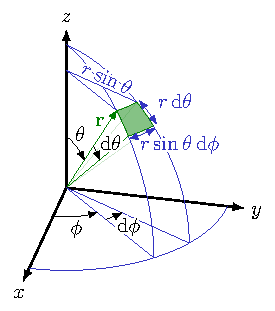
\includegraphics[width=0.75\linewidth]{Figures/Magnetics/SphericalCoordinates_Reversed.pdf}
  \end{PointSix}
\end{frame}

\begin{frame}
  %http://hyperphysics.phy-astr.gsu.edu/hbase/electric/dipole.html
  \begin{PointSix}{Mathematical technicalities}
    \small Unlike cartesian coordinates, the unit vectors in polar coordinates ($\hat{\theta},\hat{\phi}$ not $\hat{r}$) are functions of positions. Therefore the derivatives take a different form in different coordinate systems.
    $$
    \nabla A = \hat{r}\frac{\partial}{\partial r} + \hat{\theta} \frac{1}{r}\frac{\partial}{\partial \theta}
    $$
    $$
    \nabla \cdot \vec{B} = \frac{1}{r^2}\frac{\partial}{\partial r}\left(r^2B_r \right)+\frac{1}{r\sin(\theta)}\frac{\partial}{\partial \theta}\left(\sin(\theta) B_\theta \right)
    $$
    \small No need to be scared. Totally doable with some exercises.
  \end{PointSix}
\end{frame}

\begin{frame}
  %http://hyperphysics.phy-astr.gsu.edu/hbase/electric/dipole.html
  \begin{PointSix}{The dipole field visualized}
    \begin{tikzpicture}
      \node[anchor=south west,inner sep=0] at (0,0) {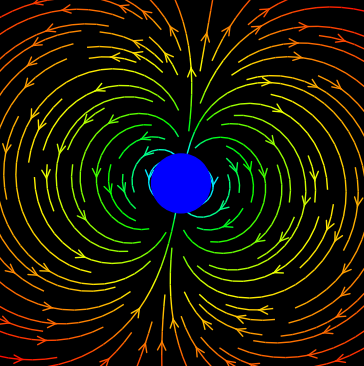
\includegraphics[width=\linewidth]{Figures/Magnetics/DipoleExported.png}};
      %\draw[red,ultra thick,rounded corners] (5,3) rectangle (9.4,6.2);
      \draw[->,line width=0.75mm,pink] (4.5,3.5) -- (5.0,6) node[midway, right] {$\vec{m}$};
    \end{tikzpicture}
  \end{PointSix}
\end{frame}
\begin{frame}
  %http://hyperphysics.phy-astr.gsu.edu/hbase/electric/dipole.html
  \begin{PointSix}{The dipole field visualized}
    \begin{tikzpicture}
      \node[anchor=south west,inner sep=0] at (0,0) {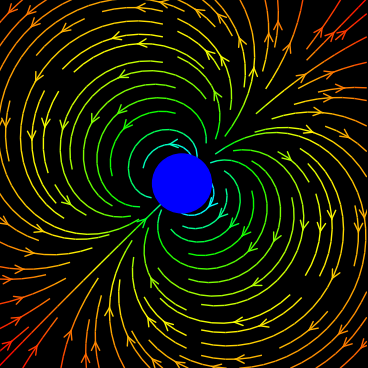
\includegraphics[width=\linewidth]{Figures/Magnetics/DipoleRot.png}};
      %\draw[red,ultra thick,rounded corners] (5,3) rectangle (9.4,6.2);
      \draw[->,line width=0.75mm,pink,rotate around={-35:(4.75,4.75)}] (4.5,3.5) -- (5.0,6) node[midway, right] {$\vec{m}$};
    \end{tikzpicture}
  \end{PointSix}
\end{frame}
\begin{frame}
  %http://hyperphysics.phy-astr.gsu.edu/hbase/electric/dipole.html
\begin{PointSix}{The dipole field visualized}
    \begin{tikzpicture}
      \node[anchor=south west,inner sep=0] at (0,0) {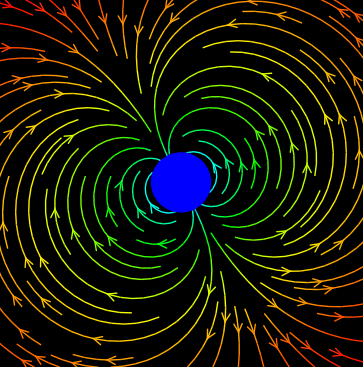
\includegraphics[width=\linewidth]{Figures/Magnetics/DipoleRot2.png}};
      %\draw[red,ultra thick,rounded corners] (5,3) rectangle (9.4,6.2);
      \draw[->,line width=0.75mm,pink,rotate around={-142:(4.75,4.75)}] (4.5,3.5) -- (5.0,6) node[midway, right] {$\vec{m}$};
    \end{tikzpicture}
  \end{PointSix}
\end{frame}

\begin{frame}
\begin{PointSix}{Dipole summary}
  \begin{itemize}
    \item The dipole approach is simplest option because there are \alert{no magnetic monopoles}. 
    \item The dipole field has closed field lines and is oriented with the dipole moment $\vec{m}$.
    \item The dipole field is the basic 'unit' in magnetics.
  \end{itemize}
\end{PointSix}
\end{frame}

\begin{frame}
  \begin{PointSix}{Fundamentals}
    What causes a magnetic field? 
    \\
    \alert{Electric currents!}
    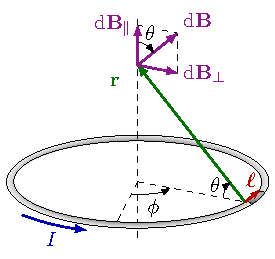
\includegraphics[width=0.8\linewidth]{Figures/Magnetics/DipoleCurrentLoop1.pdf}
  \end{PointSix}
\end{frame}

\begin{frame}
  \begin{PointSix}{Fundamentals}
    What causes a magnetic field? 
    \\
    \alert{Electric currents!}
    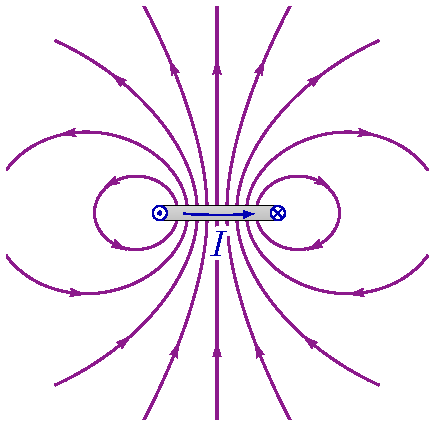
\includegraphics[width=0.8\linewidth]{Figures/Magnetics/DipoleCurrentLoopSide.pdf}
  \end{PointSix}
\end{frame}

\begin{frame}
  \begin{PointSix}{Dipole summary}
    \begin{itemize}
      \item A closed loop with a current is the source of a dipole field (and the calculation with positive/magnetic monopoles is a trick that makes it easier. Alternatively use Bio-Savart or a multipole expansion.)
    \end{itemize}
  \end{PointSix}
  \end{frame}

  \begin{frame}
    \begin{PointSix}{Magnetic field of the Earth}
      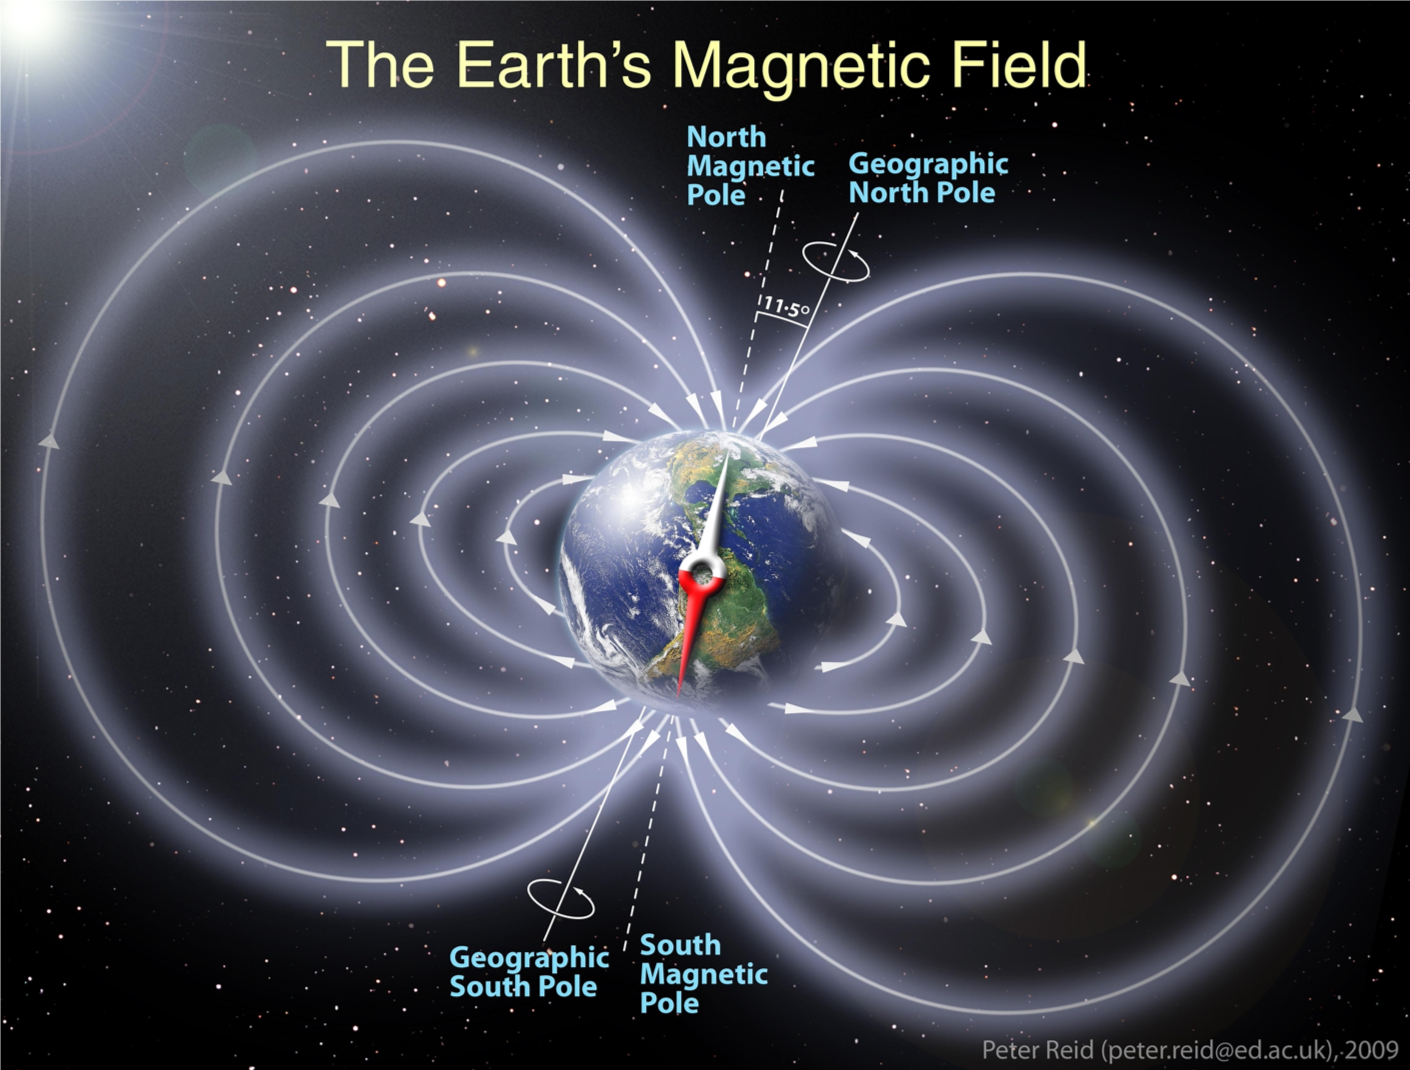
\includegraphics[width=0.99\linewidth]{Figures/Magnetics/MagneticFieldEarth_PReid_Edinburgh.png}

      \tiny [P. Reid, Univ. Edinburgh, UK]
    \end{PointSix}
  \end{frame}


  \begin{frame}
    \begin{PointSix}{Magnetic field of the Earth}
      \begin{itemize}
        \item Earth's magnetic field is to a good approximation a dipole field (in the absence of near-surface anomalies).
        \item The origin of this field is deep in Earth's interior (conduction currents in outer mantel).
        \item The dipole moment is not parallel to rotation axis but shift. Hence there is an offset between magnetic and geographic poles.
      \end{itemize}
    \end{PointSix}
    \end{frame}

    \begin{frame}
    \begin{PointSix}{Magnetic field of the Earth}
      \begin{itemize}
        \item North seeking end of magnetic needles dips downwards in northern hemisphere.
        \item South seeking end of magnetic needles dips downwards in southern hemisphere.
      \end{itemize}
    \end{PointSix}
    \end{frame}

    \begin{frame}
      \begin{PointSix}{Magnetic field of the Earth}
        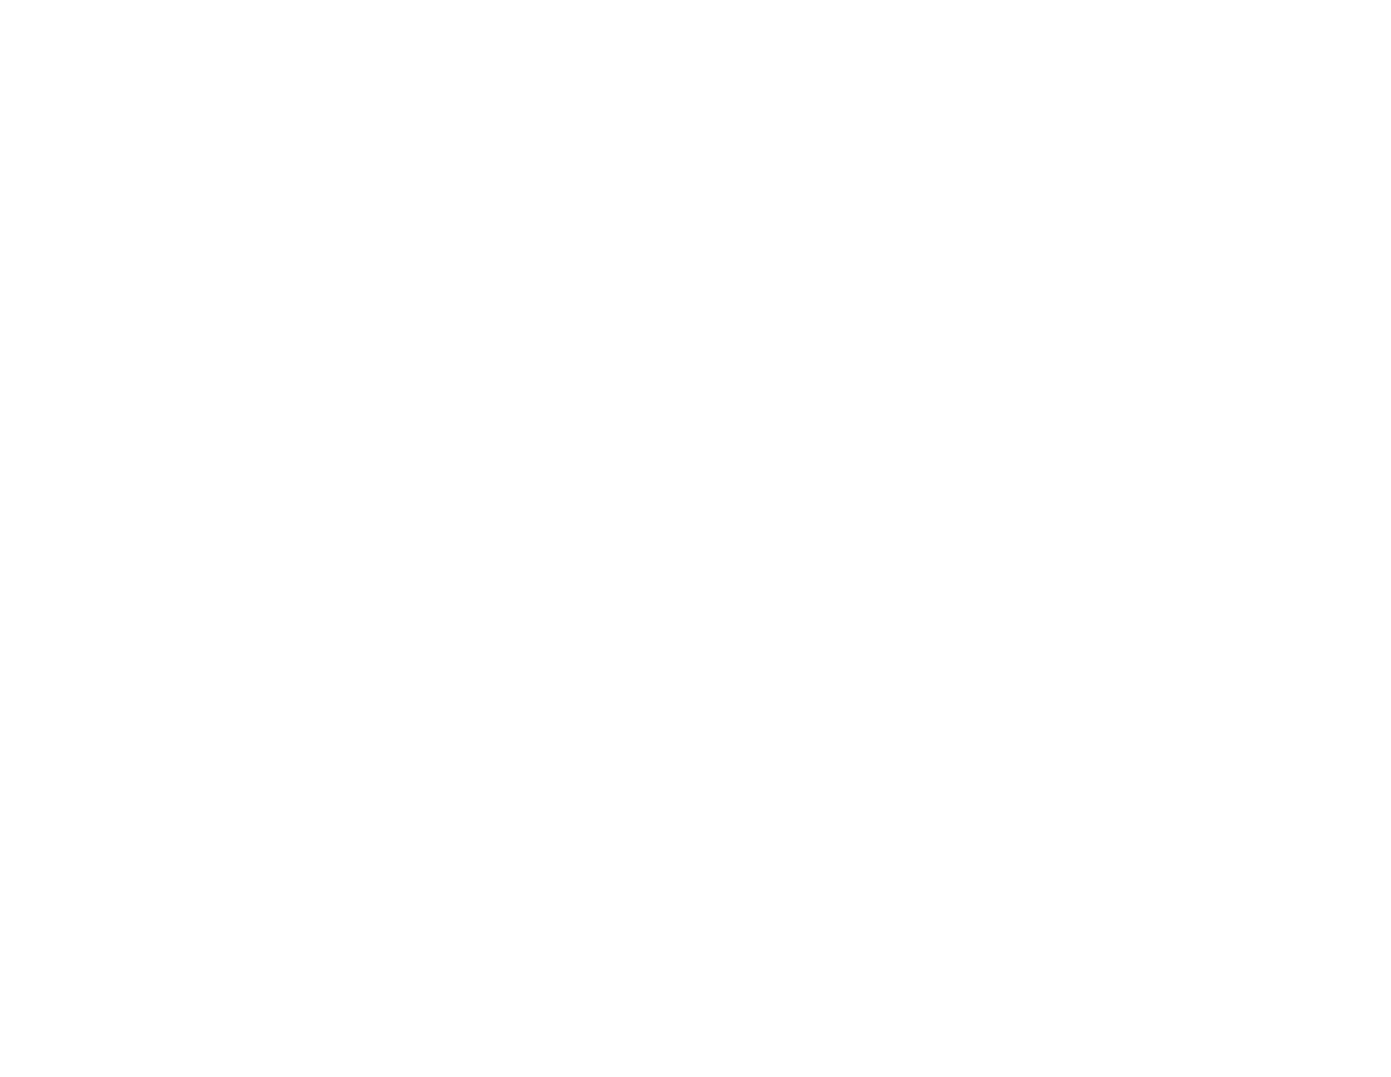
\includegraphics[width=0.99\linewidth]{Figures/Magnetics/Coordinates.png}
      \end{PointSix}
    \end{frame}

    \begin{frame}
      \begin{PointSix}{Magnetic field of the Earth}
        \small
          T: total field ($T^2=H^2+Z^2=X^2+Y^2+Z^2)$ \\
          Z: vertical component of T \\
          X: component of T in geographic N-S direction \\
          Y: component of T in geographic W-E direction \\
          H: horizontal component of T \\
          I: inclination (angle versus horizontal) \\
          D: declination (angle versus geographic N) \\
      \end{PointSix}
    \end{frame}

    \begin{frame}
      
        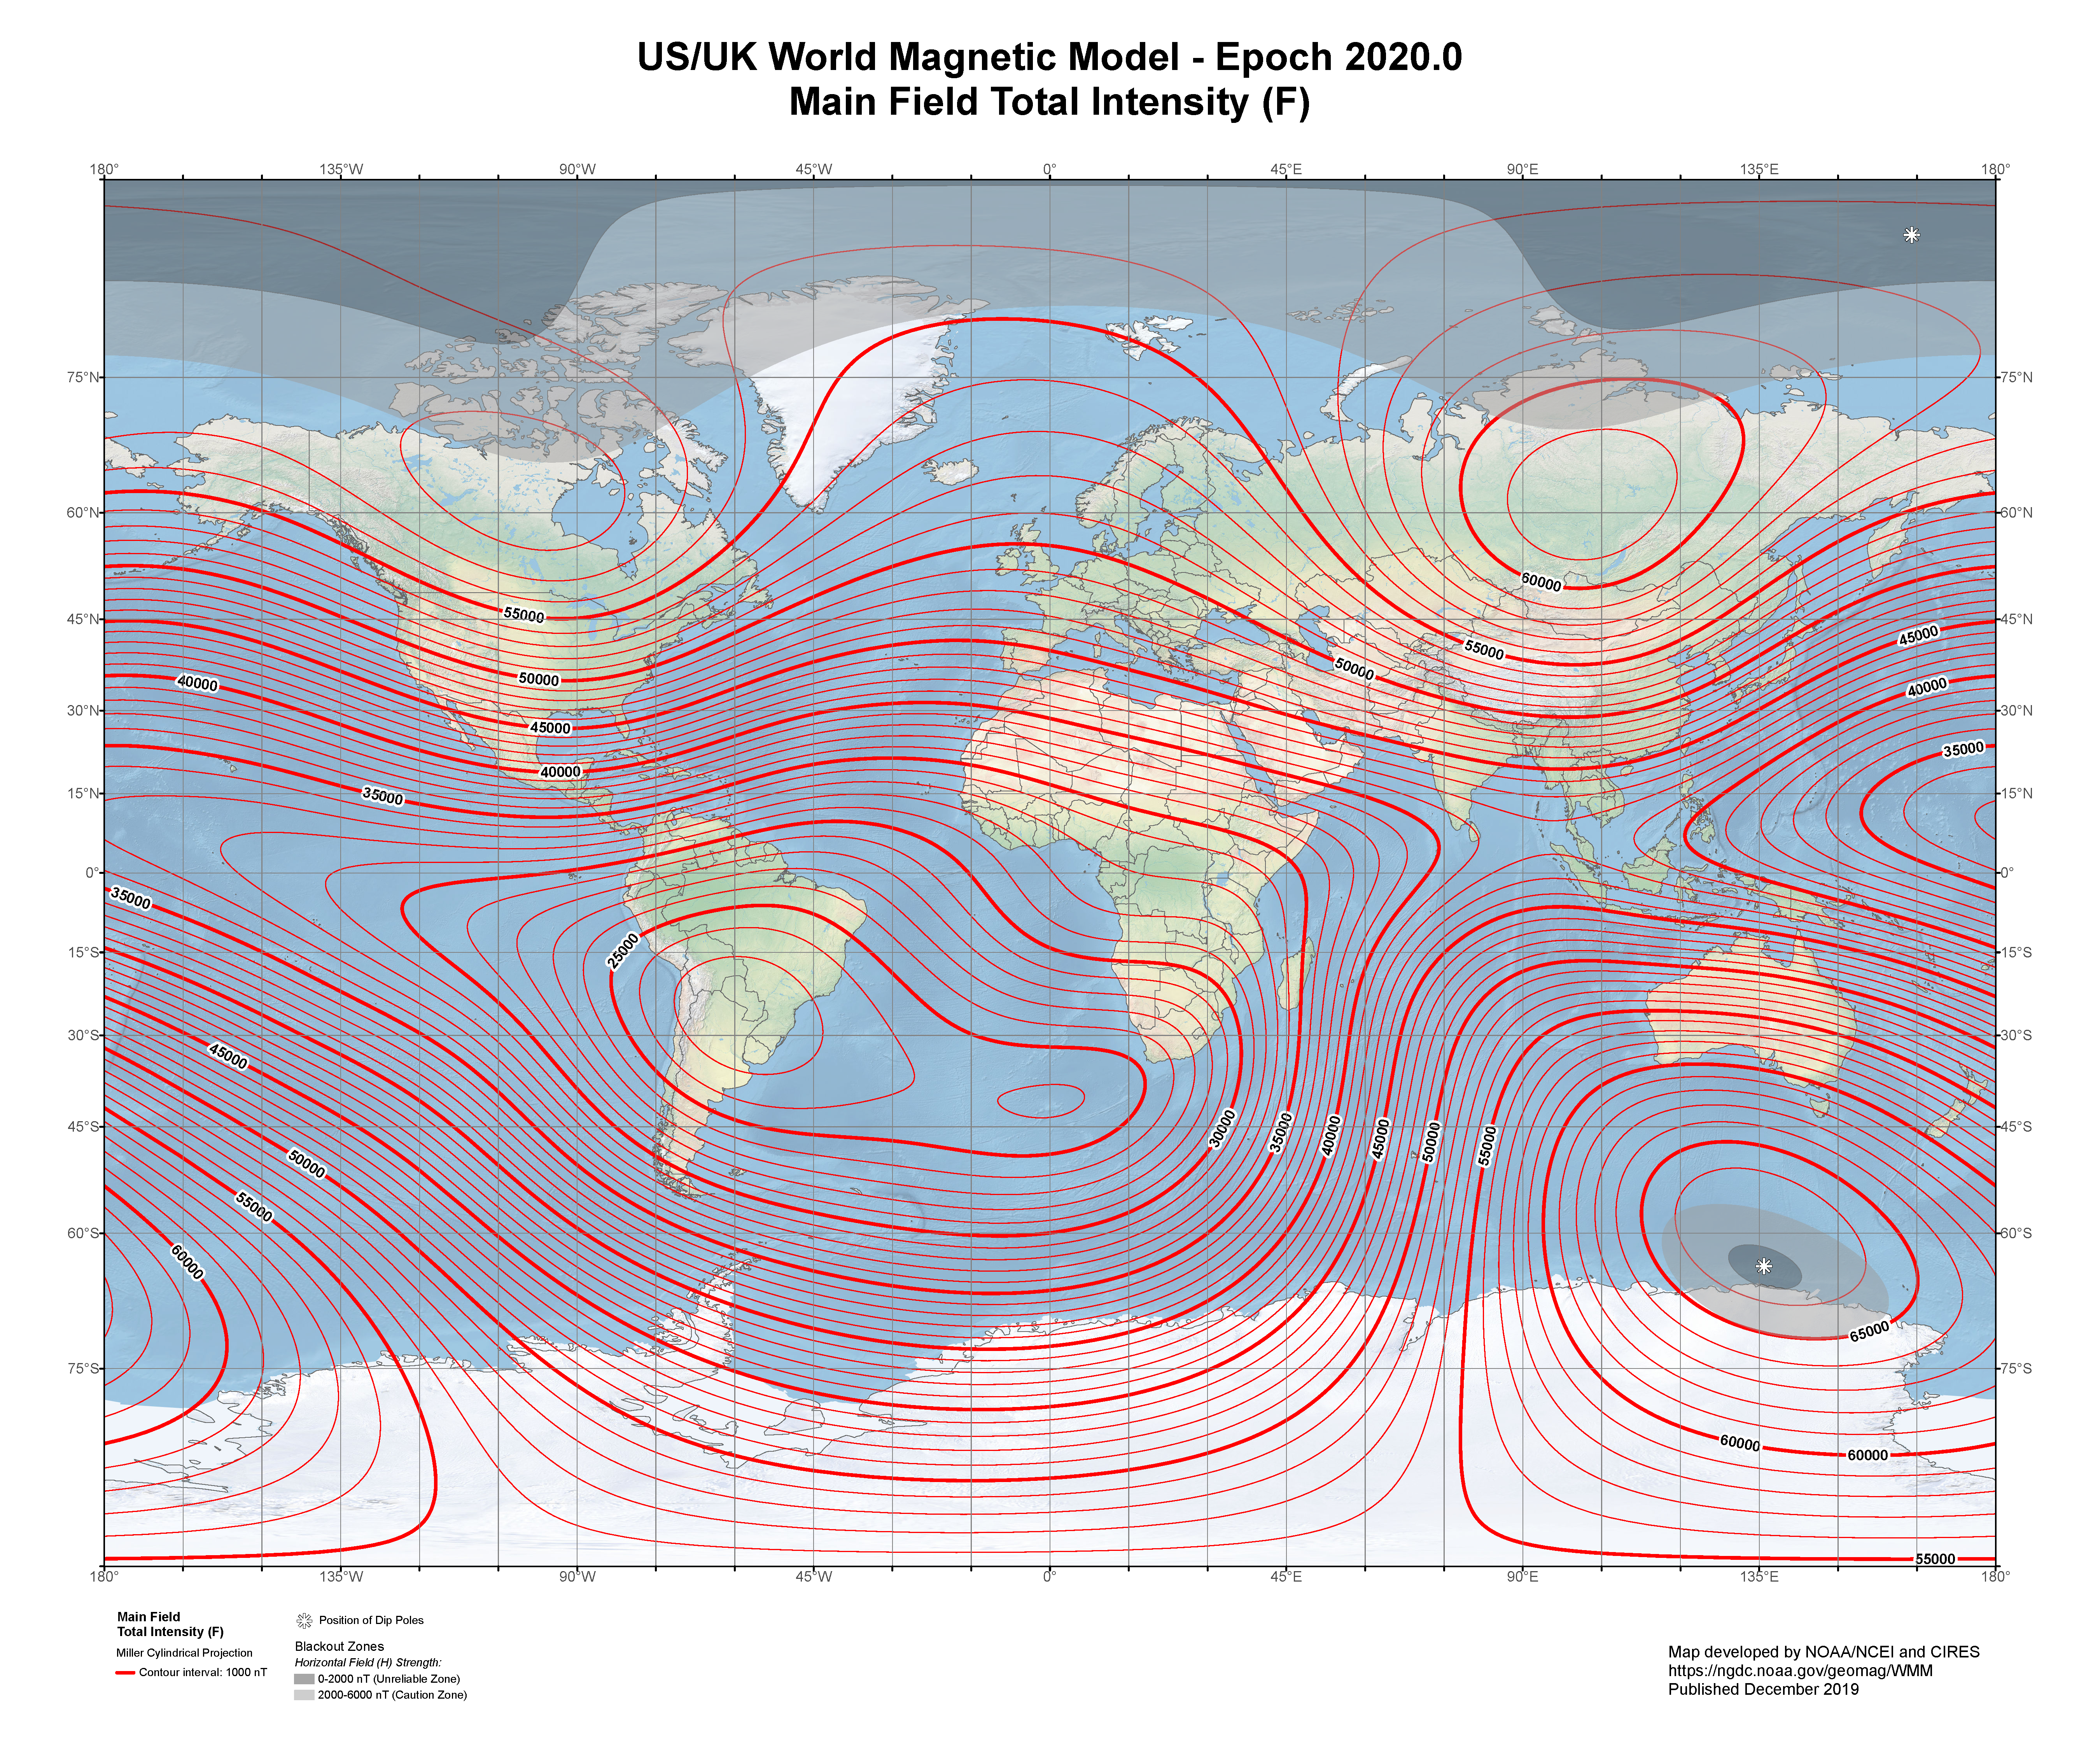
\includegraphics[width=0.75\linewidth]{Figures/Magnetics/WMM2020_F_BoZ_MILL.pdf}

    
    \end{frame}

    \begin{frame}
        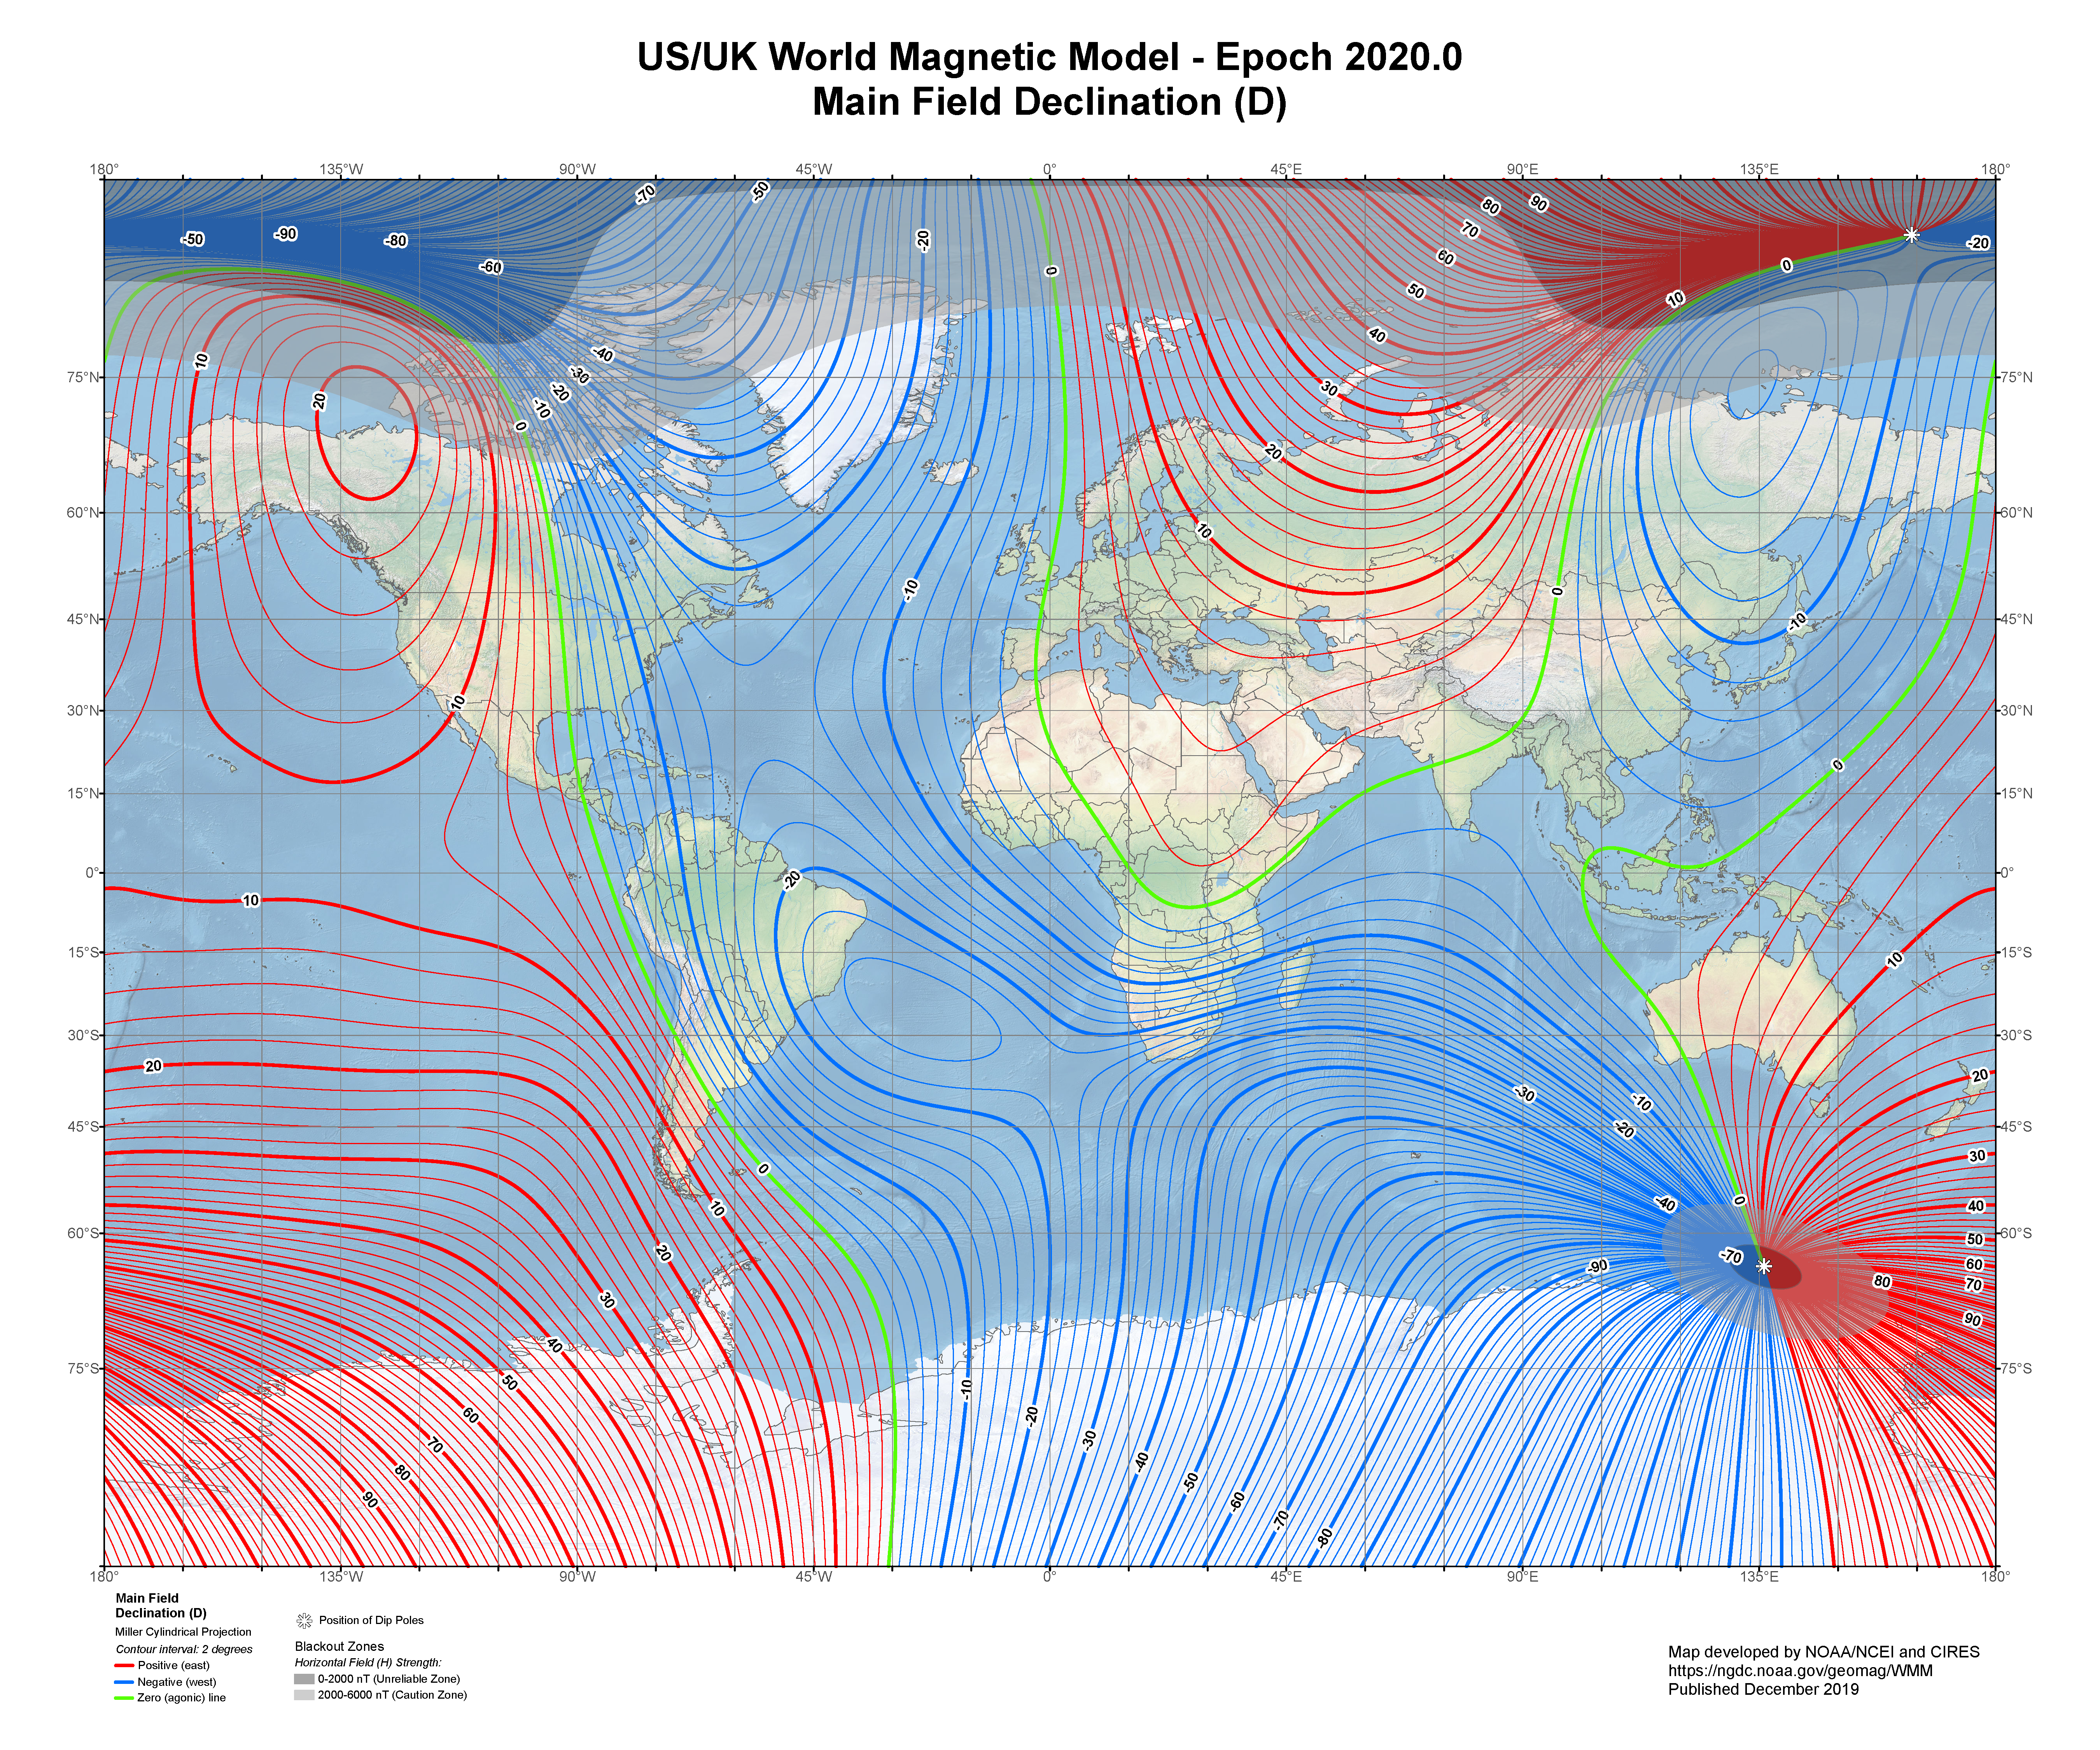
\includegraphics[width=0.75\linewidth]{Figures/Magnetics/WMM2020_D_BoZ_MILL.pdf}
    \end{frame}

    \begin{frame}
      \begin{PointSix}{Magnetic field of the Earth}
        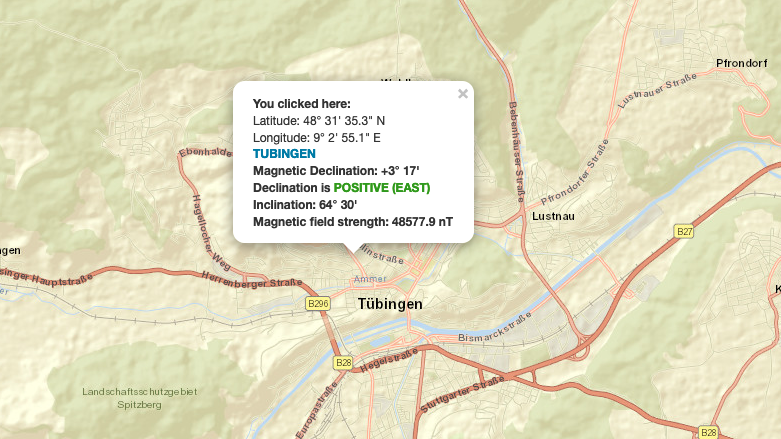
\includegraphics[width=0.99\linewidth]{Figures/Magnetics/MagnticFieldTuebingen.png}

        [Tübingen $T \sim 49 000 nT$]
      \end{PointSix}
    \end{frame}

    \begin{frame}
      \begin{PointSix}{Magnetic field of the Earth}
        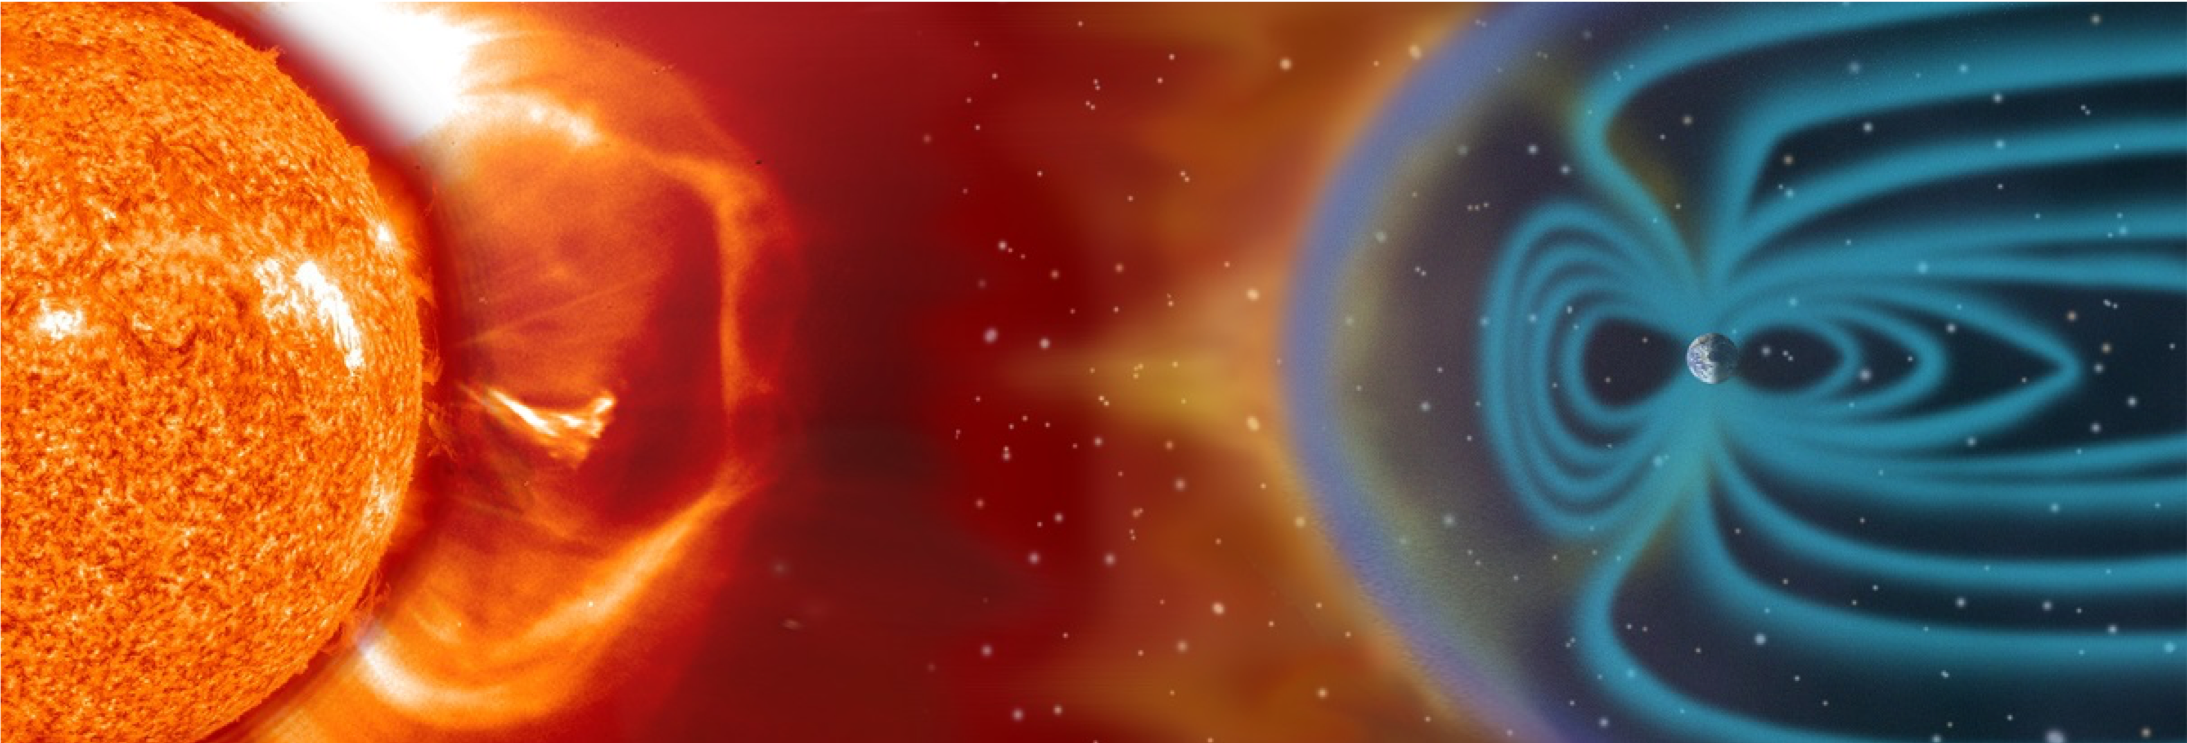
\includegraphics[width=0.99\linewidth]{Figures/Magnetics/SolarStorms.png}

        \tiny [NASA]
        \small
        \begin{itemize}
          \item The Earth's magnetic field is time variable, on contemporary timescales because of solar storms. Space weather is a real thing and can be detected, e.g., with GPS measurements. A reference station in magnetics is more important than in the gravity method.
        \end{itemize}
      \end{PointSix}
    \end{frame}

    \begin{frame}
      \begin{PointSix}{Magnetic field of the Earth}
        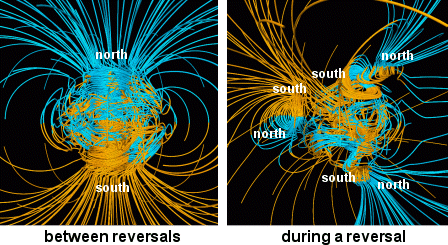
\includegraphics[width=0.99\linewidth]{Figures/Magnetics/NASA_54559main_comparison1_strip.png}

        \tiny [Model of Glatzmeier \& Roberts ]
        \small
        \begin{itemize}
          \item Magnetic pole reversal and shifts on longer timescales. Great technique for dating!
        \end{itemize}
      \end{PointSix}
    \end{frame}
  
    \begin{frame}
      \begin{PointSix}{Differentiation between $\vec{H}$ and $\vec{B}$}
         \begin{itemize}
          \item $\vec{H}$ is the \textit{magentizing field} 
          \item $\vec{B}$ is the \textit{magnetic induction}
          \item What's the difference?
        \end{itemize}
      \end{PointSix}
    \end{frame}

    \begin{frame}
      \begin{PointSix}{Induced Magnetization}
        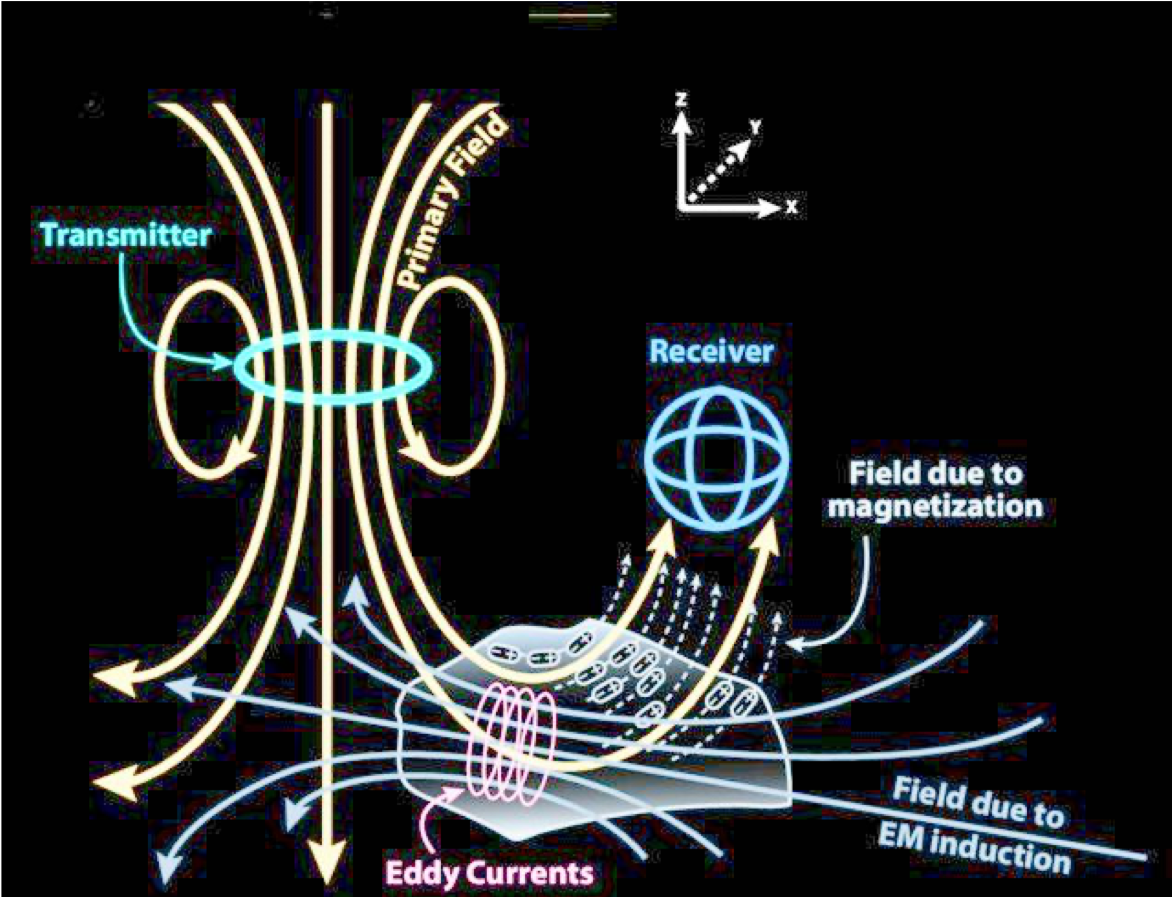
\includegraphics[width=0.90\linewidth]{Figures/Magnetics/HBInduction_GrandAndWest1995_DrawingKulvonen.png}

        \tiny [Modified from Grant and West 1965; drawing Harri Kutvonen, GTK]

      \end{PointSix}
    \end{frame}

    \begin{frame}
      \begin{PointSix}{Induced Magnetization}
        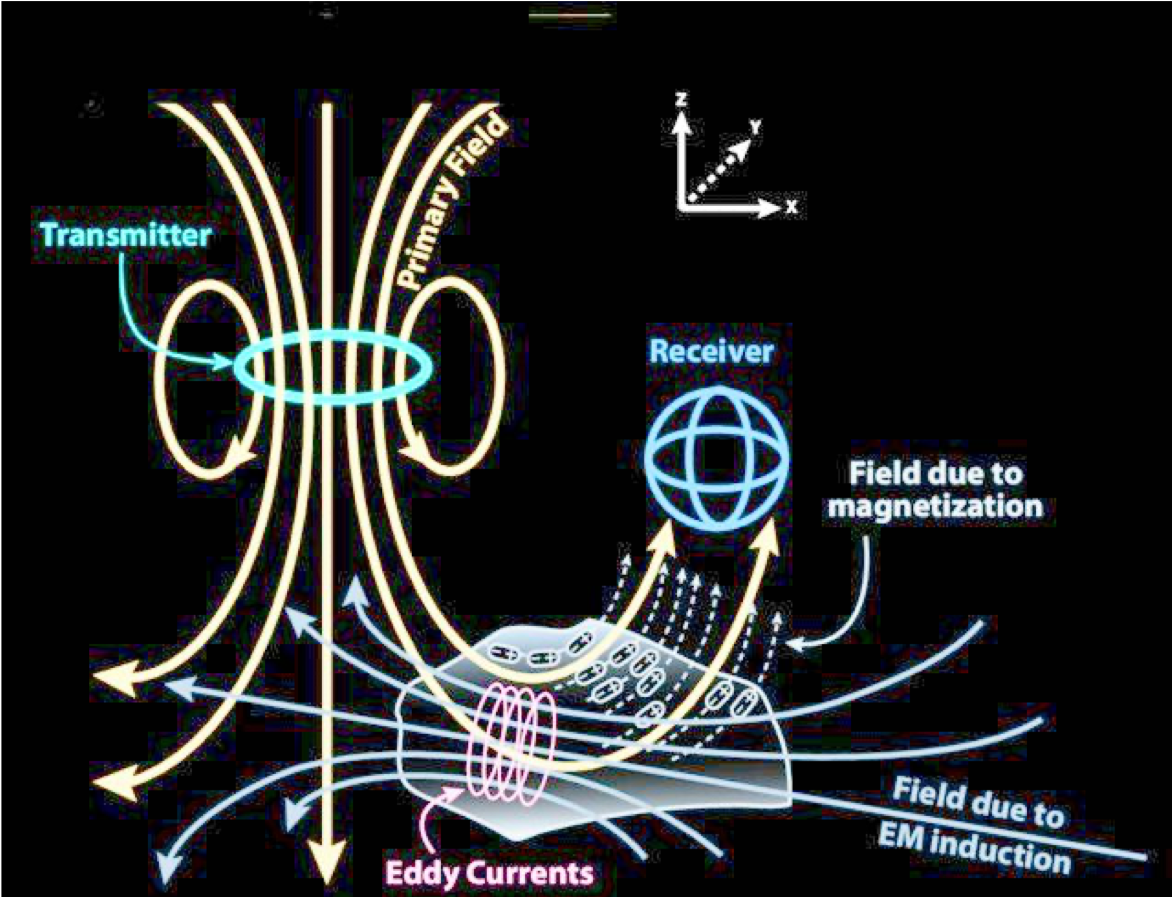
\includegraphics[width=0.6\linewidth]{Figures/Magnetics/HBInduction_GrandAndWest1995_DrawingKulvonen.png}
        \tiny [Modified from Grant and West 1965; drawing Harri Kutvonen, GTK]

        \small
        \begin{itemize}
          \item An external field ($\vec{H}$) can magnetize material so that it develops a \textit{macroscopic} magnetization intensity $\vec{M}_i = \frac{d\vec{m}_i}{dV}$ 
        \end{itemize}
      \end{PointSix}
    \end{frame}

    \begin{frame}
      \begin{PointSix}{Induced Magnetization}
        The orientation and degree of magnetization is material dependent:
        $$
          \vec{M} = \chi \vec{H}
        $$
        $\chi$ is the magnetic susceptibility. It differs from material to material (i.e. rock types etc).
      \end{PointSix}
    \end{frame}

    \begin{frame}
      \begin{PointSix}{Induced Magnetization}
        The orientation and degree of magnetization is material dependent:
        $$
          \vec{M} = \chi \vec{H}
        $$
        $\chi$ is the magnetic susceptibility. It differs from material to material (i.e. rock types etc).
      \end{PointSix}
    \end{frame}

    \begin{frame}
      \begin{PointSix}{Differentiation between $\vec{H}$ and $\vec{B}$}
      The total (physically relevant) magnetic induction $\vec{B}$ is the superposition of external ($\vec{H}$) and local ($\chi \vec{M}$):
      \begin{align*}
        \vec{B} &= \mu_0\left(\vec{H} + \vec{M} \right)\\
                &= \mu_0 (1 + \chi) \vec{H} \\
                &= \mu_0 \mu \vec{H}
      \end{align*}
      $\mu \qquad \text{\small magnetic permeability}$
      $\chi \qquad \text{\small magnetic susceptibility (dimensionless)}$
      $[B]: \qquad \text{\small Tesla}$
      \end{PointSix}
    \end{frame}

    \begin{frame}
      \begin{PointSix}{Differentiation between $\vec{H}$ and $\vec{B}$}
      The total (physically relevant) magnetic induction $\vec{B}$ is the superposition of external ($\vec{H}$) and local ($\chi \vec{M}$):
      \begin{align*}
        \vec{B} &= \mu_0\left(\vec{H} + \vec{M} \right)\\
                &= \mu_0 (1 + \chi) \vec{H} \\
                &= \mu_0 \mu \vec{H}
      \end{align*}
   

      \alert{We assume that $\vec{H}$ and $\vec{M}$ are parallel! (Not always the case.)}
      \end{PointSix}
    \end{frame}


    \begin{frame}
      \begin{PointSix}{Principals of magnetic surveys}
        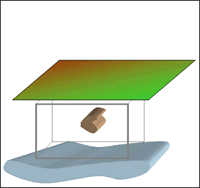
\includegraphics[width=0.80\linewidth]{Figures/Magnetics/no_field.png}

      \tiny [2017, GeoSci Developers.]
      \end{PointSix}
    \end{frame}

    \begin{frame}
      \begin{PointSix}{Principals of magnetic surveys}
        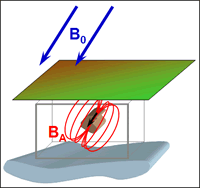
\includegraphics[width=0.80\linewidth]{Figures/Magnetics/inducing_field.png}

      \tiny [2017, GeoSci Developers.]
      \end{PointSix}
    \end{frame}

    \begin{frame}
      \begin{PointSix}{Principals of magnetic surveys}
        \includegraphics[width=0.80\linewidth]{Figures/Magnetics/inducing_field.png}

      \tiny [2017, GeoSci Developers.]
      \end{PointSix}
    \end{frame}

    \begin{frame}
      \begin{PointSix}{Principals of magnetic surveys}
        \includegraphics[width=0.80\linewidth]{Figures/Magnetics/magnetic_anomaly.png}

      \tiny [2017, GeoSci Developers.]
      \end{PointSix}
    \end{frame}

    \begin{frame}
      \begin{PointSix}{Principals of magnetic surveys}
        \includegraphics[width=0.80\linewidth]{Figures/Magnetics/measurements.png}

      \tiny [2017, GeoSci Developers.]
      \end{PointSix}
    \end{frame}

    \begin{frame}
      \begin{PointSix}{Learning Goals}
        \alert{Learning goals today:}
        \begin{itemize}
          \item Peak into applications
          \item Principals about magnetic fields (i.e., dipole field, $\vec{H}$,$\vec{B}$,$\vec{M}$,$\chi$)
          \item The Earth's magnetic field (T,H,D,I,..)
          \item The idea behind magnetic surveys.
        \end{itemize}
      \end{PointSix}
  \end{frame}  % I did this in 1 h. 
%\begin{frame}
  \begin{PointSix}{Houskeeping}
    \begin{itemize}
      \item \alert{Ask and take picture from Plenum.}
      \item \alert{Geophysics at seminar 20.05.2022}
      \item \alert{Should we do linearly varying density from Ex?}
    \end{itemize}
  \end{PointSix}
\end{frame}


\begin{frame}
    \begin{PointSix}{Learning Goals}
      \alert{Learning goals today:}
      \begin{itemize}
        \item Understand the shape of the magnetic anomalies
        \item Understand the measurement principle and sensors
        \item Understand different types of magnetism and its temperature dependency
      \end{itemize}
    \end{PointSix}
\end{frame}

\begin{frame}
  \begin{PointSix}{Remember: Differentiation between $\vec{H}$ and $\vec{B}$}
  The total (physically relevant) magnetic induction $\vec{B}$ is the superposition of external ($\vec{H}$) and local ($\chi \vec{M}$):
  \begin{align*}
    \vec{B} &= \mu_0\left(\vec{H} + \vec{M} \right)\\
            &= \mu_0 (1 + \chi) \vec{H} \\
            &= \mu_0 \mu \vec{H}
  \end{align*}
  $\mu \qquad \text{\small magnetic permeability}$
  $\chi \qquad \text{\small magnetic susceptibility (dimensionless)}$
  $[B]: \qquad \text{\small Tesla}$
  \end{PointSix}
\end{frame}

\begin{frame}
  \begin{PointSix}{Remember: Differentiation between $\vec{H}$ and $\vec{B}$}
  \alert{In geomagnetics, the magnetic susceptibility is the parameter that we are after.}
  \begin{align*}
    \vec{B} &= \mu_0\left(\vec{H} + \vec{M} \right)\\
            &= \mu_0 (1 + \chi) \vec{H} \\
            &= \mu_0 \mu \vec{H}
  \end{align*}
  $\mu \qquad \text{\small magnetic permeability}$
  $\chi \qquad \text{\small magnetic susceptibility (dimensionless)}$
  $[B]: \qquad \text{\small Tesla}$
  \end{PointSix}
\end{frame}

\begin{frame}
  \begin{PointSix}{Principals of magnetic surveys}
    \includegraphics[width=0.80\linewidth]{Figures/Magnetics/inducing_field.png}

  \tiny [2017, GeoSci Developers.]
  \end{PointSix}
\end{frame}

\begin{frame}
  \begin{PointSix}{Principals of magnetic surveys}
    \includegraphics[width=0.80\linewidth]{Figures/Magnetics/inducing_field.png}

  \tiny [2017, GeoSci Developers.]
  \end{PointSix}
\end{frame}

\begin{frame}
  \begin{PointSix}{Principals of magnetic surveys}
    \includegraphics[width=0.80\linewidth]{Figures/Magnetics/magnetic_anomaly.png}

  \tiny [2017, GeoSci Developers.]
  \end{PointSix}
\end{frame}

\begin{frame}
  \begin{PointSix}{Principals of magnetic surveys}
    \includegraphics[width=0.80\linewidth]{Figures/Magnetics/measurements.png}

  \tiny [2017, GeoSci Developers.]
  \end{PointSix}
\end{frame}



\begin{frame}
    \begin{PointSix}{Strategy for expectations of induced magentic dipoles}
      \alert{Induced magnetic dipole:=Direction of $\vec{m} \parallel \vec{B}_0$}
      \small
      \begin{itemize}
        \item Draw S-End, N-End and inclination of planned profile
        \item Draw $\vec{m}$ and corresponding dipole field at depth
        \item Analyse superposition of $B_0$ and dipolfield. 
        \item (Assume that the anomaly is essentially parallel to $B_0$)
      \end{itemize}
    \end{PointSix}
\end{frame}

\begin{frame}
  \begin{PointSix}{Induced magnetization examples}
    \includegraphics[width=0.7\textwidth]{Figures/Magnetics/AlmostParallel.png}

    [Soengonkono Intect 2015)]
  \end{PointSix}
\end{frame}

\begin{frame}
    \begin{PointSix}{Induced magnetization examples}
      \includegraphics[width=0.9\textwidth]{Figures/Magnetics/AnomalyMagneticEquator.png}

      [Soengonkono Intect 2015)]
    \end{PointSix}
\end{frame}

\begin{frame}
    \begin{PointSix}{Induced magnetization examples}
      \includegraphics[width=0.9\textwidth]{Figures/Magnetics/AnomalyMagneticSouthPole.png}

      [Soengonkono Intect 2015)]
    \end{PointSix}
\end{frame}

\begin{frame}
    \begin{PointSix}{Induced magnetization examples}
      \includegraphics[width=0.9\textwidth]{Figures/Magnetics/AnomalySouthernHemisphere.png}

      [Soengonkono Intect 2015)]
    \end{PointSix}
\end{frame}

\begin{frame}
    \begin{PointSix}{Induced magnetization examples}
      \includegraphics[width=0.9\textwidth]{Figures/Magnetics/AnomalyNothernHemisphere.png}

      [Soengonkono Intect 2015)]
    \end{PointSix}
\end{frame}

\begin{frame}
  \begin{PointSix}{Interpreting magnetic anomalies:}
    \begin{itemize}
      \item Unlike in gravity, magnetic can be measured in 3D
      \item Interpretation of $\Delta T$, $\Delta H$, $\Delta Z$, ...
      \item Commonly also the vertical gradient of $\Delta Z$ (cf. exercises)
    \end{itemize}
  \end{PointSix}
\end{frame}

\begin{frame}
  \begin{PointSix}{Demonstration of foreward model}
    \includegraphics[width=0.9\textwidth]{Figures/Magnetics/MagneticAnomalyAllComponents.png}


  \end{PointSix}
\end{frame}


\begin{frame}
  \begin{PointSix}{Demonstration of foreward model}
    \includegraphics[width=0.9\textwidth]{Figures/Magnetics/GeoXYZ_Setup.png}


  \end{PointSix}
\end{frame}

\begin{frame}
  \begin{PointSix}{Demonstration of foreward model}
    \includegraphics[width=0.9\textwidth]{Figures/Magnetics/GeosciXYZ_MagneticApplet.png}


  \end{PointSix}
\end{frame}

\begin{frame}
  \begin{PointSix}{Half-width rules}
   Similar to the anomaly in gravity surveys, we can also apply a half-width rule in magnetics to estimate the depth of the object. 

   $$
    d \sim HW
   $$

   Check this with the forward model.
  \end{PointSix}
\end{frame}







\begin{frame}
  \begin{PointSix}{Types of Magnetometers: Proton Precession}
    \includegraphics[width=0.8\textwidth]{Figures/Magnetics/LamorPrecession_XSnelgrove.png}

    \tiny [XSnelgrove (CC-BY-SA 2.5)]
  \end{PointSix}
\end{frame}

\begin{frame}
  \begin{PointSix}{Types of Magnetometers: Proton Precession}
  \small
    \begin{itemize}
      \item Hydrogen atoms have angular momentum (spin) and magnetic moment (moved charge). Both are vectors which are parallel to each other and linked by the gyromagnetic ratio ($\gamma_p$).
    \end{itemize}
  \end{PointSix}
\end{frame}

\begin{frame}
  \begin{PointSix}{Types of Magnetometers: Proton Precession}
    \small
    \begin{itemize}
      \item Protons have angular momentum and magnetic moment.
      \item External magnetic field induces torque, so that mini magnetic moment tends to aligns parallel to the external field.
    \end{itemize}
  \end{PointSix}
\end{frame}

\begin{frame}
  \begin{PointSix}{Types of Magnetometers: Proton Precession}
    \small
    \begin{itemize}
      \item Hydrogen atoms have angular momentum and magnetic moment.
      \item External magnetic field induces torque, alignment near parallel to external field.
      \item Because of internal spin, this torque induces precession (analogy to spinning top).
    \end{itemize}
  \end{PointSix}
\end{frame}

\begin{frame}
  \begin{PointSix}{Types of Magnetometers: Proton Precession}
    \small
    \begin{itemize}
      \item Hydrogen atoms have angular momentum and magnetic moment.
      \item External magnetic field induces torque, alignment near parallel to external field.
      \item Because of internal spin, this torque induces precession (analogy to spinning top).
      \item The precession frequency $\omega$ is sensitive to the \textit{total external field}, not its direction. 
    \end{itemize}
    $$
      \omega = \gamma_p |B|
    $$
  \end{PointSix}
\end{frame}

\begin{frame}
  \begin{PointSix}{Types of Magnetometers: Proton Precession}
    \small
    \begin{itemize}
      \item Hydrogen atoms have angular momentum and magnetic moment.
      \item External magnetic field induces torque, alignment near parallel to external field.
      \item Because of internal spin, this torque induces precession (analogy to spinning top).
      \item The precession frequency $\omega$ is sensitive to the \textit{total external field}, not its direction. 
      \item \alert{Idea: Measure $\omega$ and infer $|B|$}
    \end{itemize}
    $$
      \omega = \gamma_p |B|
    $$
  \end{PointSix}
\end{frame}

\begin{frame}
  \begin{PointSix}{Types of Magnetometers: Proton Precession}
    \small
    \alert{Practical implementation:}
    \begin{itemize}
      \item Use liquid with many hydrogen atoms (e.g. water or kerosene).
      \item Align their magnetic moments with strong, external magnetic field.
    \end{itemize}
  \end{PointSix}
\end{frame}


\begin{frame}{Types of Magnetometers: Fluxgate}
  %\begin{PointSix}{Induced magnetization examples}
    \includegraphics[width=0.8\textwidth]{Figures/Magnetics/ProtonPrecessionSpinAlignment_FOrdonez2014.png}
    
    \tiny [F. Ordonez 2014]

    \alert{\small At room temperatures spins are not aligned as Earth's magnetic field is too weak to do so.}
  %\end{PointSix}
\end{frame}

\begin{frame}
  \begin{PointSix}{Types of Magnetometers: Proton Precession}
    \small
    \alert{Practical implementation:}
    \begin{itemize}
      \item Use liquid with many hydrogen atoms (e.g. water or kerosene).
      \item Align their magnetic moments with strong, external magnetic field.
      \item Measure the precession frequency (how?)
    \end{itemize}
  \end{PointSix}
\end{frame}

\begin{frame}{Induction: Time variable $B$ field induce currents}
  \centering
  \animategraphics[loop,width=9cm]{10}{Figures/Magnetics/animation/Electromagnetic_induction_Ponor-}{0}{20}

  \tiny [Animation by Ponor (CC-BY-SA)]
\end{frame}

\begin{frame}{Induction: Time variable $B$ field induce currents}
  $$
    \varepsilon = \frac{d\phi_B}{dt}
  $$
  \begin{itemize}
    \item $\varepsilon$ electromotive force (e.g., leads to current in coil)
    \item $\phi_B$ intercepted magnetic flux 
  \end{itemize}

\end{frame}

\begin{frame}{Induction: Time variable $B$ field induce currents}
  $$
    \varepsilon = \frac{d\phi_B}{dt}
  $$
  \begin{itemize}
    \item $\varepsilon$ electromotive force (e.g., leads to current in coil)
    \item $\phi_B$ intercepted magnetic flux 
    \item Faraday's law of induction
  \end{itemize}
  $$
    \nabla \times \vec{E} = -\frac{\partial}{\partial t}\vec{B}
  $$

\end{frame}

\begin{frame}
  \begin{PointSix}{Types of Magnetometers: Proton Precession}
    \includegraphics[width=0.85\textwidth]{Figures/Magnetics/ProtonPrecesssion_Huggard1970.jpg}

    \tiny [Huggard 1970]
  \end{PointSix}
\end{frame}

\begin{frame}
  \begin{PointSix}{Types of Magnetometers: Proton Precession}
    \includegraphics[width=0.5\textwidth]{Figures/Magnetics/ProtonPrecession_Gemsys2012.png}

    \tiny [Gemsys 2012]
  \end{PointSix}
\end{frame}

\begin{frame}
  \begin{PointSix}{Types of Magnetometers: Proton Precession}
  \small
    \begin{itemize}
      \item Measures total field (alignment of sensor less important).
      \item Based on magnetic moment of hydrogen atom and larmor precession.
      \item Alignment in artificial external $B$ field.
      \item Measure relaxation and larmor precession via induction in surrounding coils.
      \item Sensitivity $\sim 0.1 nT$.
      \item Principals are similar to MRI
    \end{itemize}
  \end{PointSix}
\end{frame}



\begin{frame}{Types of Magnetometers: Fluxgate}
  % \begin{PointSix}{Induced magnetization examples}
     \includegraphics[width=0.8\textwidth]{Figures/Magnetics/Fluxgate_PDornelCCBYSA.png}
 
     \tiny [PDornel (CC-BY-SA)]
  % \end{PointSix}
 \end{frame}

 \begin{frame}
  \begin{PointSix}{Fluxgate magnetometer}
   \begin{itemize}
    \item Induce low-frequencey (kHz) current in primary circuit.
    \item The magnetic fields in secondary coil will be balanced \alert{in absence of external field.}
    \item External field causes imbalance between primary and secondary coils that can be used to measure $B_x$, $B_y$, $B_z$ \alert{depending on coil orientation.}
   \end{itemize}
  \end{PointSix}
\end{frame}


\begin{frame}{Types of Magnetometers: Fluxgate}
  \begin{tikzpicture}
    \node (fig1) at (0,0) {\includegraphics[scale=0.5]{Figures/Magnetics/Fluxgate_PDornelCCBYSA.png}};
    \draw [<-, line width=0.75mm, red](-3,0.6) -- (0,0.6);
    \draw [->, line width=0.75mm, red](-3,-1.5) -- (0,-1.5);
  \end{tikzpicture}
 \end{frame}

 \begin{frame}{Types of Magnetometers: Fluxgate}
  \begin{tikzpicture}
    \node (fig1) at (0,0) {\includegraphics[scale=0.5]{Figures/Magnetics/Fluxgate_PDornelCCBYSA.png}};
    \draw [<-, line width=0.75mm, red](-3,0.6) -- (-0.5,0.6);
    \draw [->, line width=0.75mm, red](-3,-1.5) -- (0.5,-1.5);
    \draw [->, line width=0.75mm, blue](-3,3) -- (4,-3);
  \end{tikzpicture}
 \end{frame}

 \begin{frame}{Types of Magnetometers: Optically pumped}
  % \begin{PointSix}{Induced magnetization examples}
     \includegraphics[width=0.8\textwidth]{Figures/Magnetics/OpticallyPumped_PDornel.png}
 
     \tiny [PDornel (CC-BY-SA)]
  % \end{PointSix}
 \end{frame}

\begin{frame}
  \begin{PointSix}{Gradiometry: Measure the vertical gradient}
   \begin{itemize}
    \item Install two sensors at different heights (e.g., 0.5 m apart).
    \item Consider only the vertical gradient.
    \item Insensitive to the total field and temporal variability thereof.
    \item Sensitive to near-surface structures (why?).
    \item Sensitive to horizontal boundaries.
    \item \alert{Relevant for applied exercises.}
   \end{itemize}
  \end{PointSix}
\end{frame}



\begin{frame}
  \begin{center}
    \includegraphics[width=0.7\linewidth]{Figures/Magnetics/ParaDiaFerro_Lacovacci2016.png}
  
    \tiny[Lacovacci2016]

    \vspace{2cm}
    
    \normalsize How do materials react to application of an external magnetic field?
  \end{center}
\end{frame}

\begin{frame}
  \begin{center}
    \includegraphics[width=0.7\linewidth]{Figures/Magnetics/ParaDiaFerro_Lacovacci2016.png}
  
    \tiny[Lacovacci2016]

    \vspace{0.24cm}
    
    \normalsize Diamagnetism
    \small 
    \begin{itemize}
      \item \alert{Weak} mini-dipoles induced, opposing external field ($\chi < 0$).
      \item Diappears if external field is removed.
      \item Occurs essentially in all materials, but is not noted everywhere, due to other effects. 
      \item Examples: Quarzite, Calcite, ...
    \end{itemize}
    
  \end{center}
\end{frame}

\begin{frame}
  \begin{center}
    \includegraphics[width=0.7\linewidth]{Figures/Magnetics/ParaDiaFerro_Lacovacci2016.png}
  
    \tiny[Lacovacci2016]

    \vspace{0.24cm}
    
    \normalsize Paramagnetism
    \small 
    \begin{itemize}
      \item Material exhibits \alert{pre-existing} dipoles which orient themselves in external field (unpaired electrons).
      \item \alert{Reinforce} external field ($\chi > 0$). 
      \item Effect dissipates due to thermal fluctuations once external field is removed.
      \item Examples: gold, copper,...
    \end{itemize}
    
  \end{center}
\end{frame}

\begin{frame}
  \begin{center}
    \includegraphics[width=0.7\linewidth]{Figures/Magnetics/ParaDiaFerro_Lacovacci2016.png}
  
    \tiny[Lacovacci2016]

    \vspace{0.24cm}
    
    \normalsize Ferromagnetism
    \small 
    \begin{itemize}
      \item Material exhibits \alert{pre-existing} dipoles which are oriented in domains with strong coupling.
      \item Domains align and \alert{strongly reinforce} external field ($\chi >> 0$). 
      \item Effect can be maintained if external field is removed.
      \item Examples: iron, nickel, ...
    \end{itemize}
    
  \end{center}
\end{frame}


\begin{frame}
  \begin{PointSix}{Temperature dependency}
    $$
      \chi = \frac{M}{H} = \frac{C}{T}
    $$
    \small
    \begin{itemize}
      \item $C$ is the Curie Constant.
      \item Overall, magnetic susceptibility decreases with increasing temperature.
    \end{itemize}
  \end{PointSix}
\end{frame}

\begin{frame}
  \begin{PointSix}{Temperature dependency}
    $$
      \chi \sim  \frac{1}{T - T_c}
    $$
    \small
    \begin{itemize}
      \item At the Curie Temperature materials loose their permanent magnetic properties.
    \end{itemize}
  \end{PointSix}
\end{frame}


\begin{frame}
  \begin{PointSix}{Learning Goals}
    \alert{Learning goals today:}
    \begin{itemize}
      \item Understand the shape of the magnetic anomalies
      \item Understand the measurement principle and sensors
      \item Understand different types of magnetism and its temperature dependency
    \end{itemize}
  \end{PointSix}
\end{frame}

 
\begin{frame}
  \begin{PointSix}{Houskeeping}
    \begin{itemize}
      \item \alert{Geophysics at seminar 20.05.2022}
      \item \alert{Questions regarding exercises}
    \end{itemize}
  \end{PointSix}
\end{frame}

\begin{frame}
  \begin{PointSix}{Learning Goals}
    \begin{itemize}
      \item \alert{Resistivity..}
      \item \alert{Currents..}
      \item \alert{Electric Fields..}
    \end{itemize}
  \end{PointSix}
\end{frame}

\begin{frame}
  \begin{PointSix}{Resistivity Method Principles}
      \small
      Characterize the sub-surface in it's ability to conduct electrical currents. A material that has a high electrical resistivity will conduct electrical currents poorly and vice versa.
  \end{PointSix}
\end{frame}

\begin{frame}
  \begin{PointSix}{Primary parameter of the resistivity method}
   % RESISTOR with battery and arrow

    \begin{tikzpicture}
      
      \newcommand\EMF{\mathcal{E}};
      \colorlet{Icol}{blue!50!black}
      \colorlet{Ccol}{orange!90!black}
      \colorlet{Rcol}{Karminrot}
      \colorlet{loopcol}{red!90!black!25}
      \colorlet{pluscol}{red!60!black}
      \colorlet{minuscol}{blue!60!black}
      \tikzstyle{EMF}=[battery1,l=$\EMF$];
      \tikzstyle{internal R}=[R,color=Rcol,Rcol,l=$r$,/tikz/circuitikz/bipoles/length=30pt];
      \tikzstyle{loop}=[->,red!90!black!25];
      \tikzstyle{loop label}=[loopcol,fill=white,scale=0.8,inner sep=1];
      \tikzstyle{thick R}=[R,color=Rcol,thick,Rcol,l=$R$];
      
      \begin{scope}[rotate=-90,transform shape]
        \fill[pattern = crosshatch dots,pattern color = brown!80!red] (0.5,-0.5) rectangle ++(6,9);
        \node[rotate=90] at (0.25,1.5) {Surface};
        \draw (0,8) to [short,*-] (4,8) to[R,color=Rcol,thick,l={{{{\rotatebox[origin=c]{90}{$R$}}}}}] (4,0) to [short,-*] (0,0);
        \node[rotate=90,above] at (0,8) {$+$};
        \node[rotate=90,above] at (0,0) {$-$};
        \node[rotate=90] at (0,4) {$\Delta V$};
          %  \draw[->,red] (0.5, 2.15) --++ (1.2,0) node[midway,above=1] {current $I$};
          %  \draw[->,red] (0.5,-0.15) --++ (1.2,0) node[midway,below=1] {electron flow};
          \end{scope}
    \end{tikzpicture}
  \end{PointSix}
\end{frame}

\begin{frame}
     \begin{PointSix}{Resistivity vs. Resistance}
      \begin{center}
        \includegraphics[width=0.90\linewidth]{Figures/Resistivity/ResistanceResistivity.png}
      \end{center}
      \small
      \begin{itemize}
        \item Resistivity (spez. elektr. Widerstand) is a material property
        \item Resistance (elektr. Widerstand) includes material and geometry of the resistor
      \end{itemize}
      \end{PointSix}
\end{frame}

\begin{frame}
  \begin{PointSix}{Resistivity vs. Resistance}
   \begin{center}
     \includegraphics[width=0.90\linewidth]{Figures/Resistivity/ResistanceResistivity.png}
   \end{center}
   \small
   \begin{itemize}
     \item Resistance [Ohm, $\Omega$]
     \item Resistivity [$\Omega m$]
   \end{itemize}
   \end{PointSix}
\end{frame}

\begin{frame}
  \begin{PointSix}{Resistivity ($\rho$) vs. Conductivity ($\sigma$)}
   \begin{center}
     $$
      \rho = \frac{1}{\sigma}
     $$
   \end{center}
   \small
   \begin{itemize}
     \item Resistivity [$\Omega m$]
     \item Conductivity [$(\Omega m)^{-1}$, i.e. Siemens]
   \end{itemize}
   \end{PointSix}
\end{frame}

\begin{frame}
  \begin{PointSix}{Ionic vs. metallic conduction}
    \begin{center}
      \includegraphics[width=0.80\linewidth]{Figures/Resistivity/conductivity_physics_diagram_RGeoSciXYZ.png}
      \tiny[GeoSci XYZ]
    \end{center}
   
      
  \end{PointSix}
\end{frame}

\begin{frame}
  \begin{PointSix}{Ionic vs. metallic}
    \begin{center}
      \includegraphics[width=0.90\linewidth]{Figures/Resistivity/MetallicCondution.png}
     % \tiny[GeoSci XYZ]
    \end{center}
    \small
    \begin{itemize}
      \item \alert{Metallic conduction} uses declocalized electrons in the conduction band of metalls
      \item \alert{Ionic conduction} uses charged Ions in electrolyt 
    \end{itemize}
    \end{PointSix}
\end{frame}
\begin{frame}
  \begin{PointSix}{Ionic conduction in porous sediments}
    \begin{center}
      \includegraphics[width=0.90\linewidth]{Figures/Resistivity/ProusMedia.png}
     % \tiny[GeoSci XYZ]
    \end{center}
    \end{PointSix}
\end{frame}

\begin{frame}
  \begin{PointSix}{Ionic conduction in porous sediments}
    \small
    \begin{itemize}
      \item Increases with increasing pore space ($\phi$)
      \item Increases with increasing water saturation
      \item Increases with decreasing water resistivity ($\rho$)
    \end{itemize}
    \normalsize
    \onslide<2>{
      \begin{equation}
        \rho_t = a\rho_w\phi^{-m}s_w^{-n}
      \end{equation}
      \begin{center}
       \small (Archie's Law)
      \end{center}
      
      }
    \end{PointSix}
\end{frame}

\begin{frame}
 % \begin{PointSix}{Huge spread in material properties}
   % RESISTOR with battery and arrow
   \begin{center}
    \includegraphics[width=0.8\linewidth]{Figures/Resistivity/ResistivityMaterials.png}
    
  \end{center}
  %\end{PointSix}
\end{frame}

\begin{frame}{Current flow through the sub-surface}
  \begin{PointSix}{Current flow through the sub-surface}
    \small
    Consider a homogeneous conducting halfspace, with constant resistivity $\rho$, under an insulating medium. Let there be a point electrode at the surface
injecting a steady current I. The current flows to a distributed sink at infinity. Find the electrostatic potential, the electric field, and consequently the pattern of current flow in the sub-surface.

    [cf. Telford Chapter 8, online resources resistivity 1 and resistivity 2.]
  \end{PointSix}
\end{frame}

\begin{frame}{Current flow through the sub-surface}
  \begin{PointSix}{Primary parameter of the resistivity method}
   % RESISTOR with battery and arrow
   \begin{center}
    \begin{tikzpicture}
      \coordinate (A) at (8,0);
      \coordinate (B) at (4,-0.5);
      \coordinate (C) at (5,-3.5);
      \coordinate (D) at (6,-3.5);
      \draw [thick] (0,0.0) -- (8,0.0);
      % drawing the node with shape=rectangle and anchor=center
      %\node [draw, Karminrot, thick, shape=rectangle, minimum width=0.25cm, minimum height=0.25cm, anchor=center] at (B) {};
      \draw [->, line width = 1mm] (4,0.5) -- (B) node[xshift=1.0cm,yshift=1.0cm,midway,left] {current $\vec{I}$};;
  
      \node[yshift=0.3cm] at (A) {\small Surface};
  
    \end{tikzpicture}
    % $$
    %   \boxed{\vec{j} = \sigma \vec{E}}
    % $$
    % \small
    % $\vec{E}$ is the electrical field ($V m^{-1}$ )\\
    % $\vec{j}$ is the current density ($A m^{-2}$) \\
    % \vspace{1cm}
    % \alert{Currents flow parallel to the electrical field.}
  \end{center}
  \end{PointSix}
\end{frame}

\begin{frame}
  \begin{PointSix}{Current flow through the sub-surface}
   % RESISTOR with battery and arrow
   \begin{center}
    \begin{tikzpicture}
      \coordinate (A) at (8,0);
      \coordinate (B) at (4,-0.5);
      \coordinate (C) at (5,-3.5);
      \coordinate (D) at (6,-3.5);
      \draw [thick] (0,0.0) -- (8,0.0);
      % drawing the node with shape=rectangle and anchor=center
      %\node [draw, Karminrot, thick, shape=rectangle, minimum width=0.25cm, minimum height=0.25cm, anchor=center] at (B) {};
      \draw [->, line width = 1mm] (4,0.5) -- (B) node[xshift=1.0cm,yshift=1.0cm,midway,left] {current $\vec{I}$};;
  
      \node[yshift=0.3cm] at (A) {\small Surface};
  
    \end{tikzpicture}
    $$
      \boxed{\vec{j} = \sigma \vec{E}}
    $$
    \small
    $\vec{E}$ is the electrical field ($V m^{-1}$ )\\
    $\vec{j}$ is the current density ($A m^{-2}$) \\
    \vspace{1cm}
    \alert{Currents flow parallel to the electrical field.}
  \end{center}
  \end{PointSix}
\end{frame}

\begin{frame}
  \begin{PointSix}{Current flow through the sub-surface}
   % RESISTOR with battery and arrow
   \begin{center}
    \begin{tikzpicture}
      \coordinate (A) at (8,0);
      \coordinate (B) at (4,-0.5);
      \coordinate (C) at (5,-3.5);
      \coordinate (D) at (6,-3.5);
      \draw [thick] (0,0.0) -- (8,0.0);
      % drawing the node with shape=rectangle and anchor=center
      %\node [draw, Karminrot, thick, shape=rectangle, minimum width=0.25cm, minimum height=0.25cm, anchor=center] at (B) {};
      \draw [->, line width = 1mm] (4,0.5) -- (B) node[xshift=1.0cm,yshift=1.0cm,midway,left] {current $\vec{I}$};;
  
      \node[yshift=0.3cm] at (A) {\small Surface};
  
    \end{tikzpicture}
    $$
      \vec{j} = \sigma \vec{E} = \sigma \nabla \phi
    $$
    \small
    %\vspace{1cm}
    \alert{The electrical field is perpendicular to the electric potential (Volts).}
  \end{center}
  \end{PointSix}
\end{frame}

\begin{frame}
  \begin{PointSix}{Current flow through the sub-surface}
   % RESISTOR with battery and arrow
   \begin{center}
    \begin{tikzpicture}
      \coordinate (A) at (8,0);
      \coordinate (B) at (4,-0.5);
      \coordinate (C) at (5,-3.5);
      \coordinate (D) at (6,-3.5);
      \draw [thick] (0,0.0) -- (8,0.0);
      % drawing the node with shape=rectangle and anchor=center
      %\node [draw, Karminrot, thick, shape=rectangle, minimum width=0.25cm, minimum height=0.25cm, anchor=center] at (B) {};
      \draw [->, line width = 1mm] (4,0.5) -- (B) node[xshift=1.0cm,yshift=1.0cm,midway,left] {current $\vec{I}$};;
  
      \node[yshift=0.3cm] at (A) {\small Surface};
  
    \end{tikzpicture}
    $$
      \nabla\cdot\vec{j} = 0
    $$
    \small
    %\vspace{1cm}
    \alert{In the half space there are no sources and sinks for the current density. Understand this from what we learned about the magnetic dipole field which is also divergence free.}
  \end{center}
  \end{PointSix}
\end{frame}



\begin{frame}
  \begin{PointSix}{Current flow through the sub-surface}
   % RESISTOR with battery and arrow
   \begin{center}
    \begin{tikzpicture}
      \coordinate (A) at (8,0);
      \coordinate (B) at (4,-0.5);
      \coordinate (C) at (5,-3.5);
      \coordinate (D) at (6,-3.5);
      \draw [thick] (0,0.0) -- (8,0.0);
      % drawing the node with shape=rectangle and anchor=center
      %\node [draw, Karminrot, thick, shape=rectangle, minimum width=0.25cm, minimum height=0.25cm, anchor=center] at (B) {};
      \draw [->, line width = 1mm] (4,0.5) -- (B) node[xshift=1.0cm,yshift=1.0cm,midway,left] {current $\vec{I}$};;
  
      \node[yshift=0.3cm] at (A) {\small Surface};
  
    \end{tikzpicture}
    $$
    \nabla \cdot \vec{j} = \sigma \nabla \cdot \vec{E} = \sigma \nabla^2 \phi =0
    $$
    \small
    %\vspace{1cm}
    \alert{This is the Laplace equation.}
  \end{center}
  \end{PointSix}
\end{frame}

\begin{frame}
  \begin{PointSix}{Current flow through the sub-surface}
   % RESISTOR with battery and arrow
   \begin{center}
    \begin{tikzpicture}
      \coordinate (A) at (8,0);
      \coordinate (B) at (4,-0.5);
      \coordinate (C) at (5,-3.5);
      \coordinate (D) at (6,-3.5);
      \draw [thick] (0,0.0) -- (8,0.0);
      % drawing the node with shape=rectangle and anchor=center
      %\node [draw, Karminrot, thick, shape=rectangle, minimum width=0.25cm, minimum height=0.25cm, anchor=center] at (B) {};
      \draw [->, line width = 1mm] (4,0.5) -- (B) node[xshift=1.0cm,yshift=1.0cm,midway,left] {current $\vec{I}$};;
  
      \node[yshift=0.3cm] at (A) {\small Surface};
  
    \end{tikzpicture}
    \begin{eqnarray*}
    &\nabla \cdot \vec{j} = \sigma \nabla \cdot \vec{E} = \sigma \nabla^2 \phi =0 \\
    &\rightarrow \phi = \frac{A}{r}
    \end{eqnarray*}
    \small
    %\vspace{1cm}
    (Exercises)\\
    \alert{The current flows radially outwards.}
  \end{center}
  \end{PointSix}
\end{frame}

\begin{frame}
  \begin{PointSix}{Current flow through the sub-surface}
   % RESISTOR with battery and arrow
   \begin{center}
    \begin{tikzpicture}
      \coordinate (A) at (8,0);
      \coordinate (B) at (4,-0.5);
      \coordinate (C) at (5,-3.5);
      \coordinate (D) at (6,-3.5);
      \draw [thick] (0,0.0) -- (8,0.0);
      % drawing the node with shape=rectangle and anchor=center
      %\node [draw, Karminrot, thick, shape=rectangle, minimum width=0.25cm, minimum height=0.25cm, anchor=center] at (B) {};
      \draw [->, line width = 1mm] (4,0.5) -- (B) node[xshift=1.0cm,yshift=1.0cm,midway,left] {current $\vec{I}$};;
  
      \node[yshift=0.3cm] at (A) {\small Surface};
  
    \end{tikzpicture}
    \begin{eqnarray*}
    I &=& 2\pi r^2 j \\   
      &=& -2\pi r^2 \sigma \nabla \phi \\
      &=& 2\pi \sigma A
    \end{eqnarray*}
    $$
    A = -\frac{I\rho}{4\pi}
    $$
    \small
  \end{center}
  \end{PointSix}
\end{frame}

\begin{frame}
  \begin{PointSix}{Current flow through the sub-surface}
   % RESISTOR with battery and arrow
   \begin{center}
    \begin{tikzpicture}
      \coordinate (A) at (8,0);
      \coordinate (B) at (4,-0.5);
      \coordinate (C) at (5,-3.5);
      \coordinate (D) at (6,-3.5);
      \draw [thick] (0,0.0) -- (8,0.0);
      % drawing the node with shape=rectangle and anchor=center
      %\node [draw, Karminrot, thick, shape=rectangle, minimum width=0.25cm, minimum height=0.25cm, anchor=center] at (B) {};
      \draw [->, line width = 1mm] (4,0.5) -- (B) node[xshift=1.0cm,yshift=1.0cm,midway,left] {current $\vec{I}$};;
  
      \node[yshift=0.3cm] at (A) {\small Surface};
  
    \end{tikzpicture}
    $$
      \boxed{\phi = \frac{I\rho}{2\pi} \frac{1}{r}}
    $$
    \small
  \end{center}
  \end{PointSix}
\end{frame}


\begin{frame}{Current flow through the sub-surface}
  % \begin{PointSix}{Primary parameter of the resistivity method}
    % RESISTOR with battery and arrow
    \begin{center}
     \includegraphics[width=0.7\linewidth]{Figures/Resistivity/OneElectrodeHomoHalfspace_Aizebeokhai_SResanEss2010.png}
 
     \tiny[Aizebeokhai et al., 2010]
   \end{center}
   %\end{PointSix}
 \end{frame}


 


\end{document}​

